\section{Ανάλυση Χρονοσειρών θέσης}
 
\graphicspath{{Chapter2/Figs/}}

 % ------------------------------------------------------------------------------
\begin{frame}
  \frametitle{Εκτίμηση συντεταγμένων - Αρχεία αποτελεσμάτων}
  \framesubtitle{}
  \label{}
  \begin{itemize}\setlength\itemsep{1em}
    \item Αποθήκευση όλων των λύσεων σε ένα αρχείο ανά σταθμό.
    \item Χρήση διαφορετικών εγγραφών για κάθε νέα λύση.
  \end{itemize}
  \begin{center}
    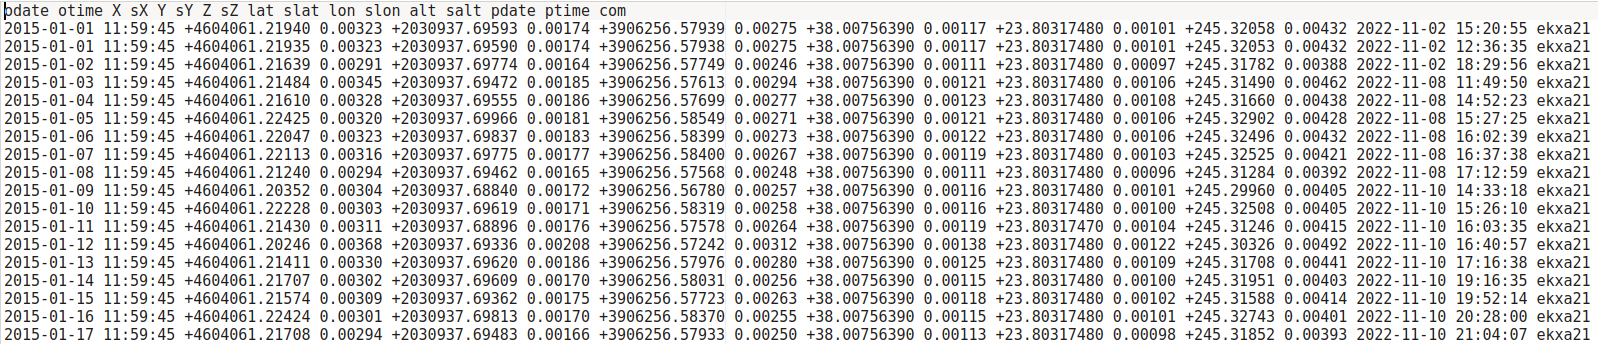
\includegraphics[width=.97\textwidth]{cts_screen.png}
  \end{center}
\end{frame}
\note{}

 % ------------------------------------------------------------------------------
\begin{frame}
  \frametitle{Ανάλυση χρονοσειρών θέσης}
  \framesubtitle{Πρόγραμμα - παράμετροι}
  \label{}
  \begin{columns}[T]
    \begin{column}{.5\textwidth}
      Ανάλυση χρονοσειρών θέσης με το λογισμικό πακέτο Hector \citep{Bos2012}
      \begin{itemize}\setlength\itemsep{1em}
        \item Τεκτονικές ταχύητες (γραμμικό μοντέλο)
        \item offsets/jumps: κυρίως λόγο επίδρασης σεισμών καθώς δεν υπάρχουν αλλαγές στον εξοπλισμό.
        \item Αρμονικά σήματα
        \item Αλλαγές ταχυτήτων (πχ. Σαντορίνη)
        \item Μετα-σεισμική παραμόρφωση
      \end{itemize}
    \end{column}
    \begin{column}{.5\textwidth}
      \begin{center}
      \vskip-.5cm
        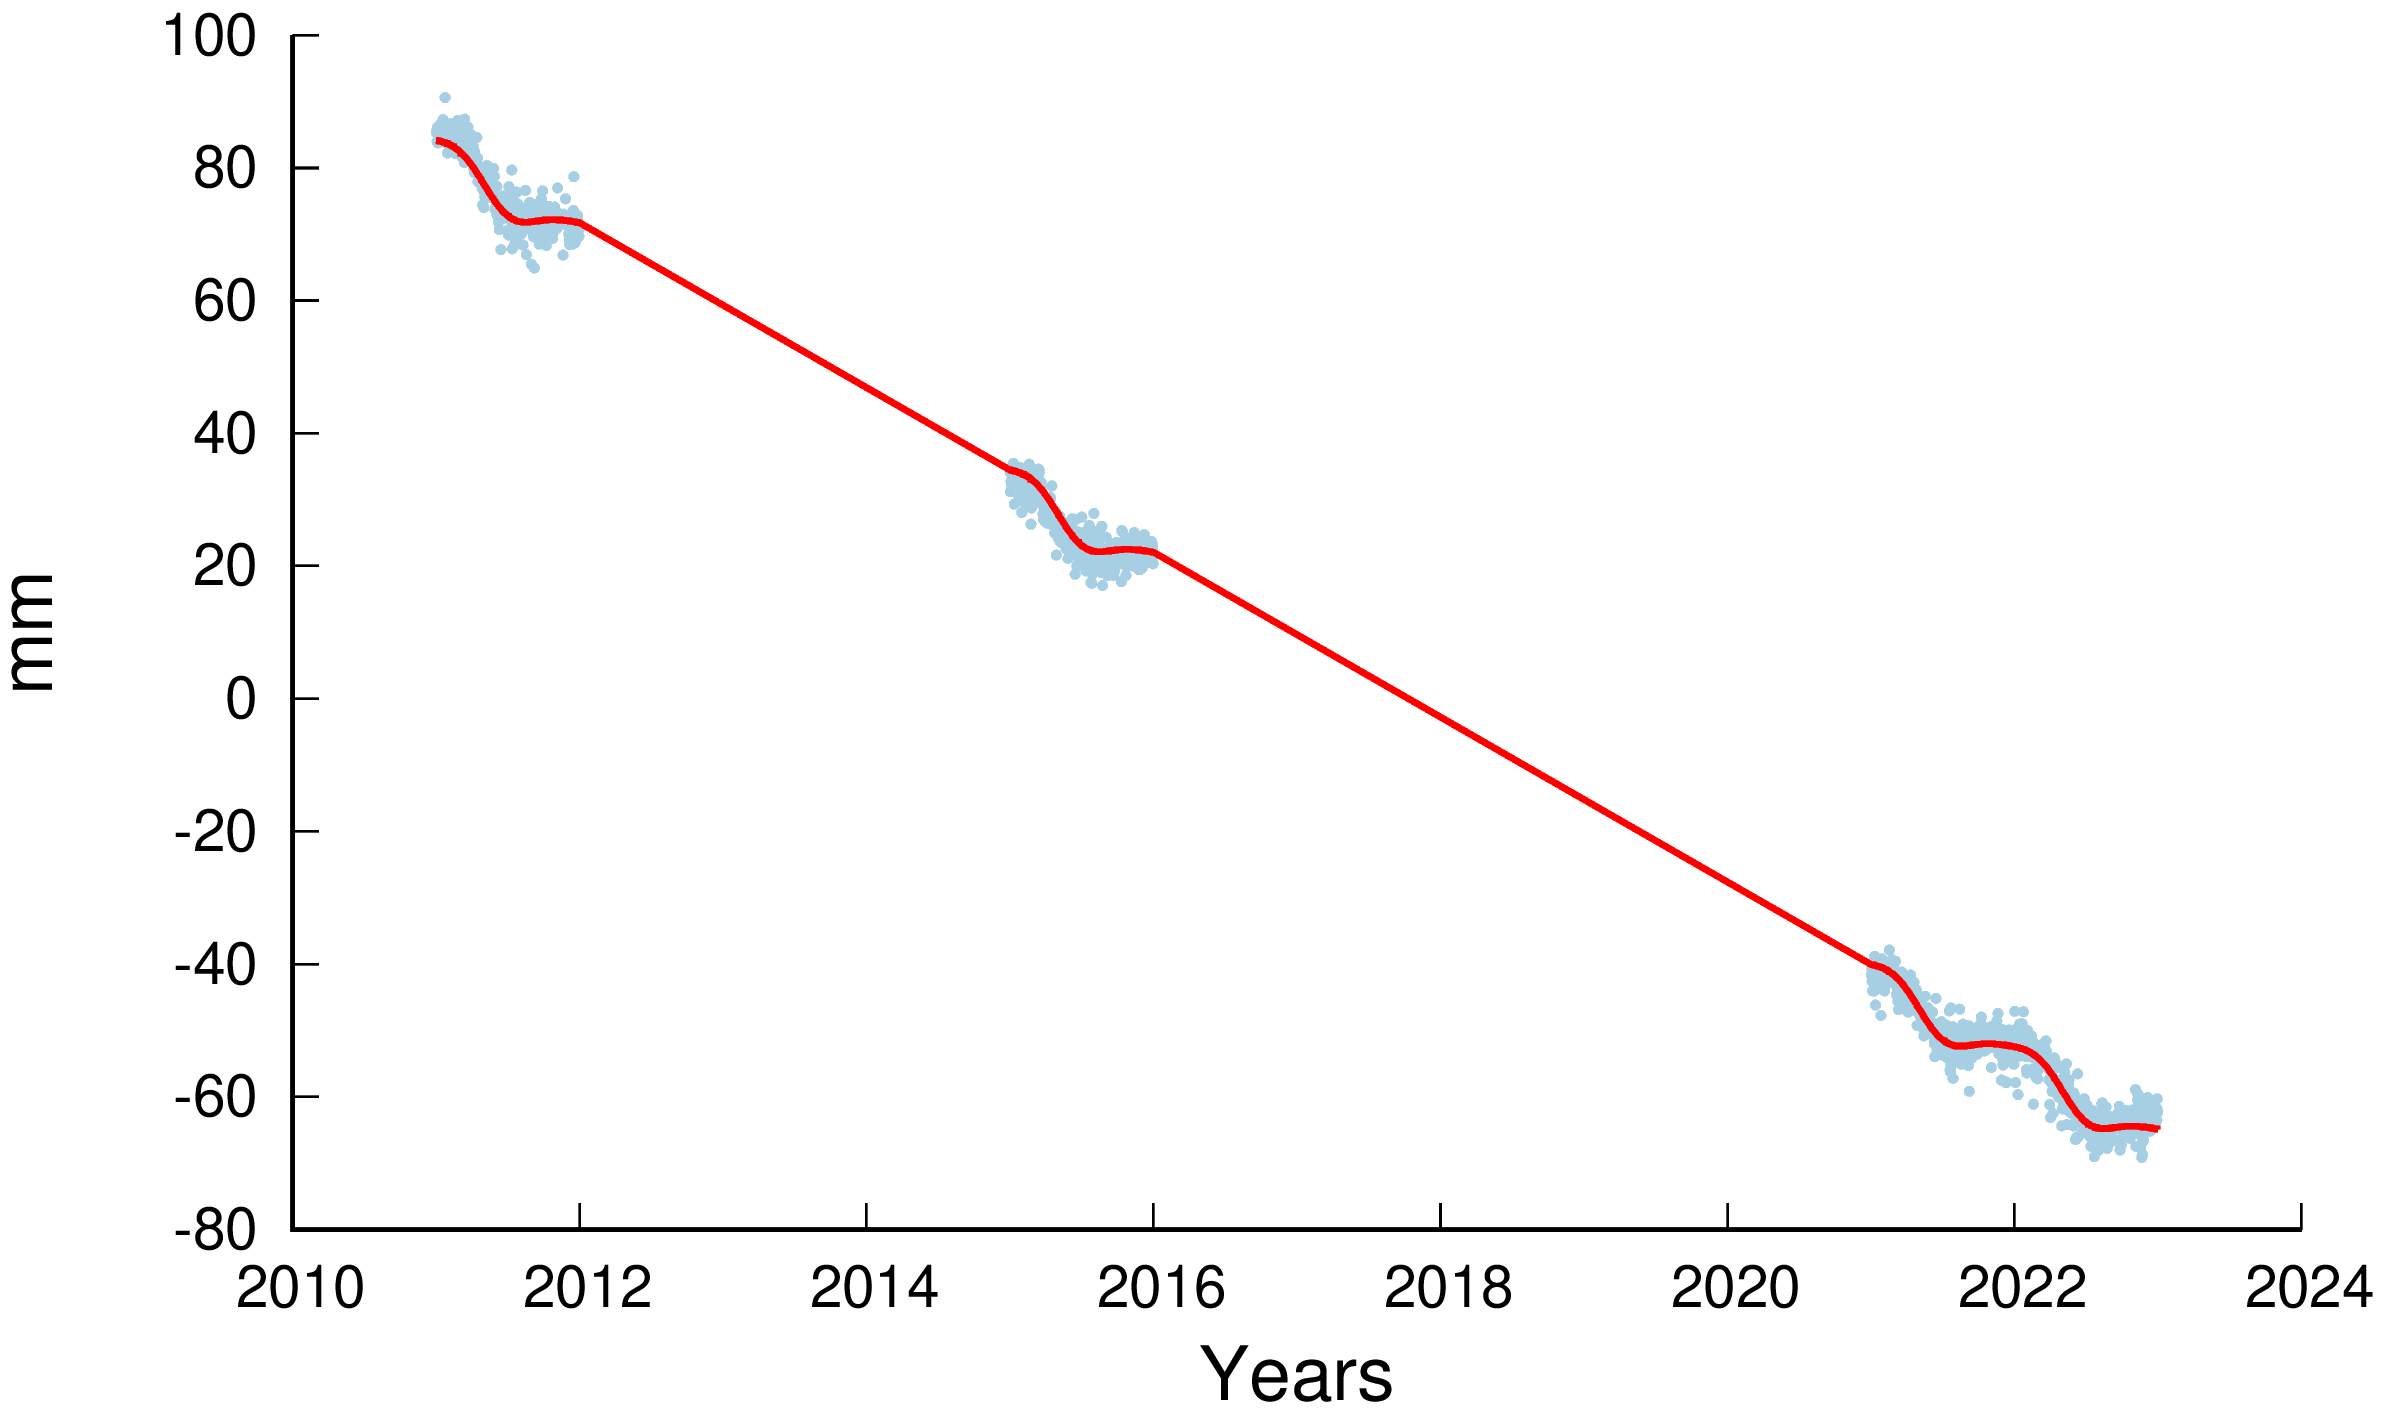
\includegraphics[width=.7\textwidth]{002a_0_data.png}
      \end{center}
      \begin{center}
        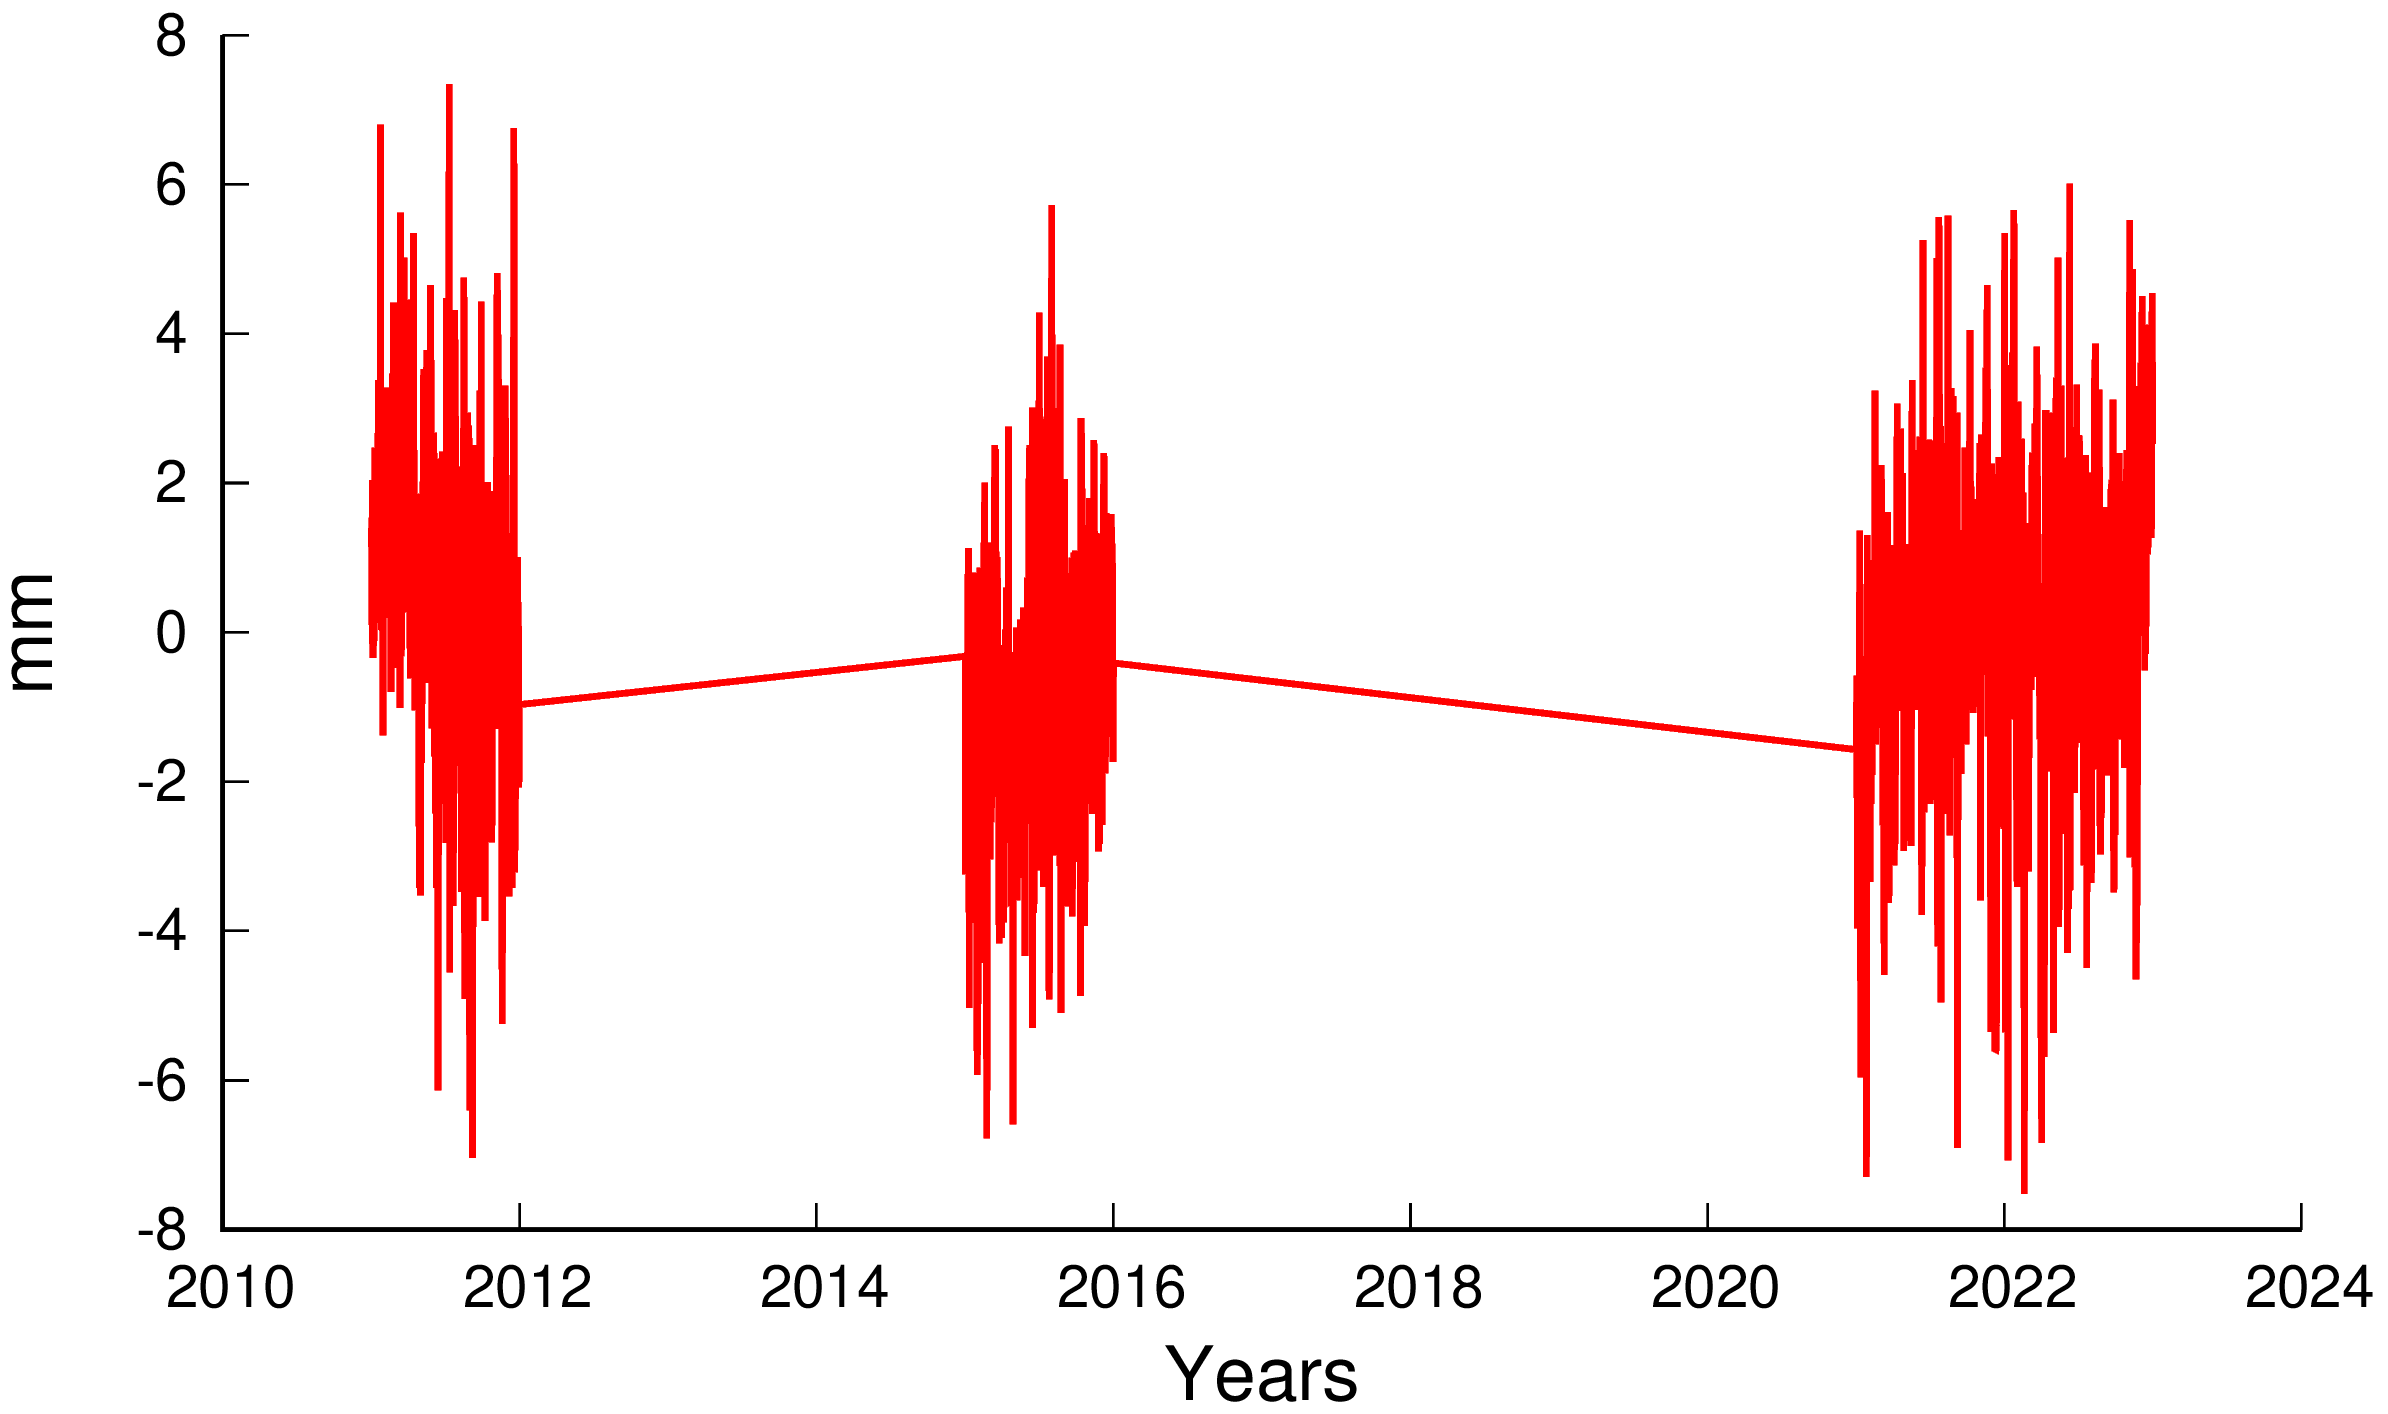
\includegraphics[width=.7\textwidth]{002a_0_res.png}
      \end{center}
    \end{column}
  \end{columns}
\end{frame}
\note{}


 % ------------------------------------------------------------------------------
\begin{frame}
  \frametitle{Απομάκρυνση χονδροειδών σφαλμάτων - outliers}
  \framesubtitle{}
  \label{}
  
\end{frame}
\note{}

 % ------------------------------------------------------------------------------
\begin{frame}
  \frametitle{Προσδιορισμός ασυνεχειών - offsets}
  \framesubtitle{}
  \label{}
  \vskip-1cm
  \begin{columns}[T]
    \begin{column}{.33\textwidth}
      \begin{center}
      Station:\textbf{040A}\\
         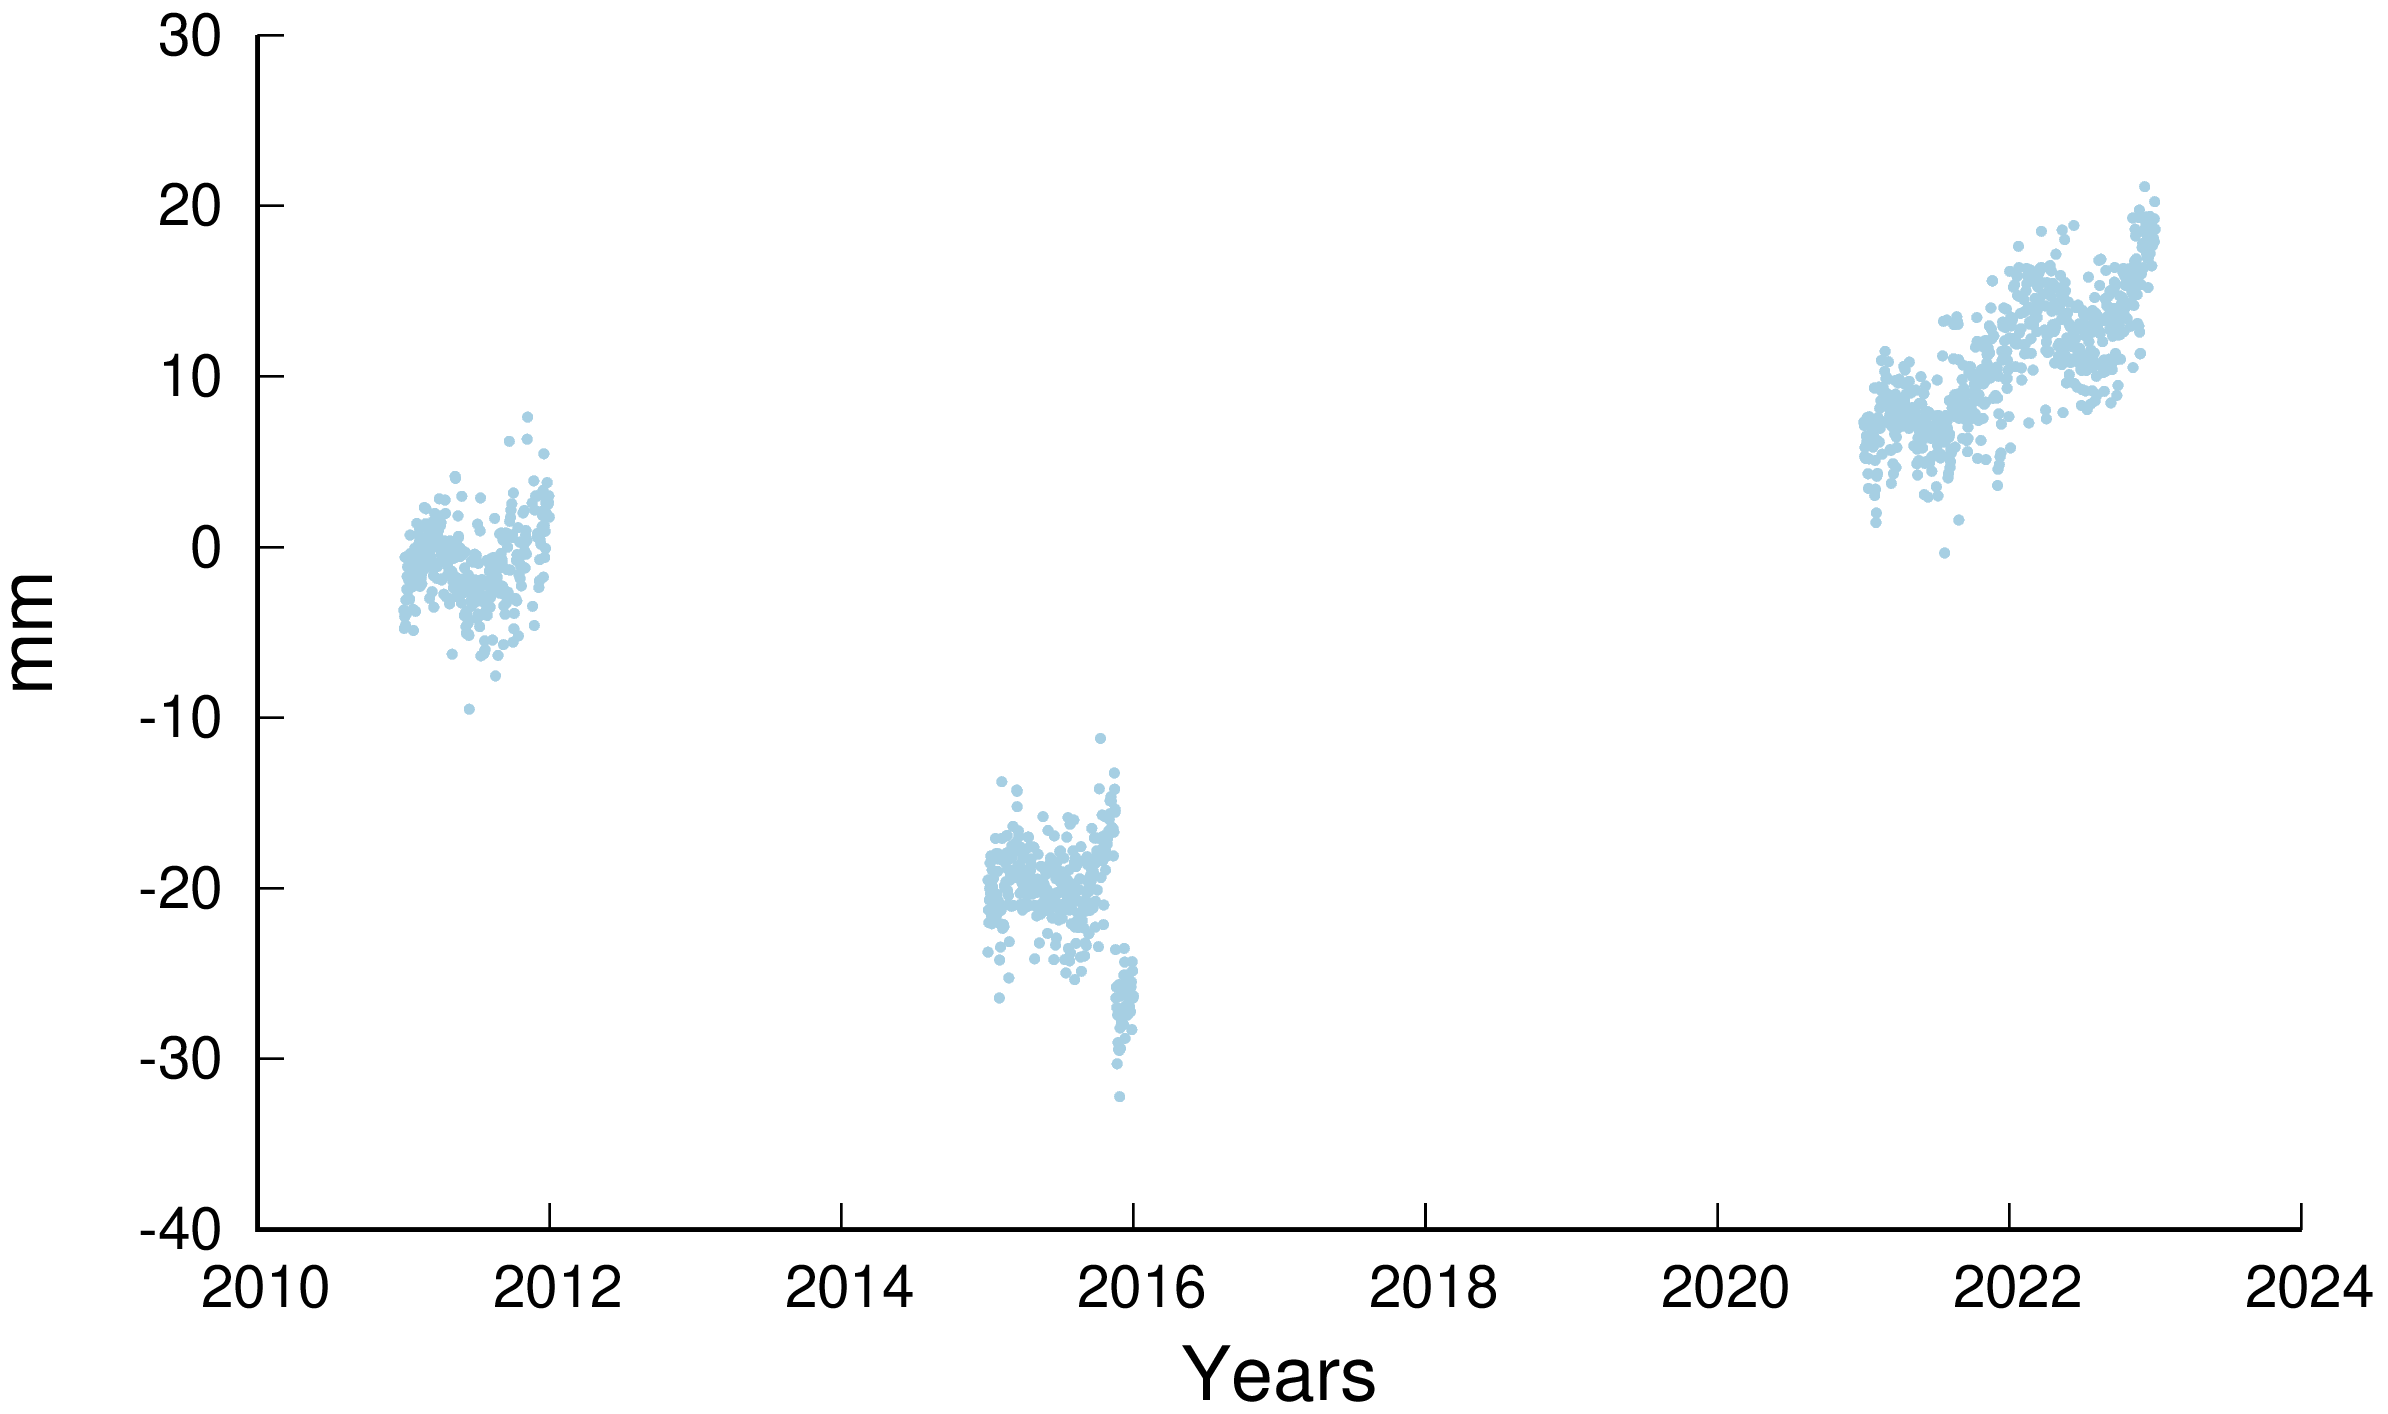
\includegraphics[width=.75\textwidth]{040a_0_data_nomodel.png}\\
         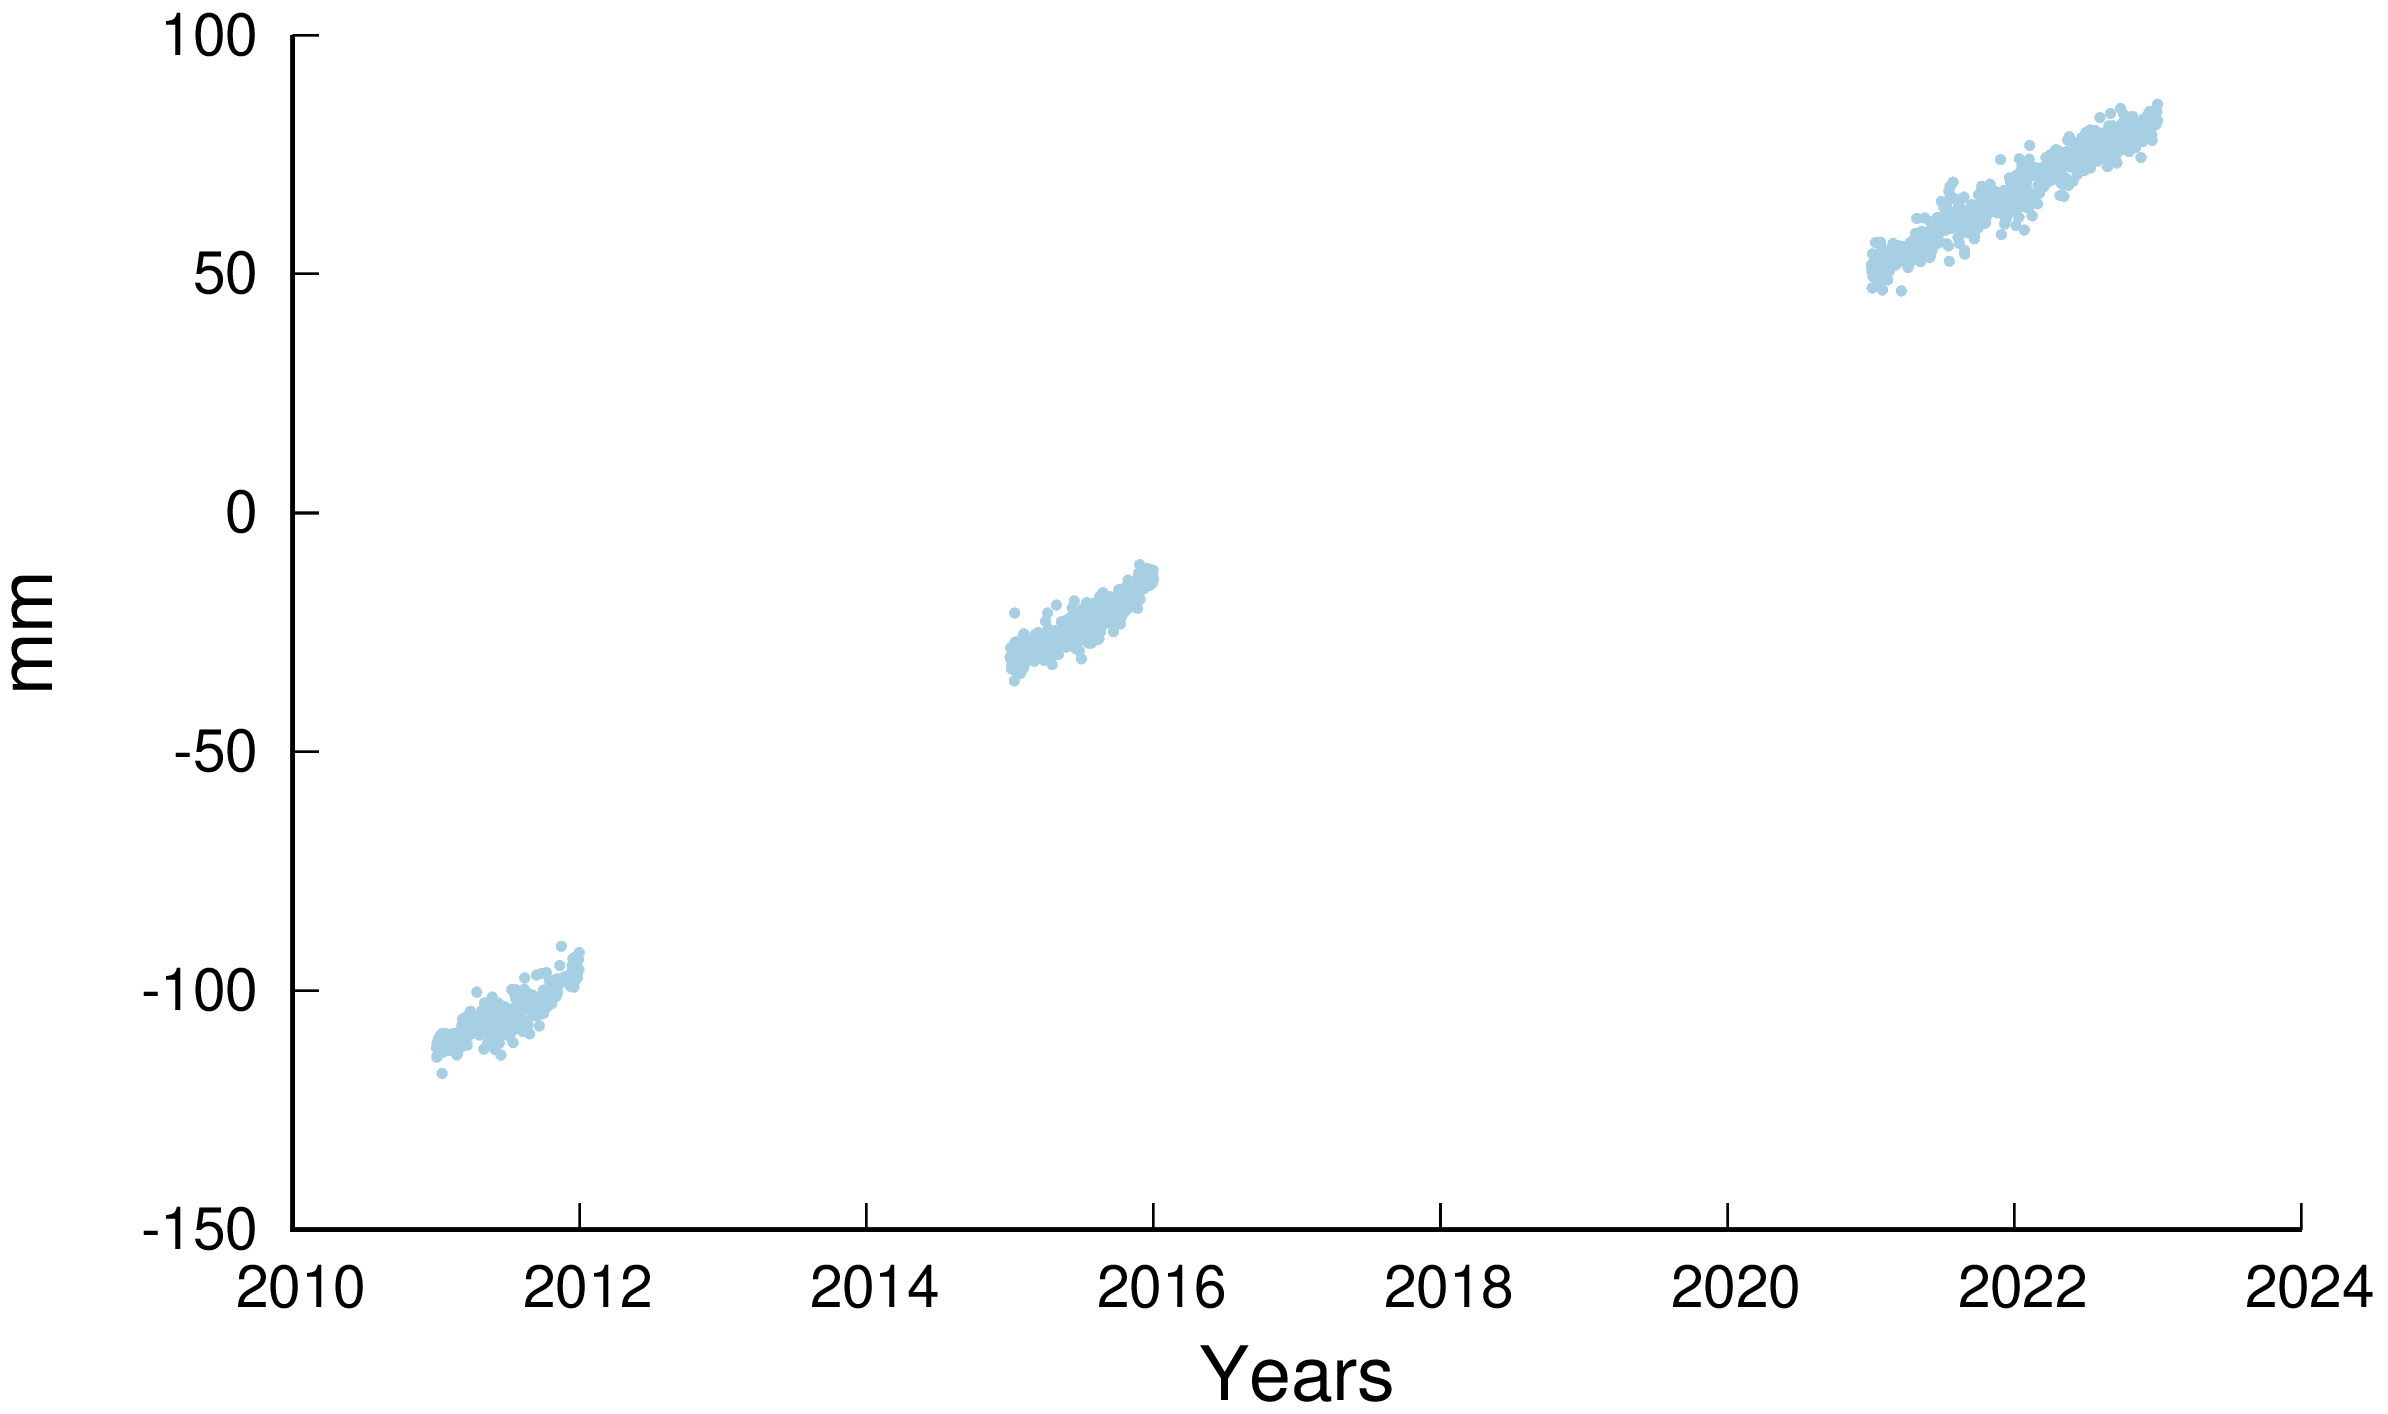
\includegraphics[width=.75\textwidth]{040a_1_data_nomodel.png}\\
         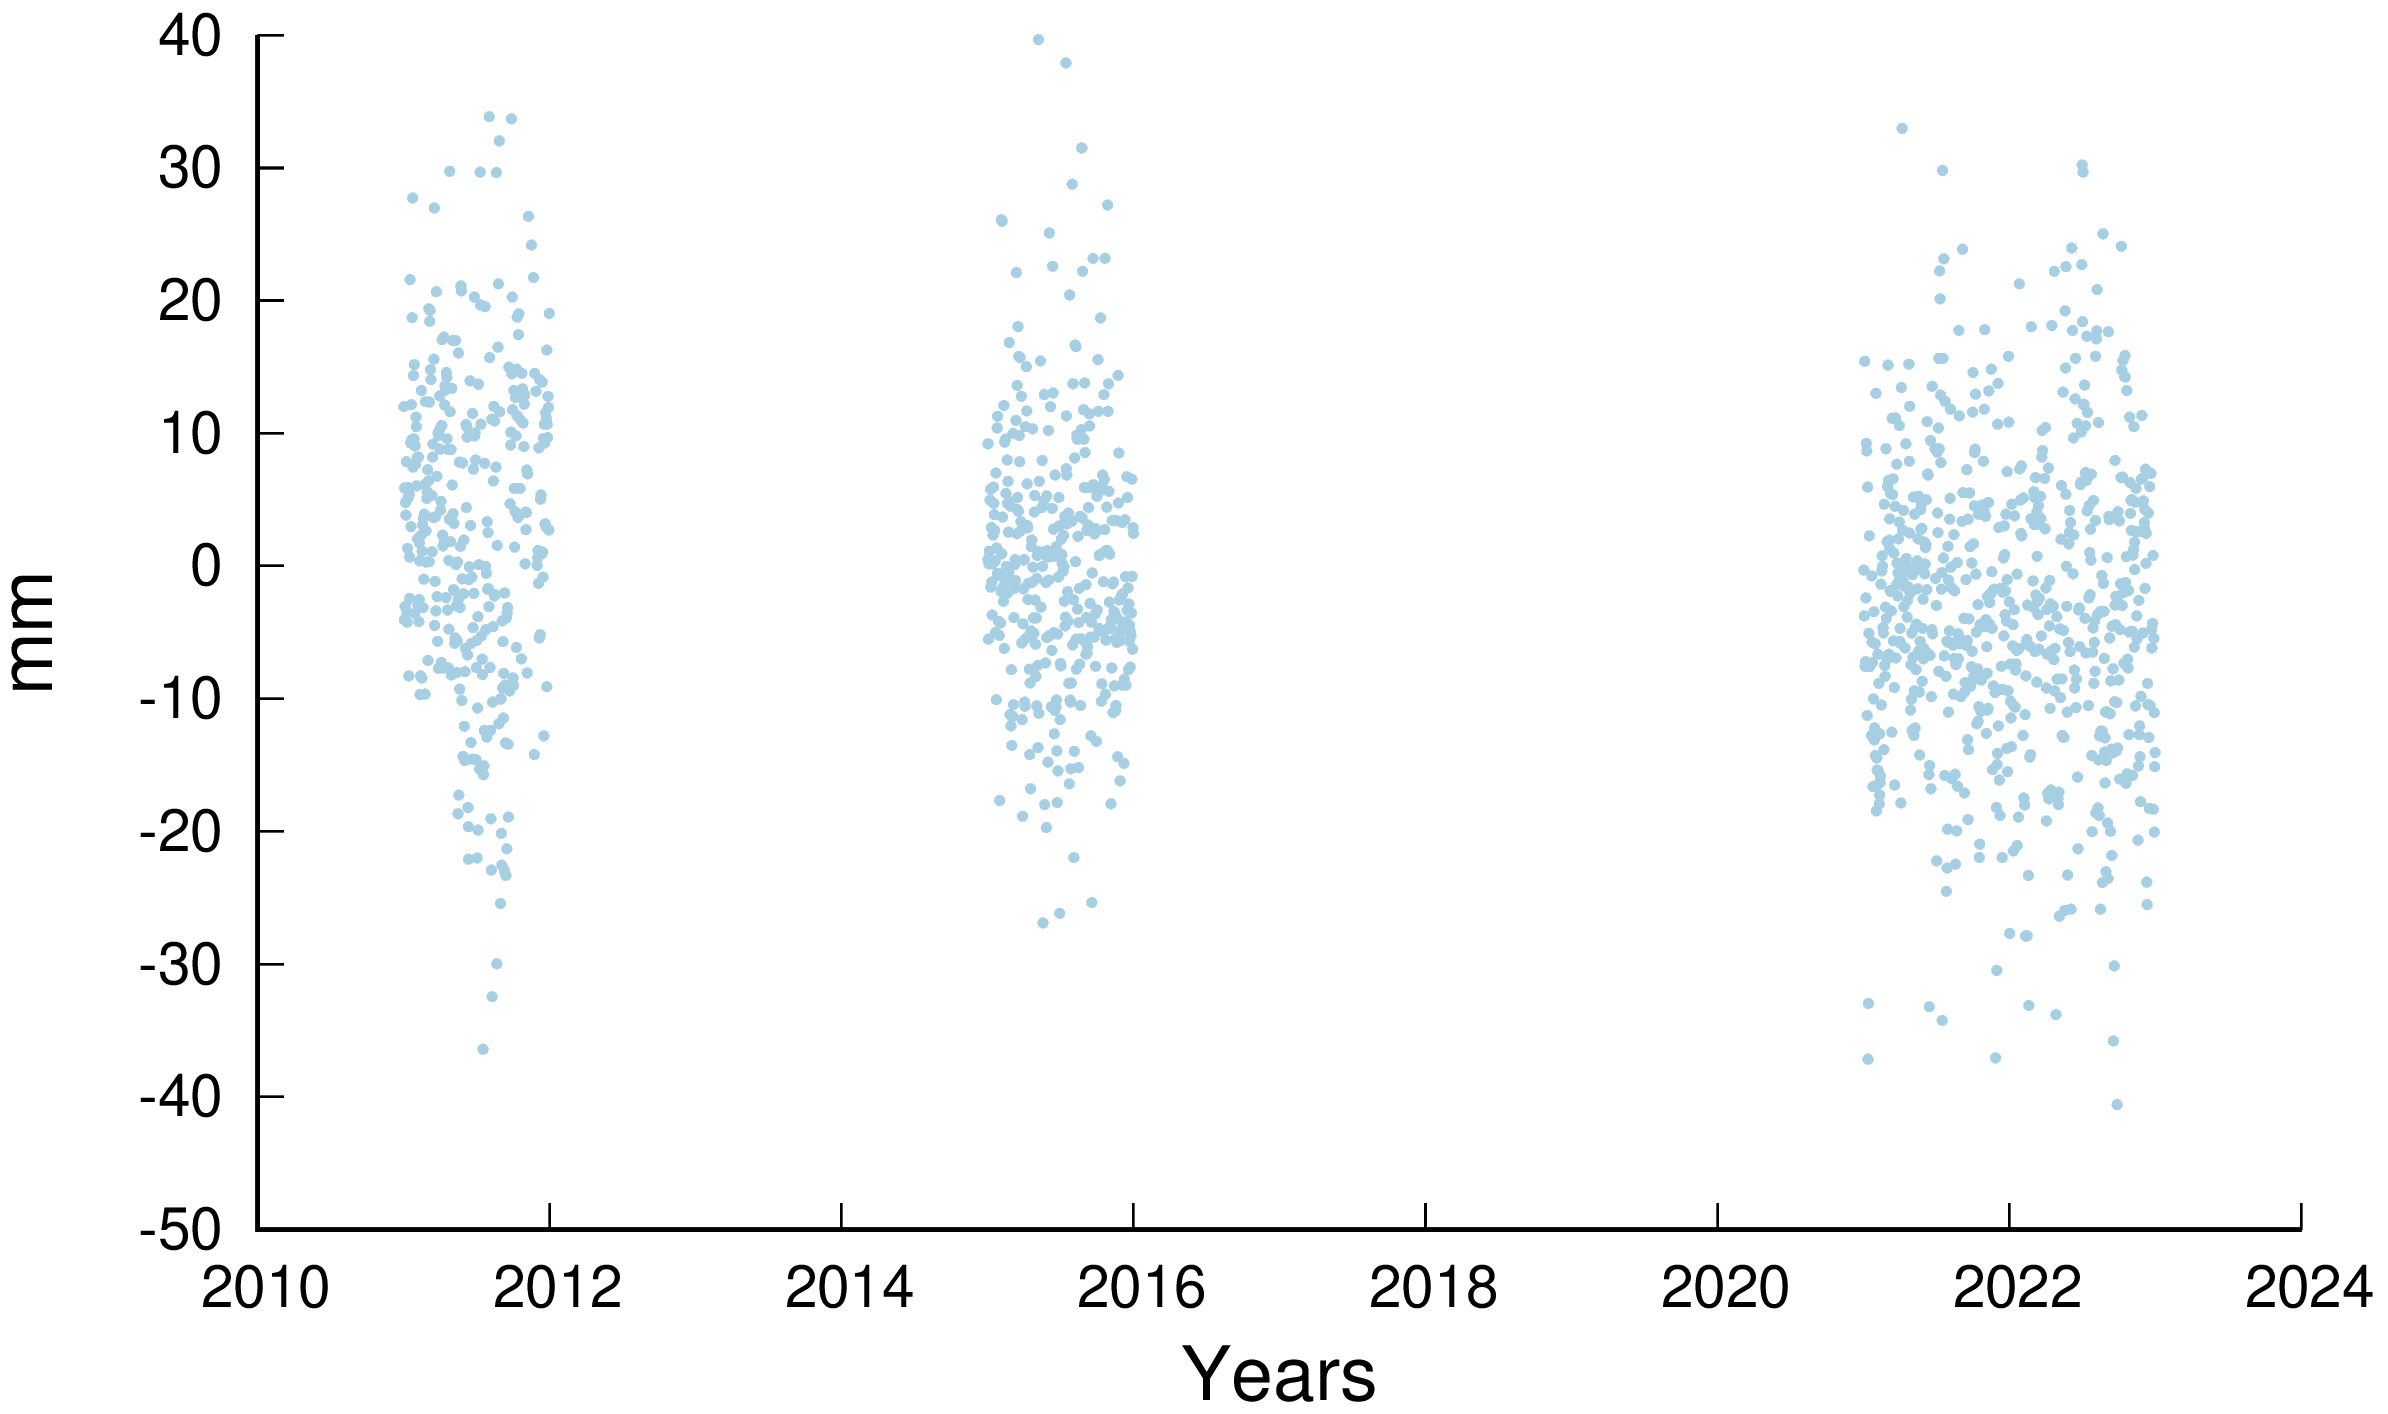
\includegraphics[width=.75\textwidth]{040a_2_data_nomodel.png}
       \end{center} 
    \end{column}
    \begin{column}{.33\textwidth}
      \begin{center}
      Station:\textbf{057A}\\
         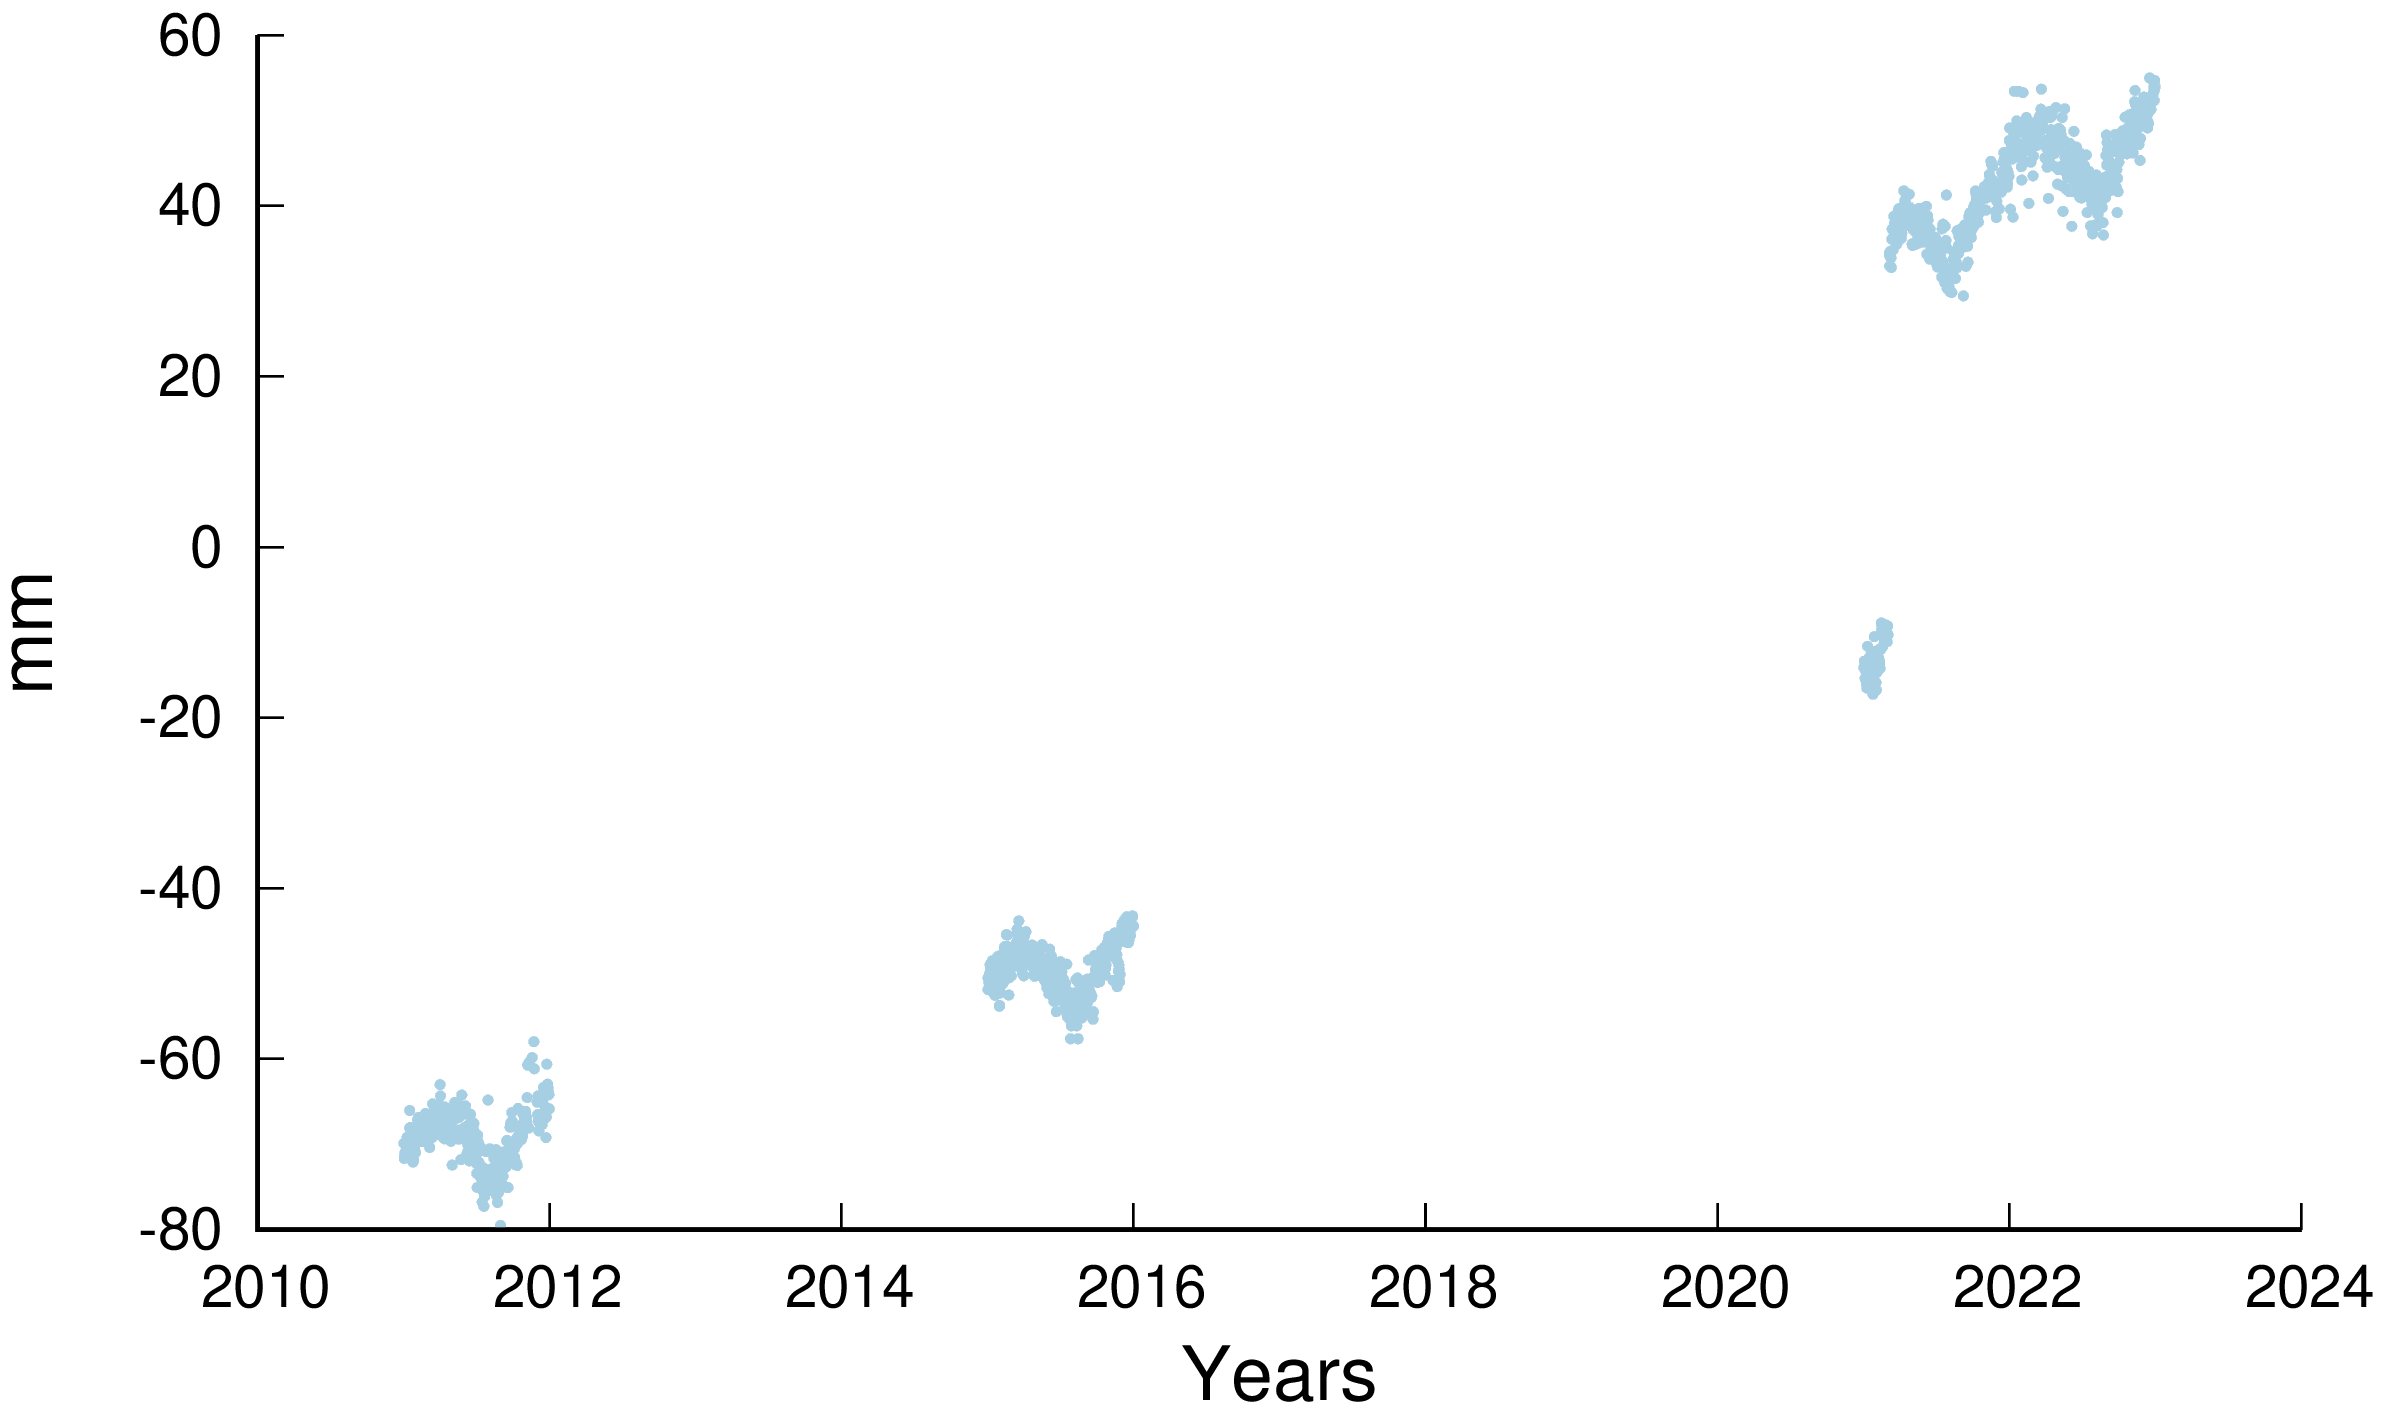
\includegraphics[width=.75\textwidth]{057a_0_data_nomodel.png}\\
         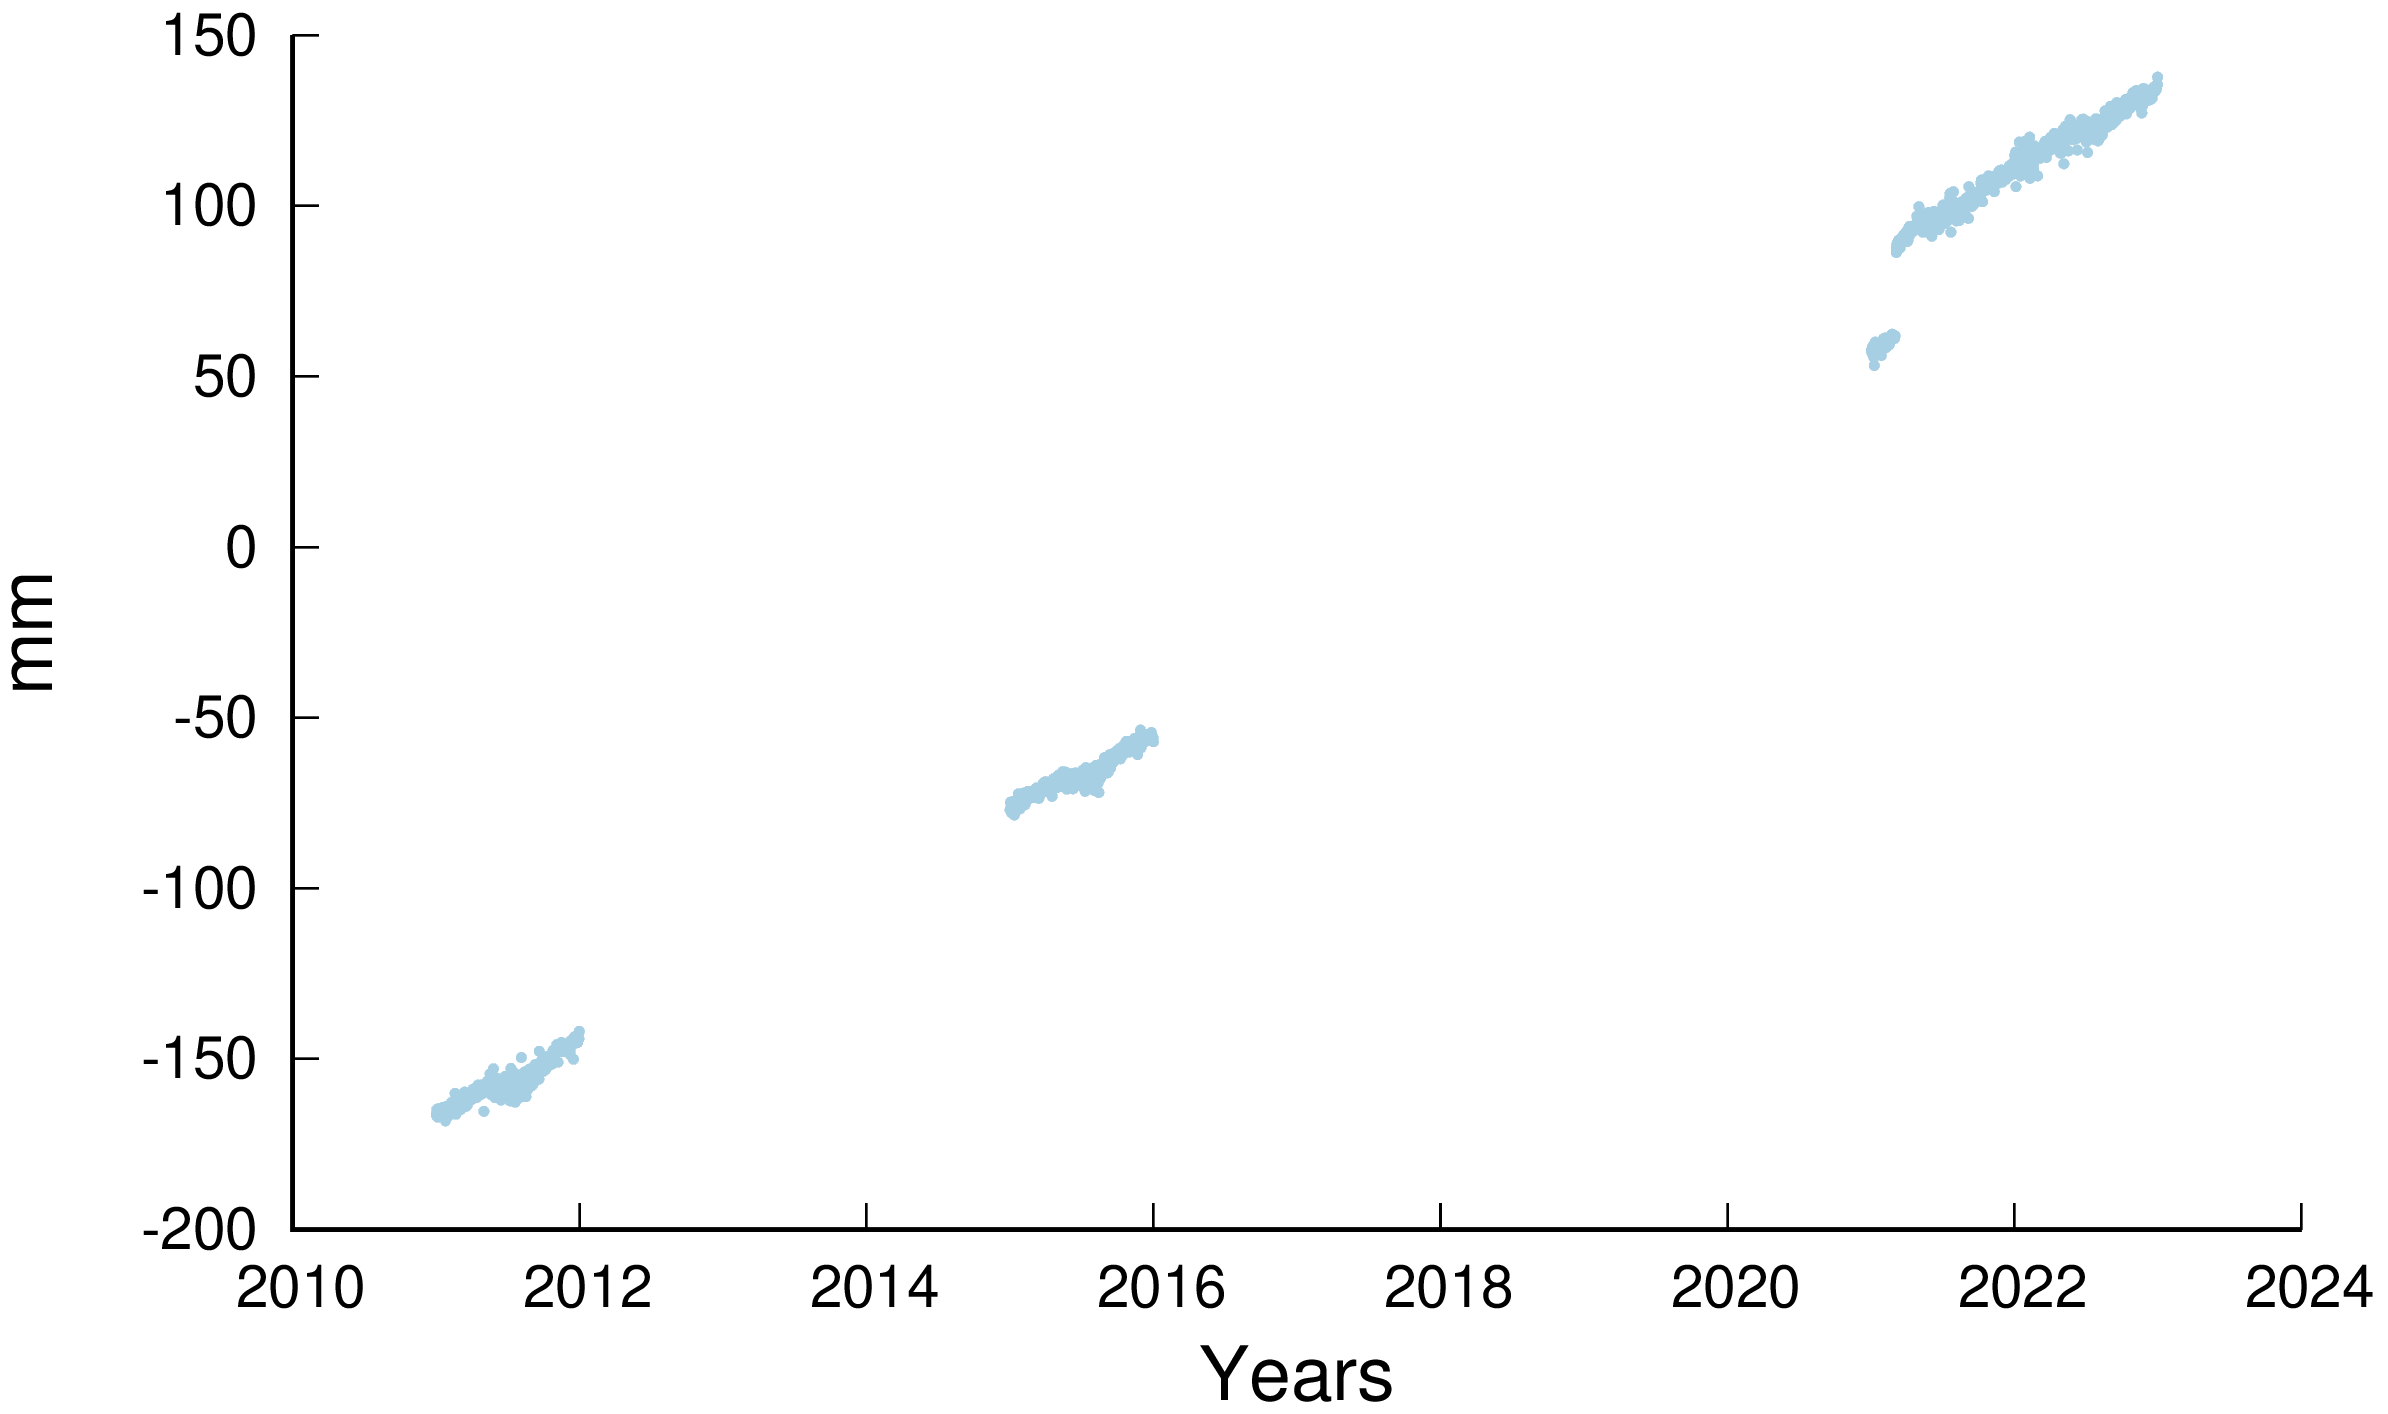
\includegraphics[width=.75\textwidth]{057a_1_data_nomodel.png}\\
         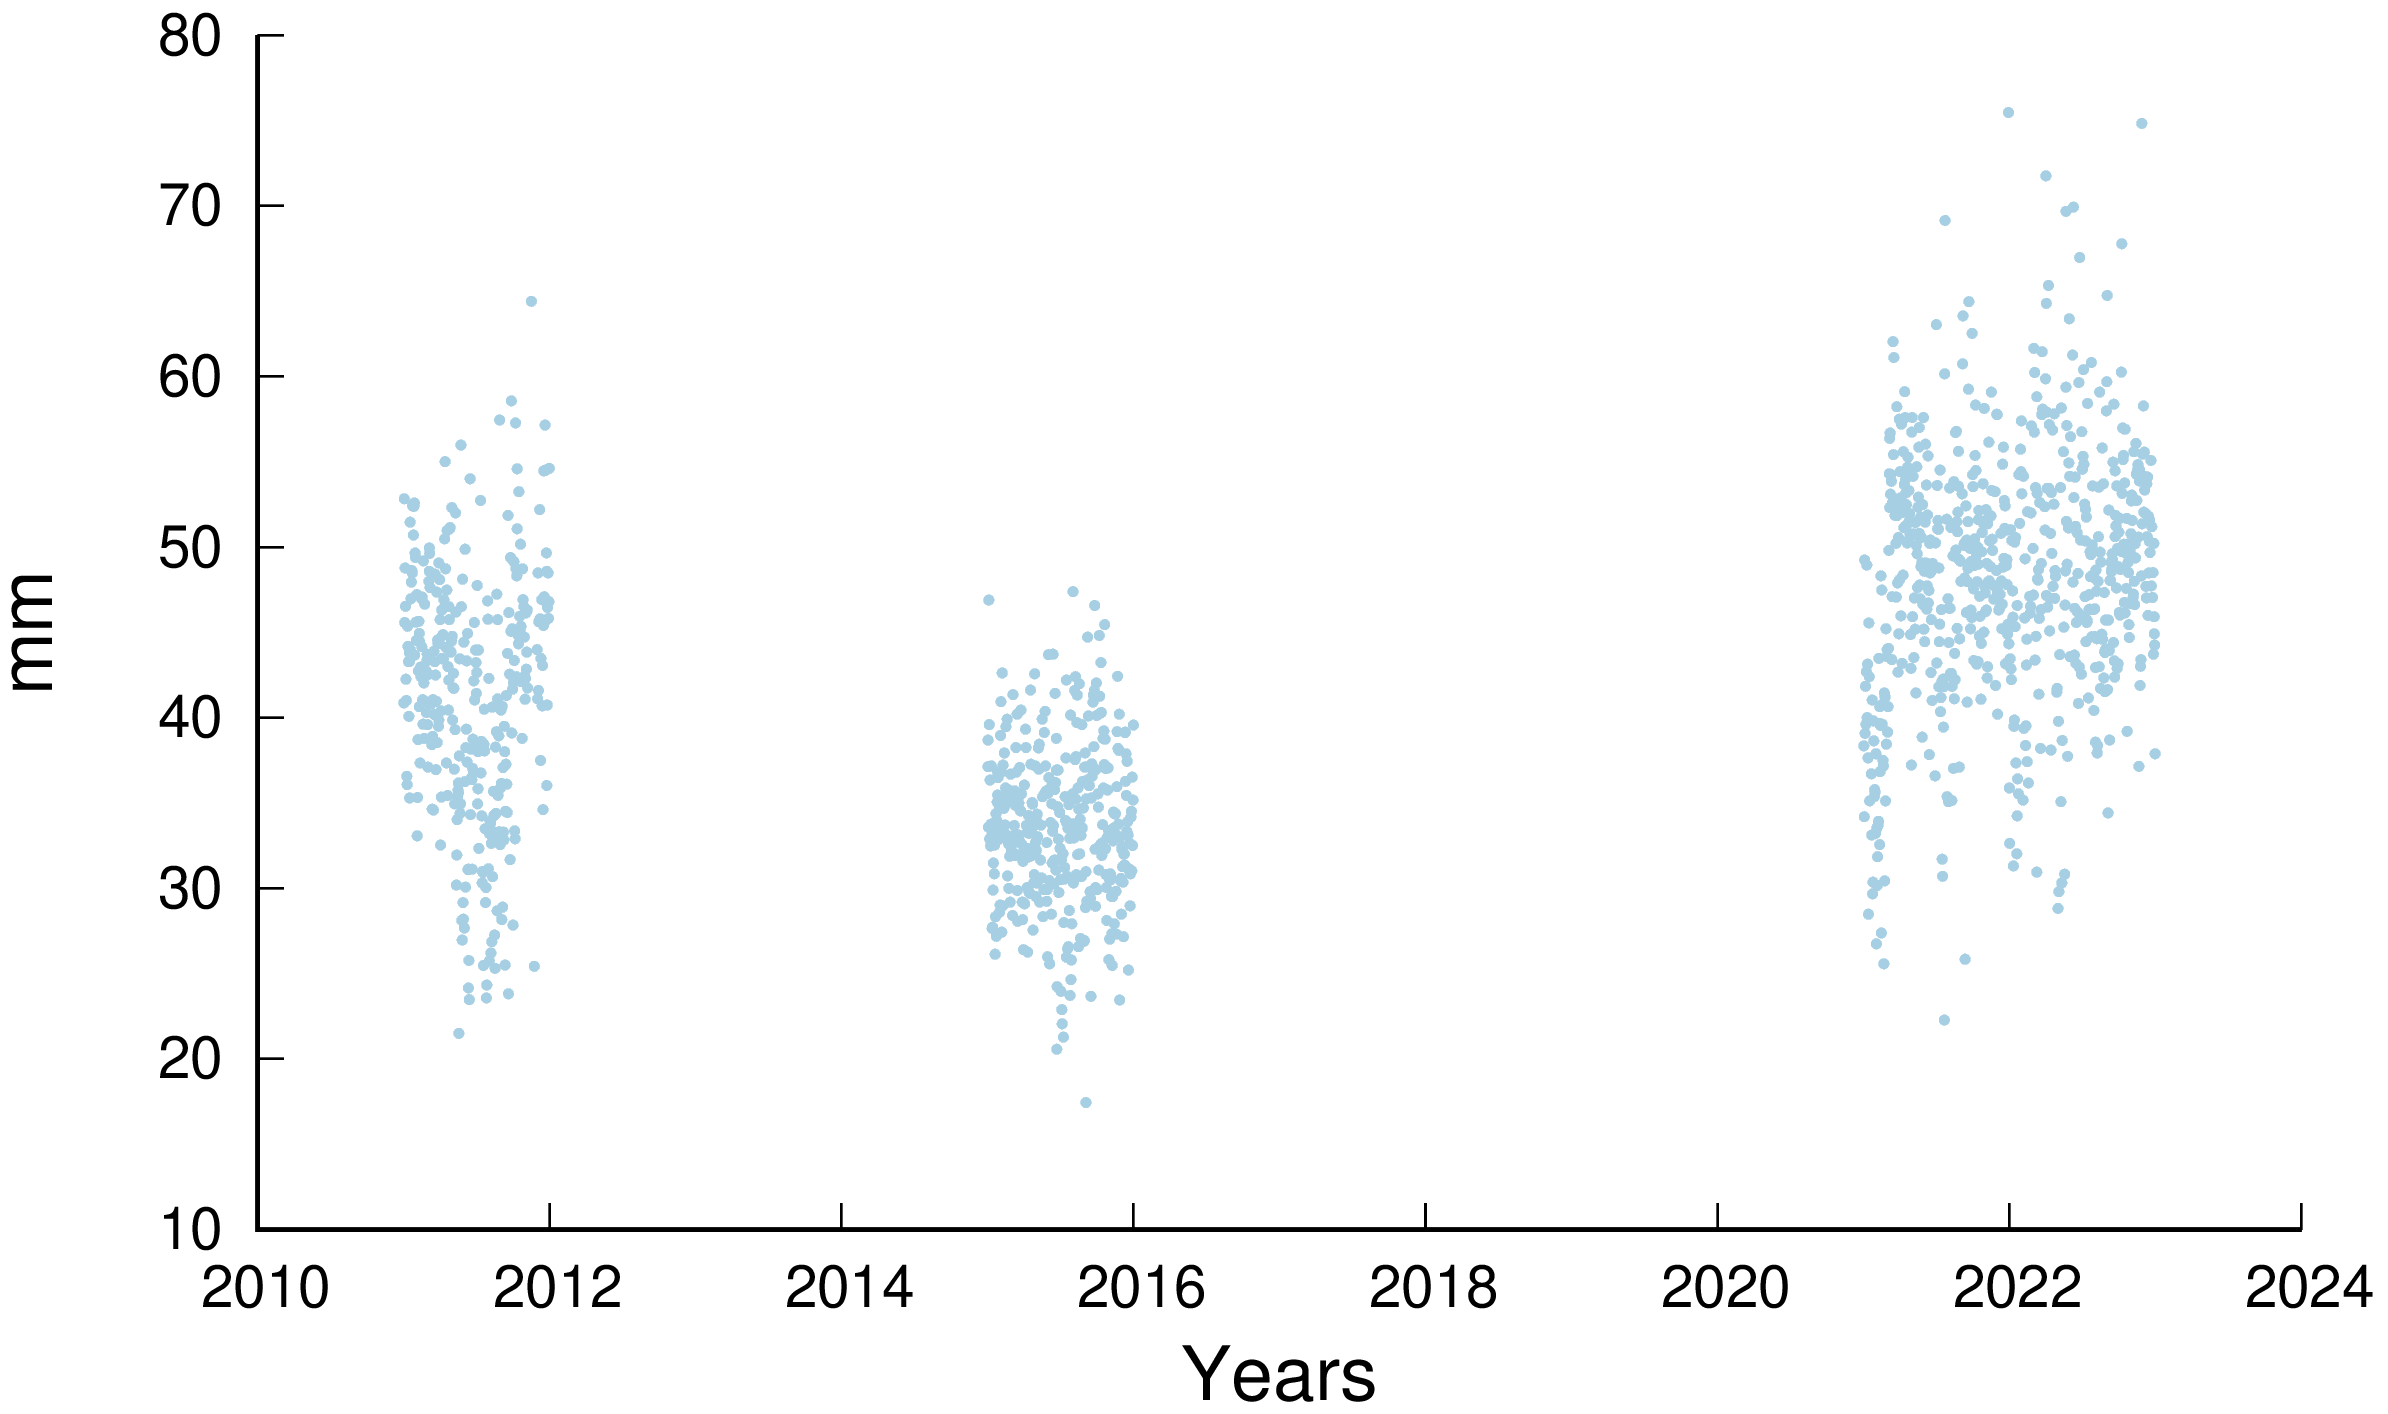
\includegraphics[width=.75\textwidth]{057a_2_data_nomodel.png}
       \end{center} 
    \end{column}
    \begin{column}{.33\textwidth}
      \begin{center}
      Station:\textbf{098A}\\
         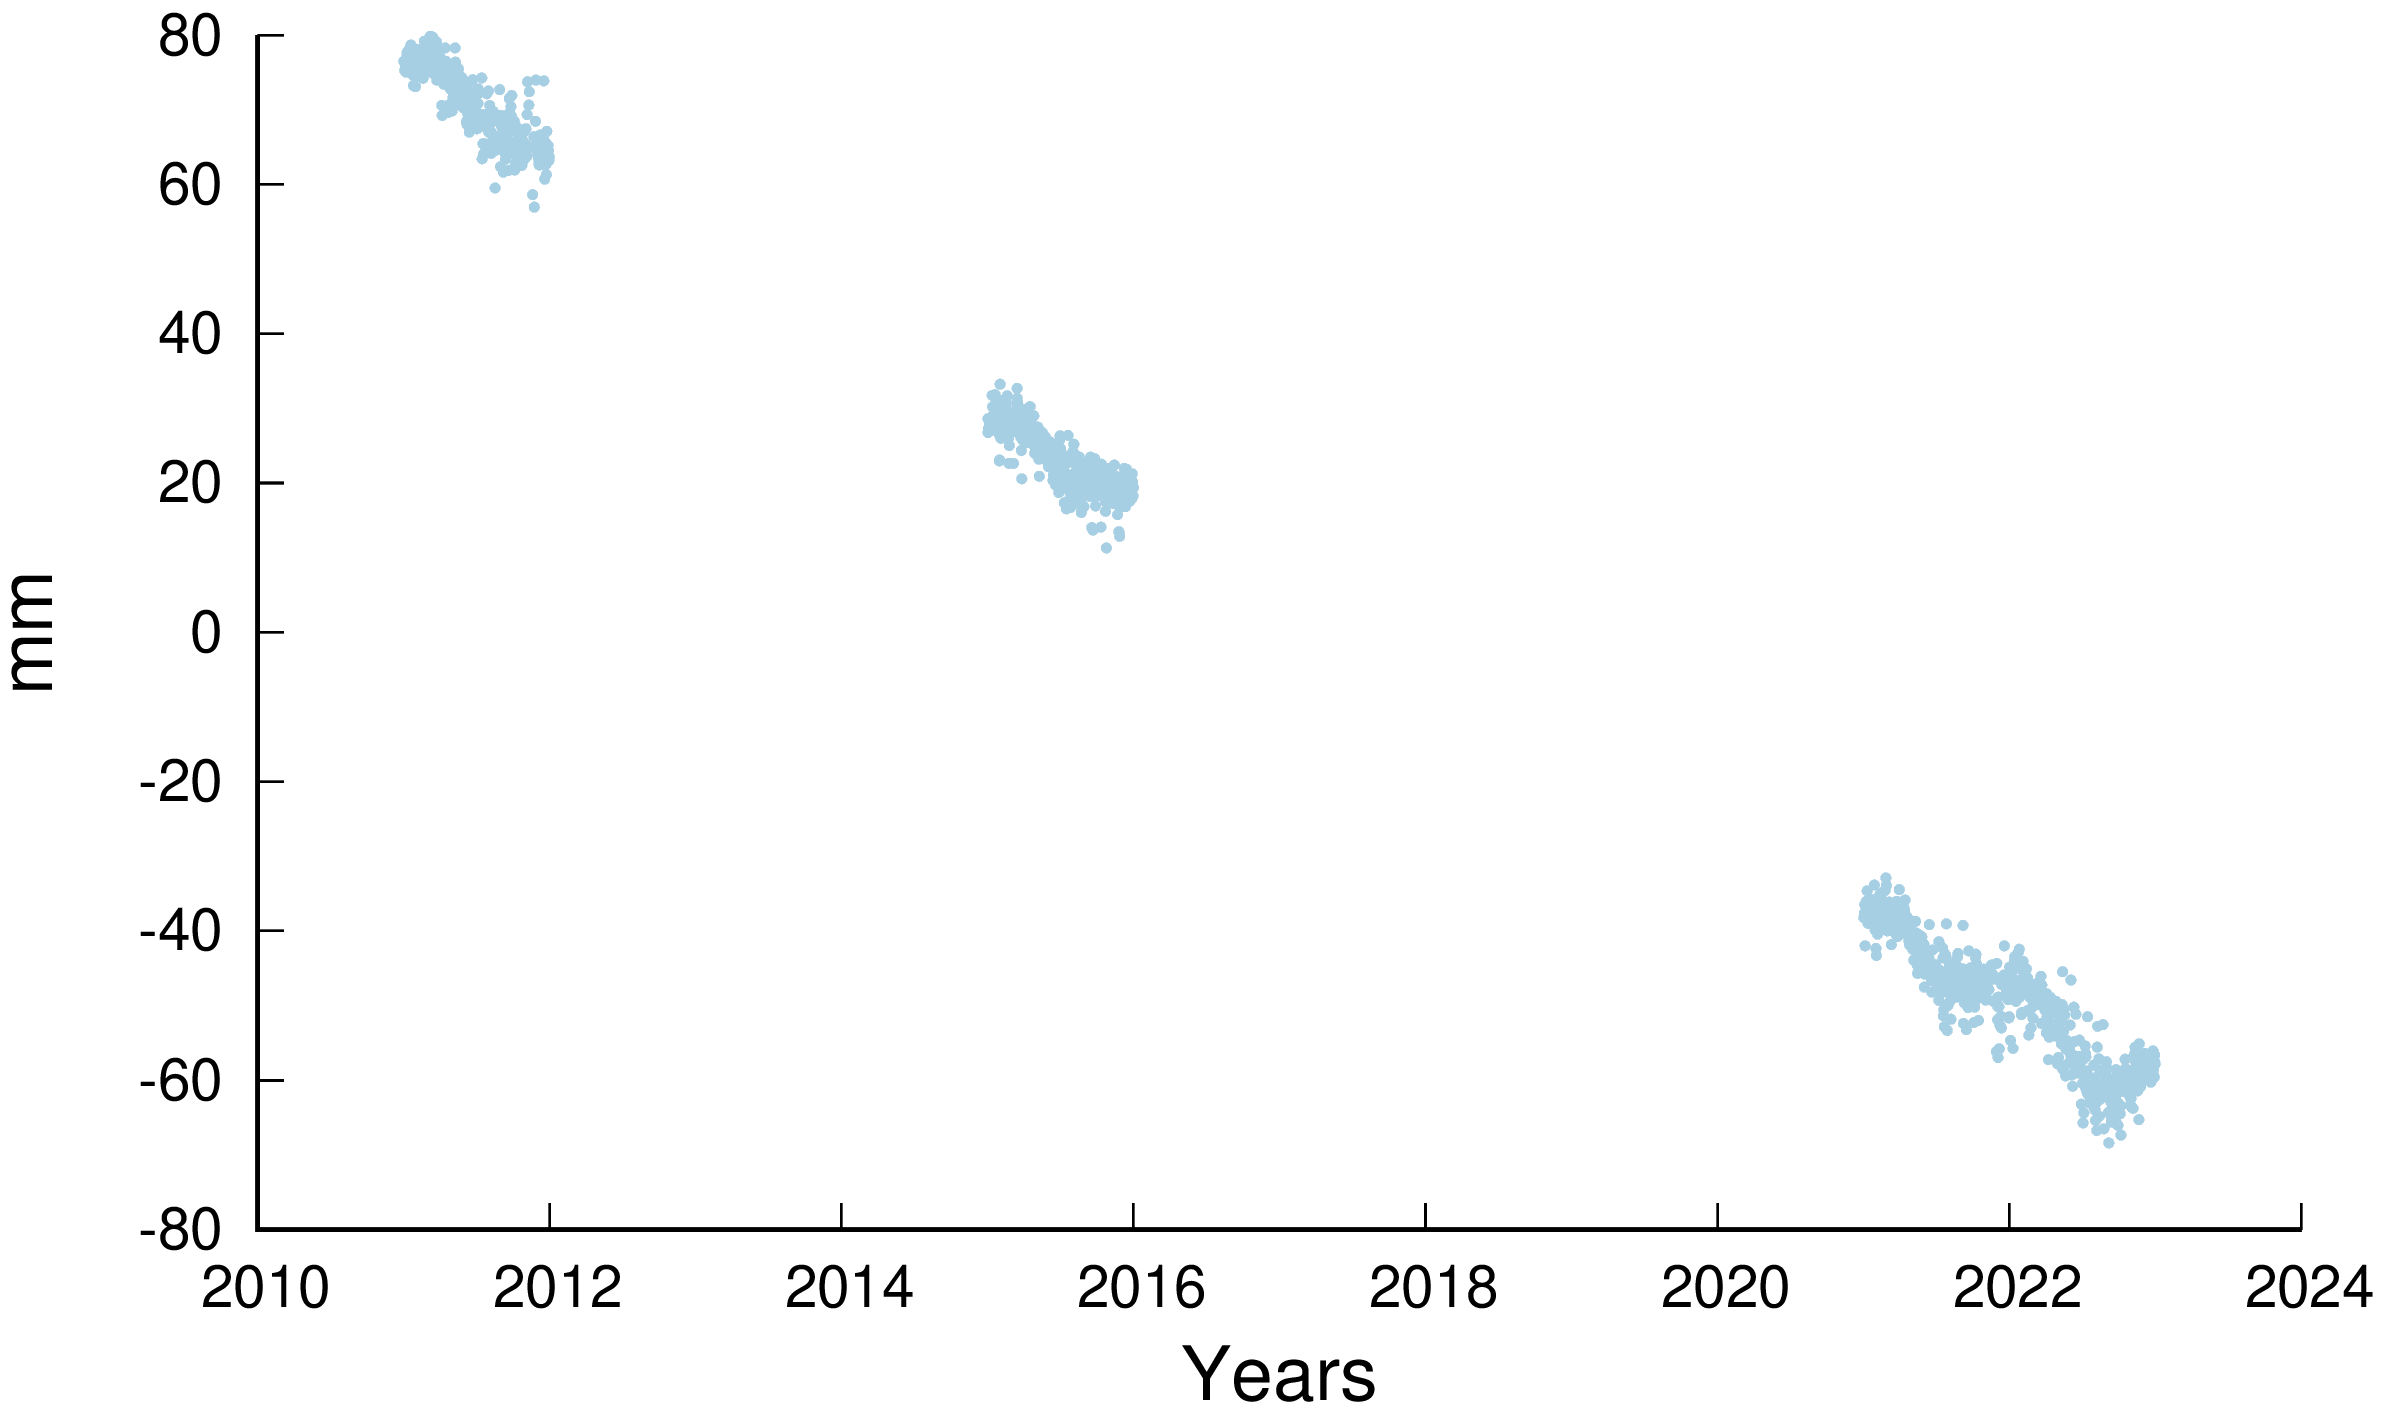
\includegraphics[width=.75\textwidth]{098a_0_data_nomodel.png}\\
         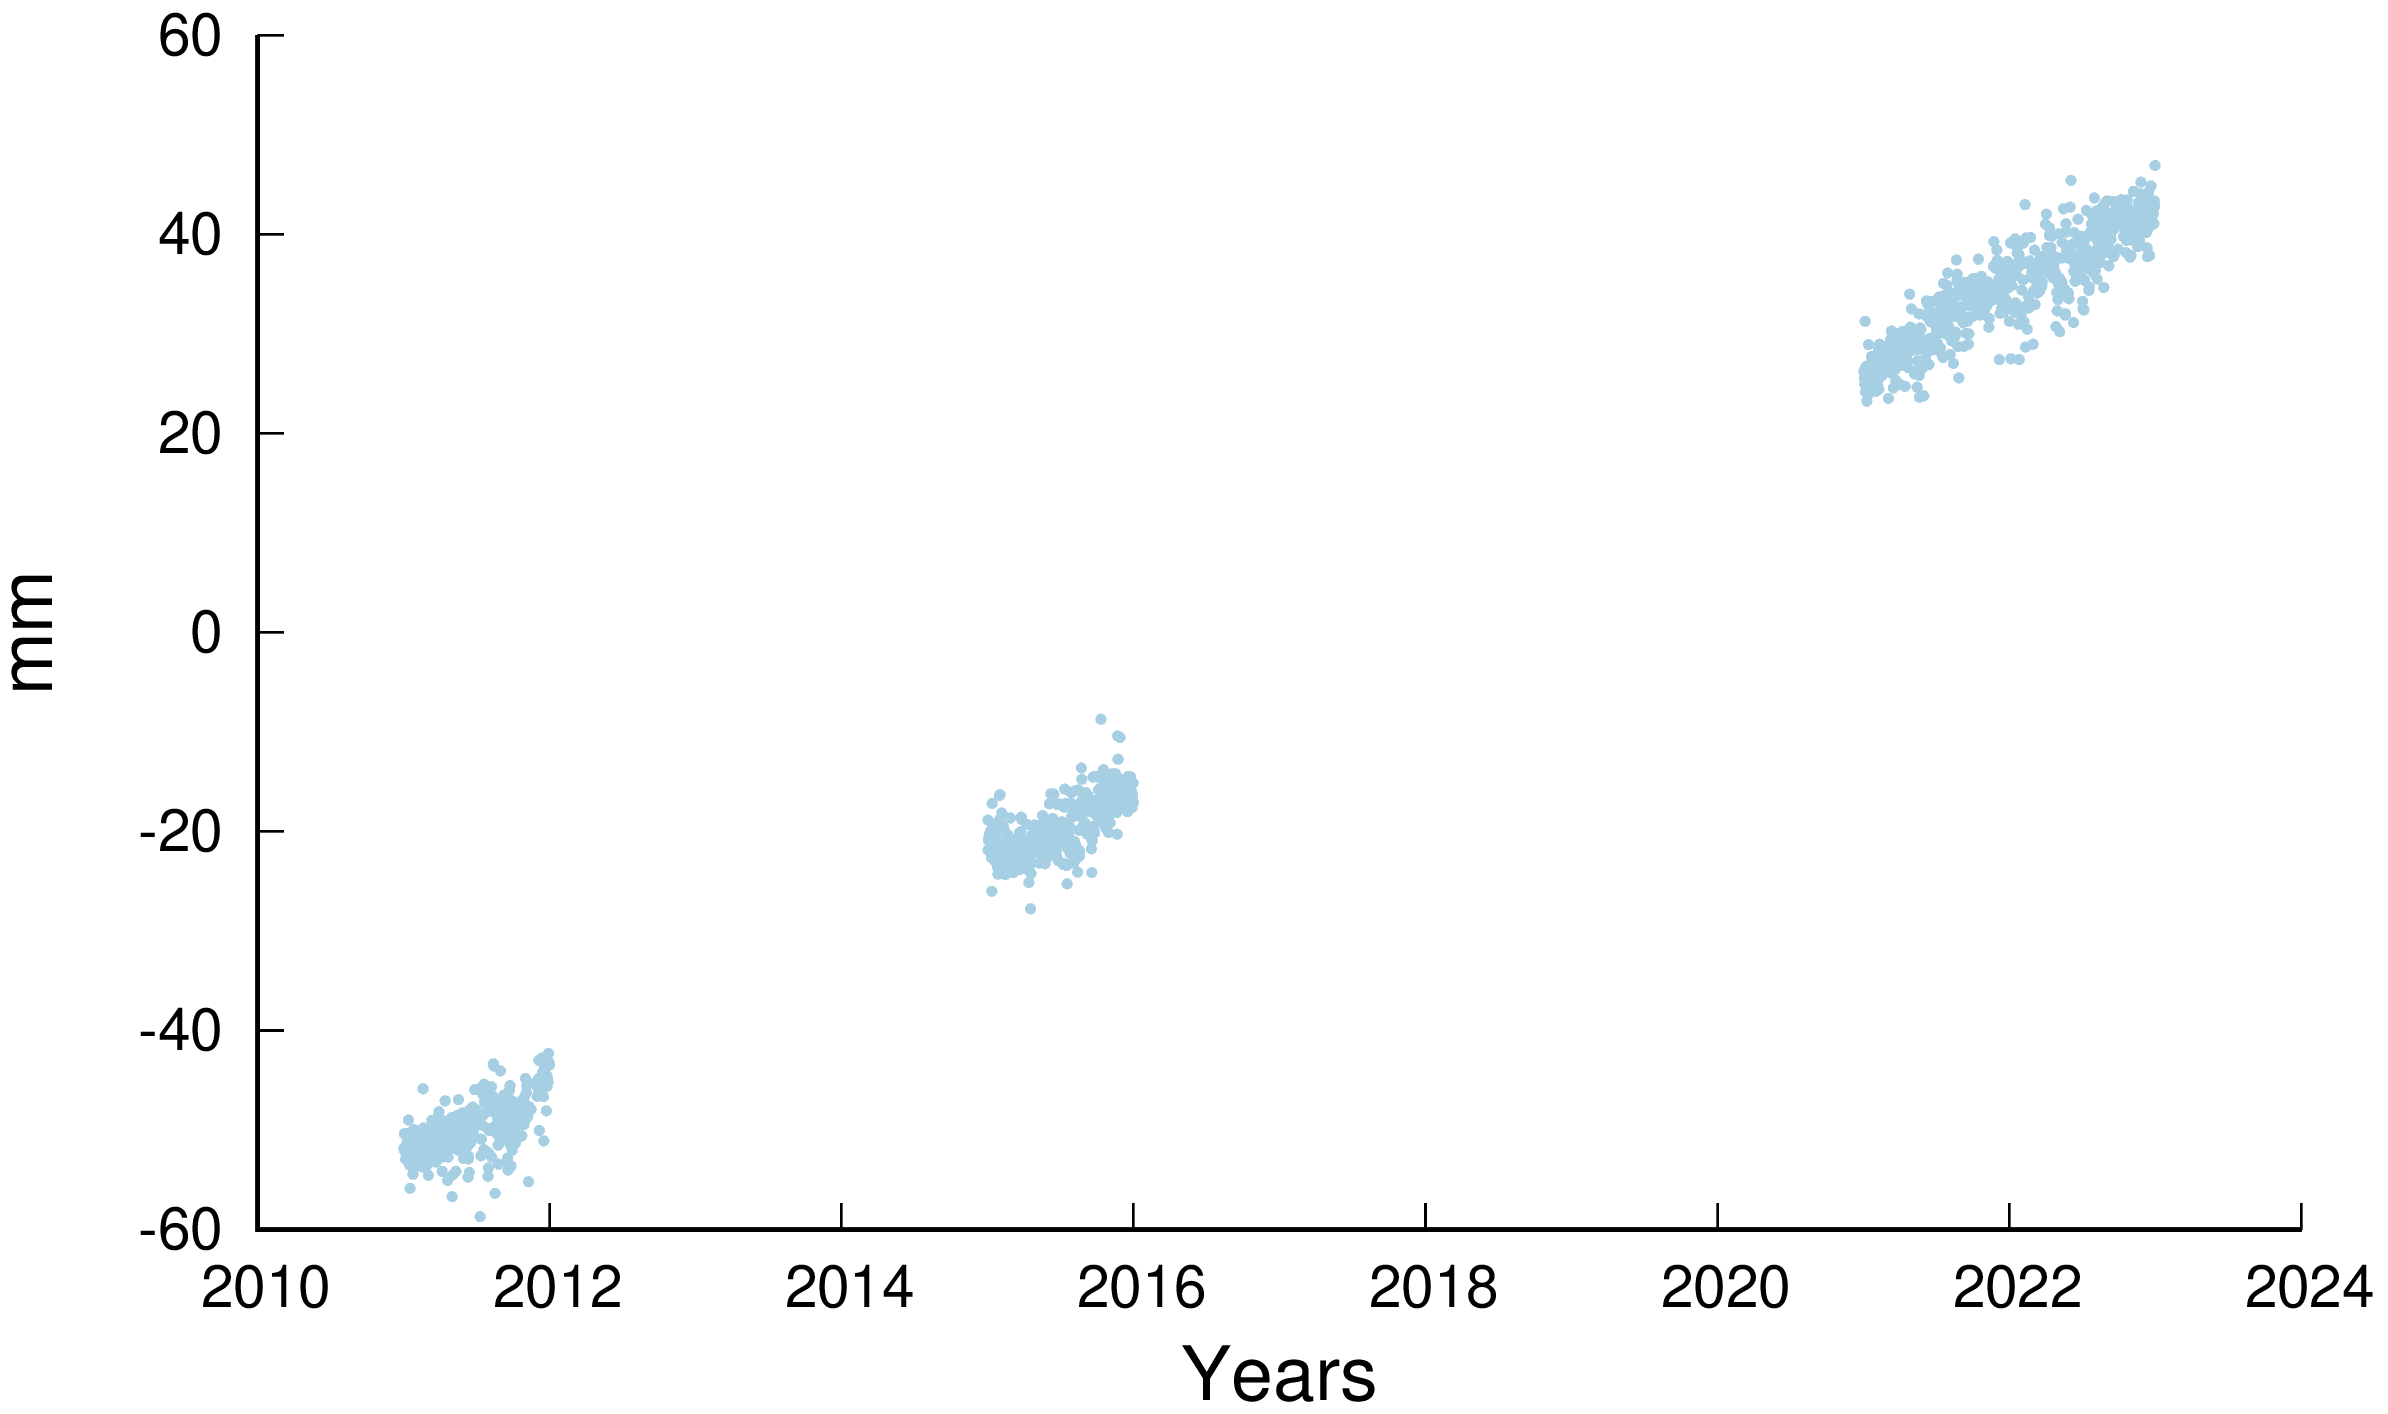
\includegraphics[width=.75\textwidth]{098a_1_data_nomodel.png}\\
         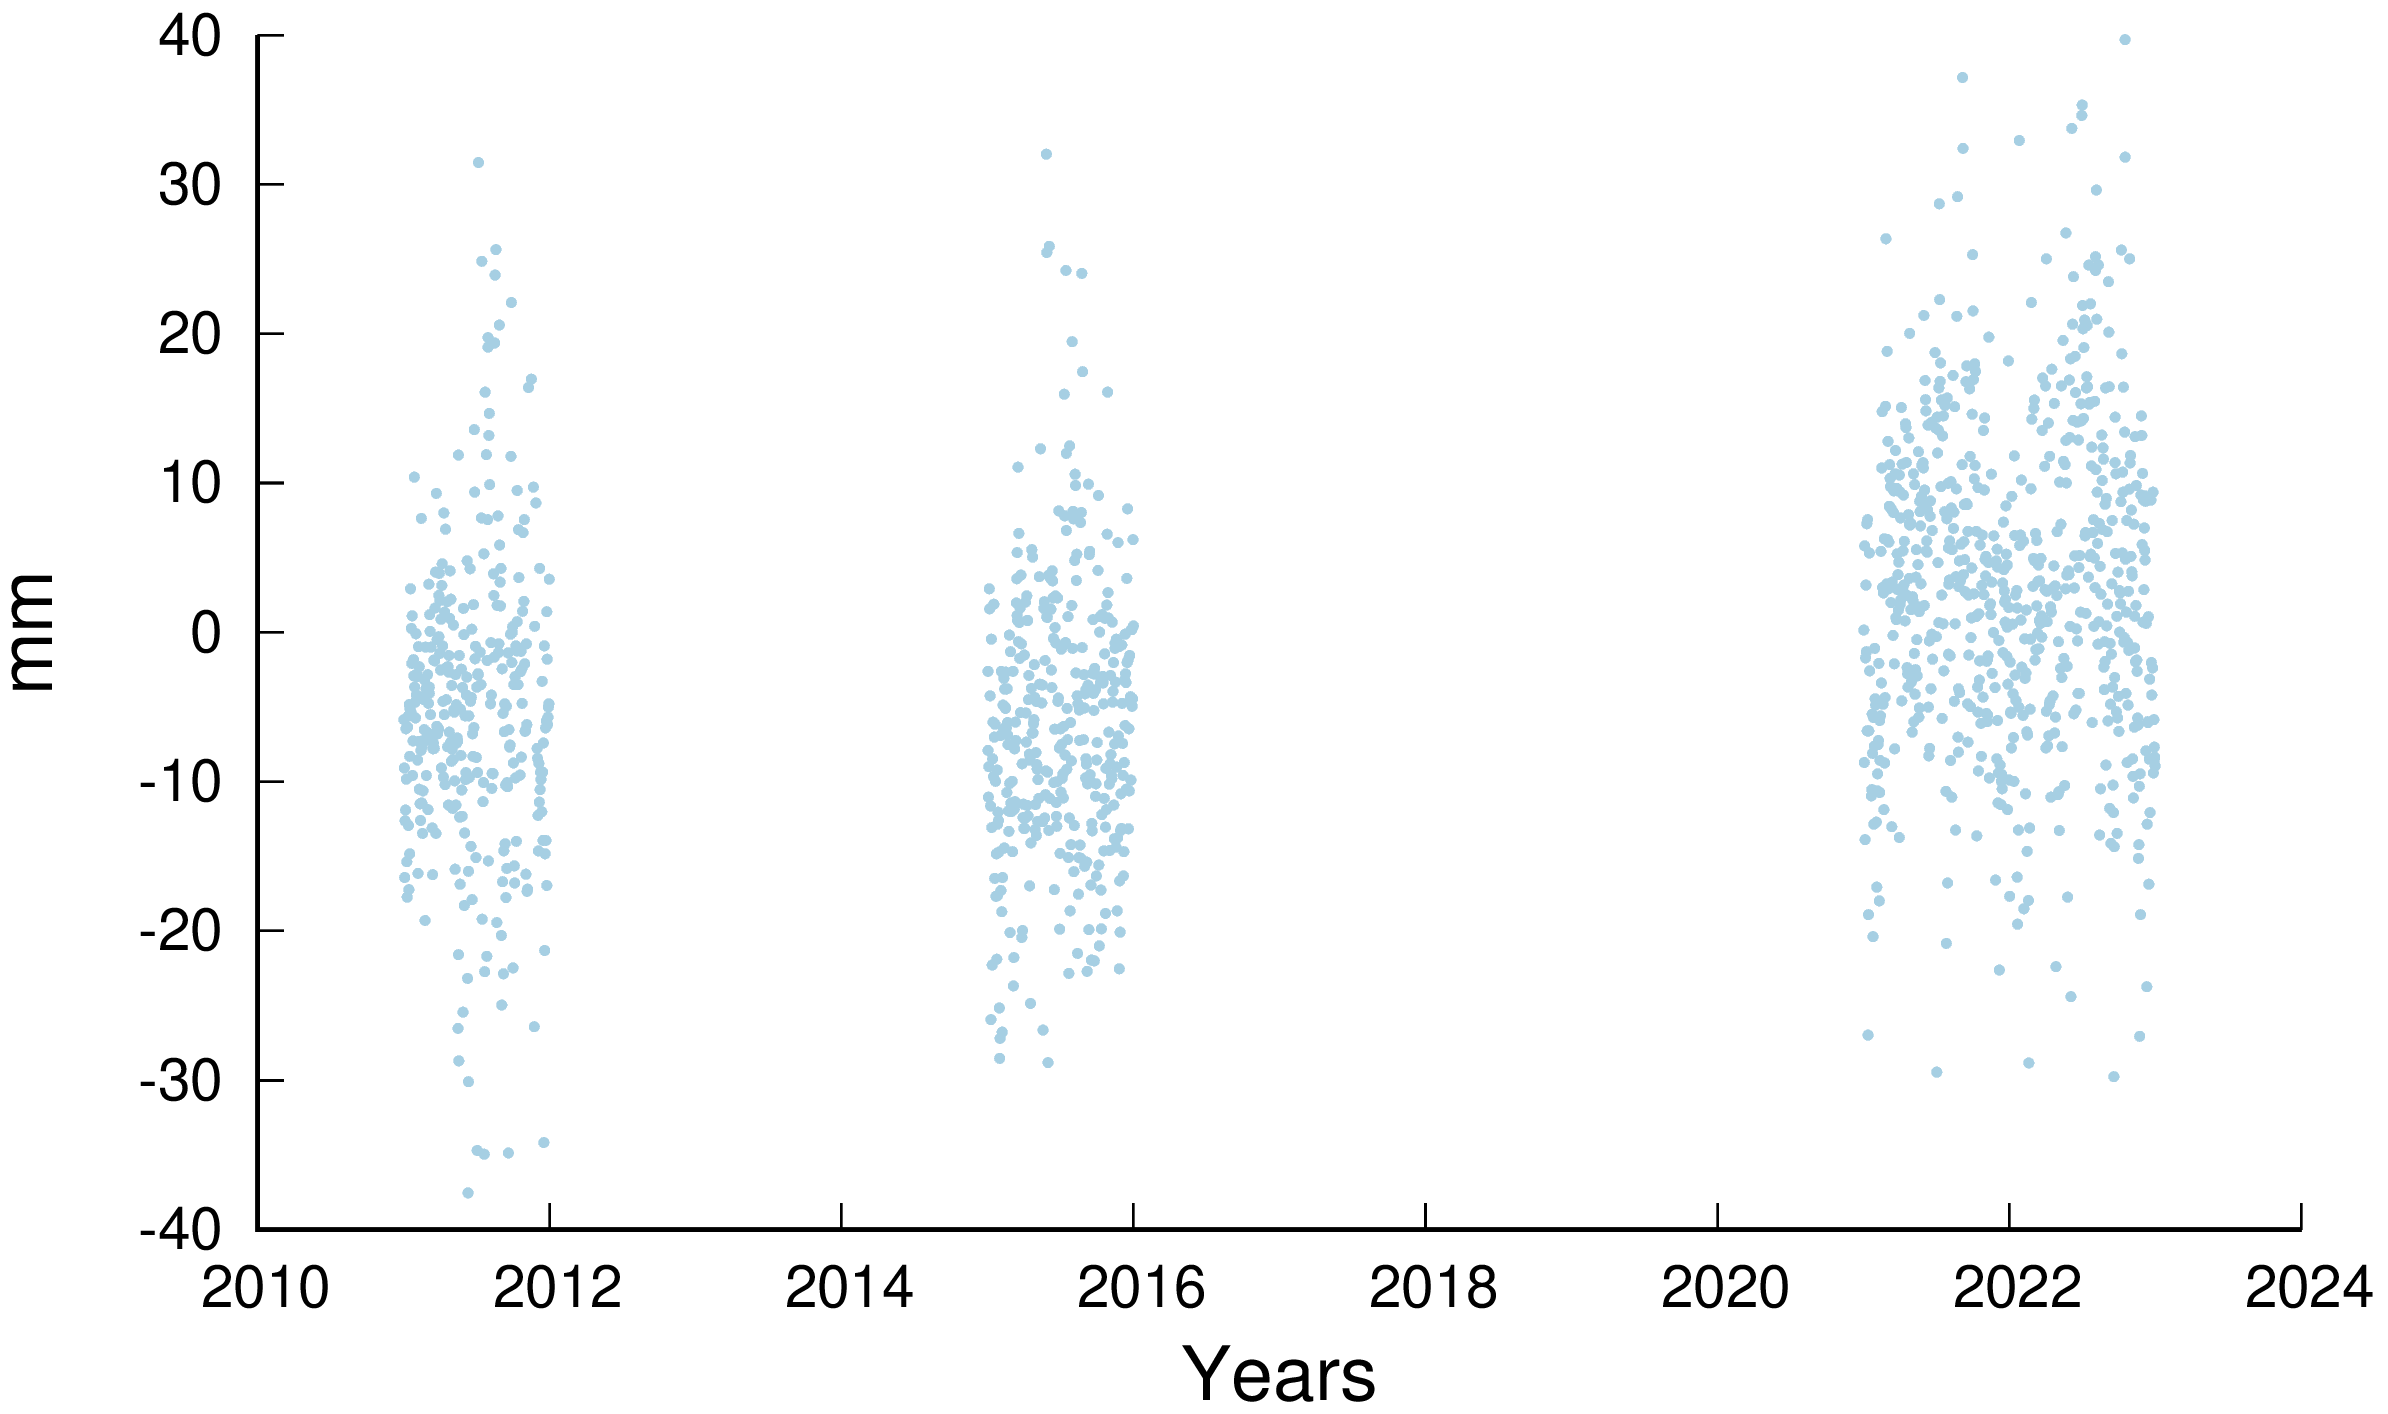
\includegraphics[width=.75\textwidth]{098a_2_data_nomodel.png}
       \end{center} 
      
    \end{column}
  \end{columns}
\end{frame}
\note{}

 % ------------------------------------------------------------------------------
\begin{frame}
  \frametitle{Συσχετισμός ασυνεχειών με σεισμούς}
  \framesubtitle{}
  \label{}
  \vskip-1cm
  \begin{columns}[T]
    \begin{column}{.33\textwidth}
      \begin{table}[H]{\small
      \begin{center}
      \begin{tabular*}{.97\linewidth}{@{\extracolsep{\fill}} c c c c}
        \toprule
         date & Δn & Δe & Δu\\
              & \multicolumn{3}{c}{(mm)}\\
        \midrule
        \multicolumn{4}{l}{Station: 040A}\\
        26.01.2014 & -43.1 & 25.2 & 2.2 \\
        17.11.2015 & -10.8 & 1.7 & 3.1\\
        \midrule
        \multicolumn{4}{l}{Station: 057A}\\
        03.03.2021 & 47.9 & 27.6 & 14.0\\
        \bottomrule
      \end{tabular*}
      \end{center}}
      \end{table}
    \end{column}
    \begin{column}{.33\textwidth}
      \begin{center}
      Station:\textbf{040A}\\
         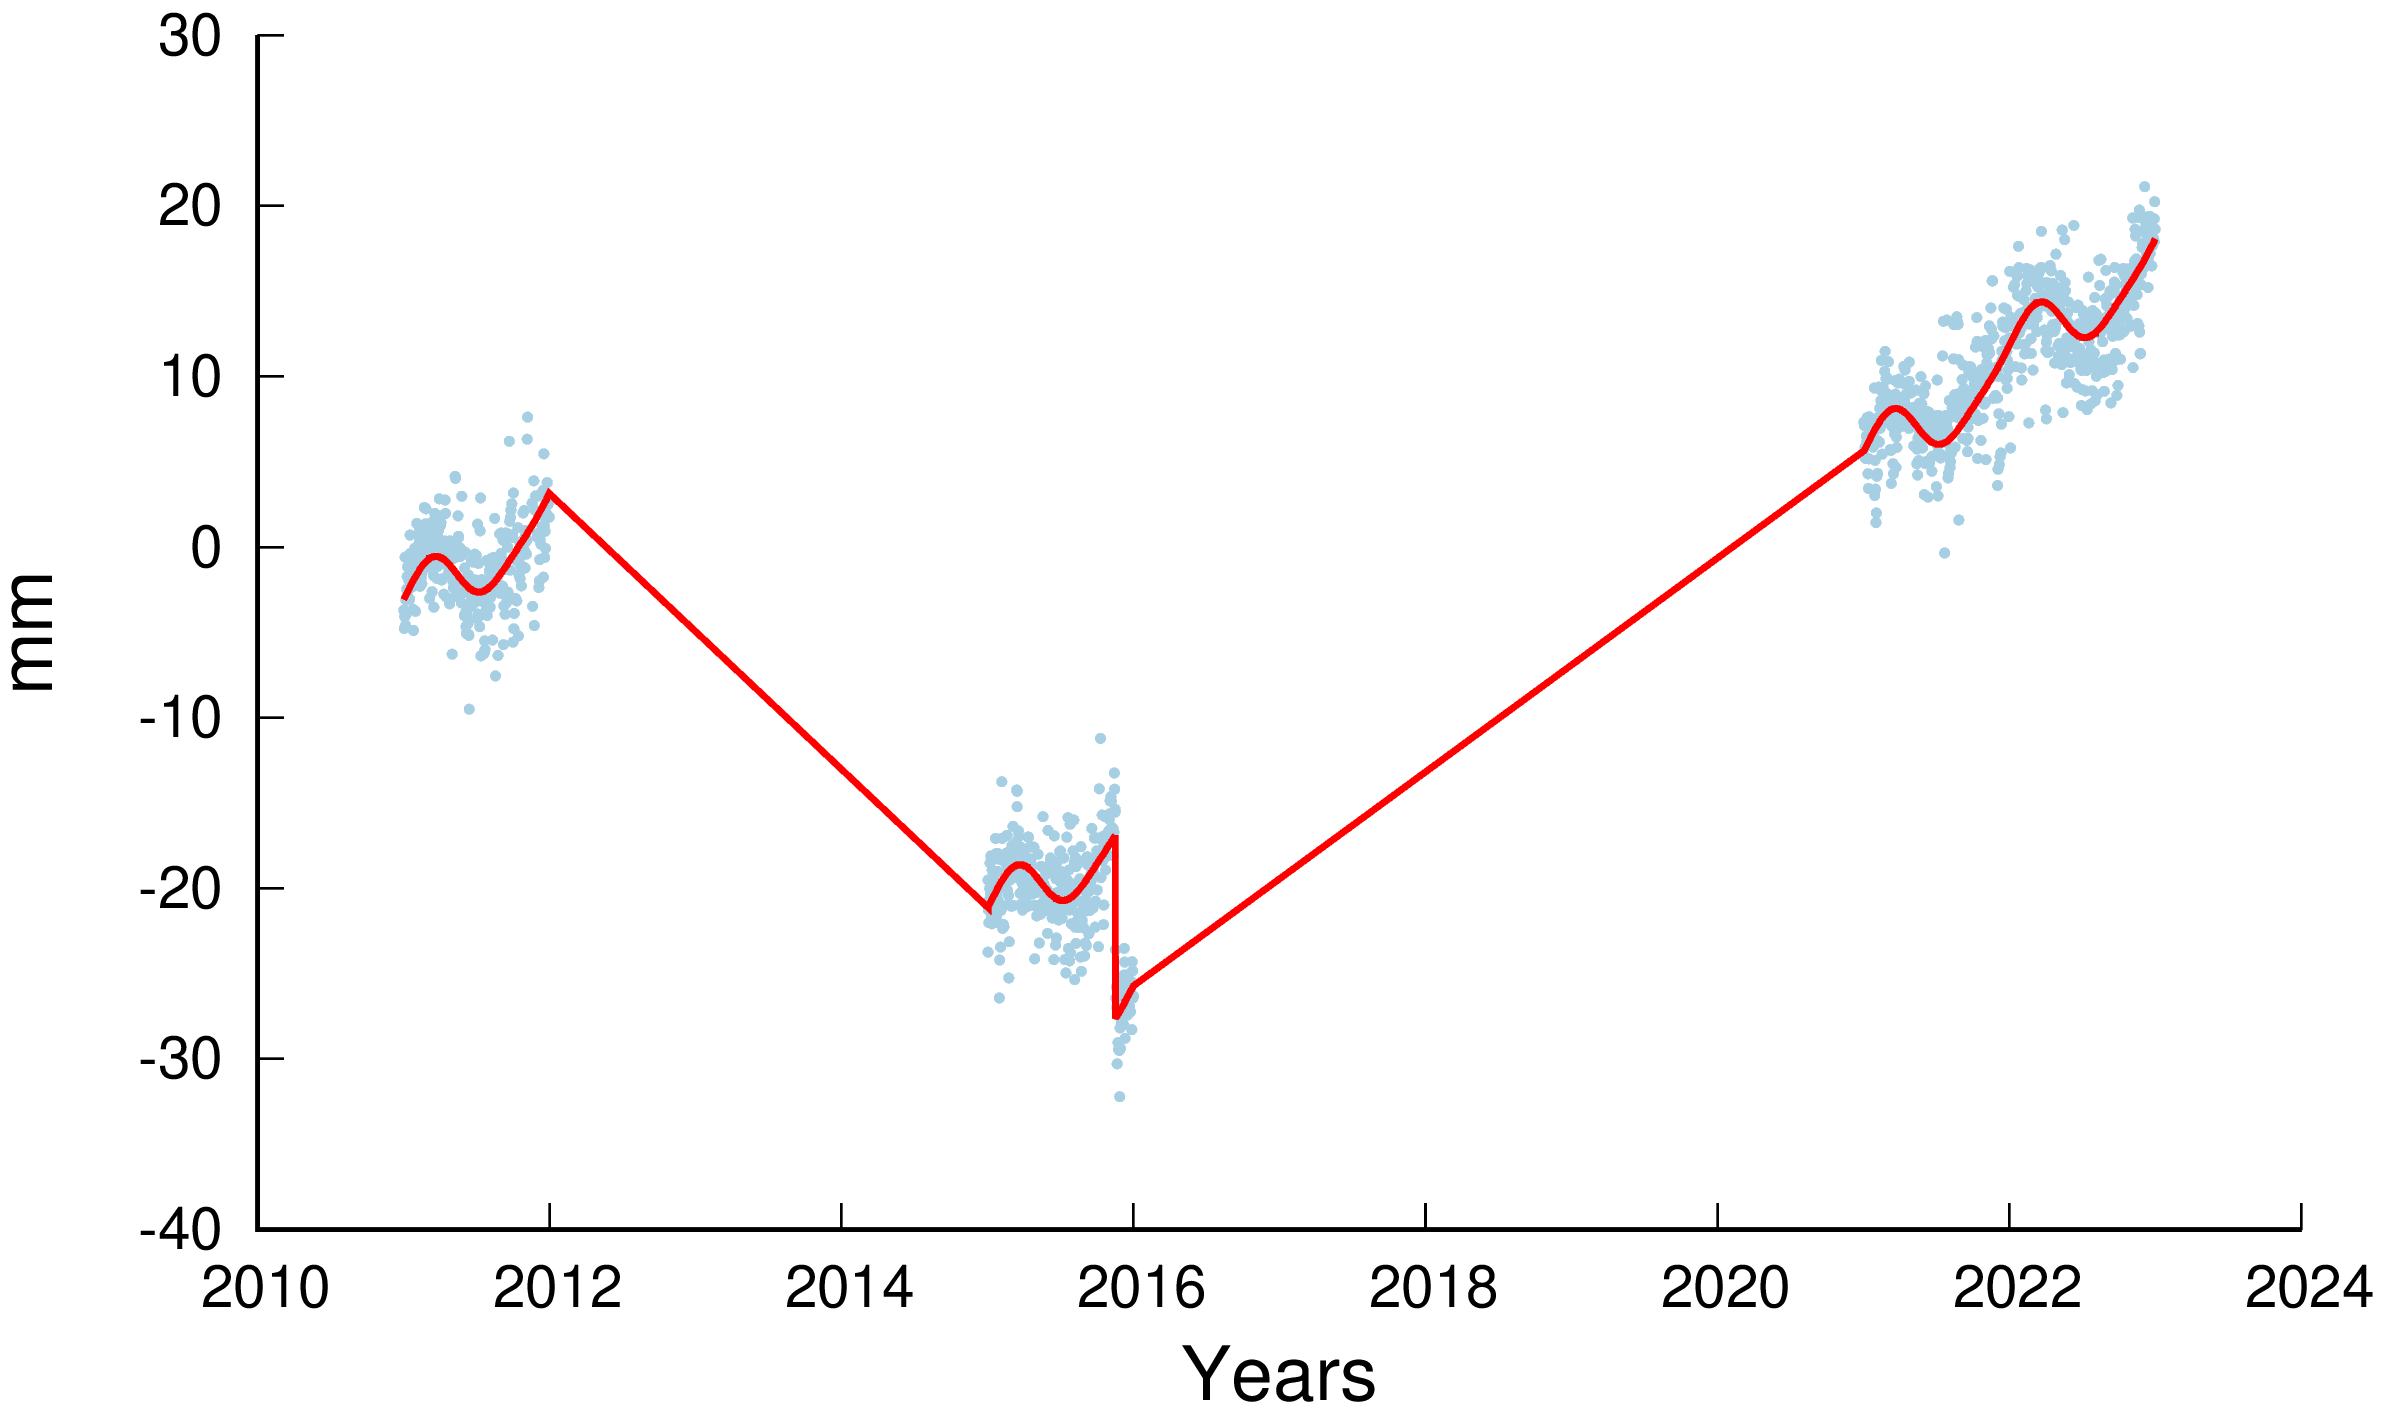
\includegraphics[width=.75\textwidth]{040a_0_data.png}\\
         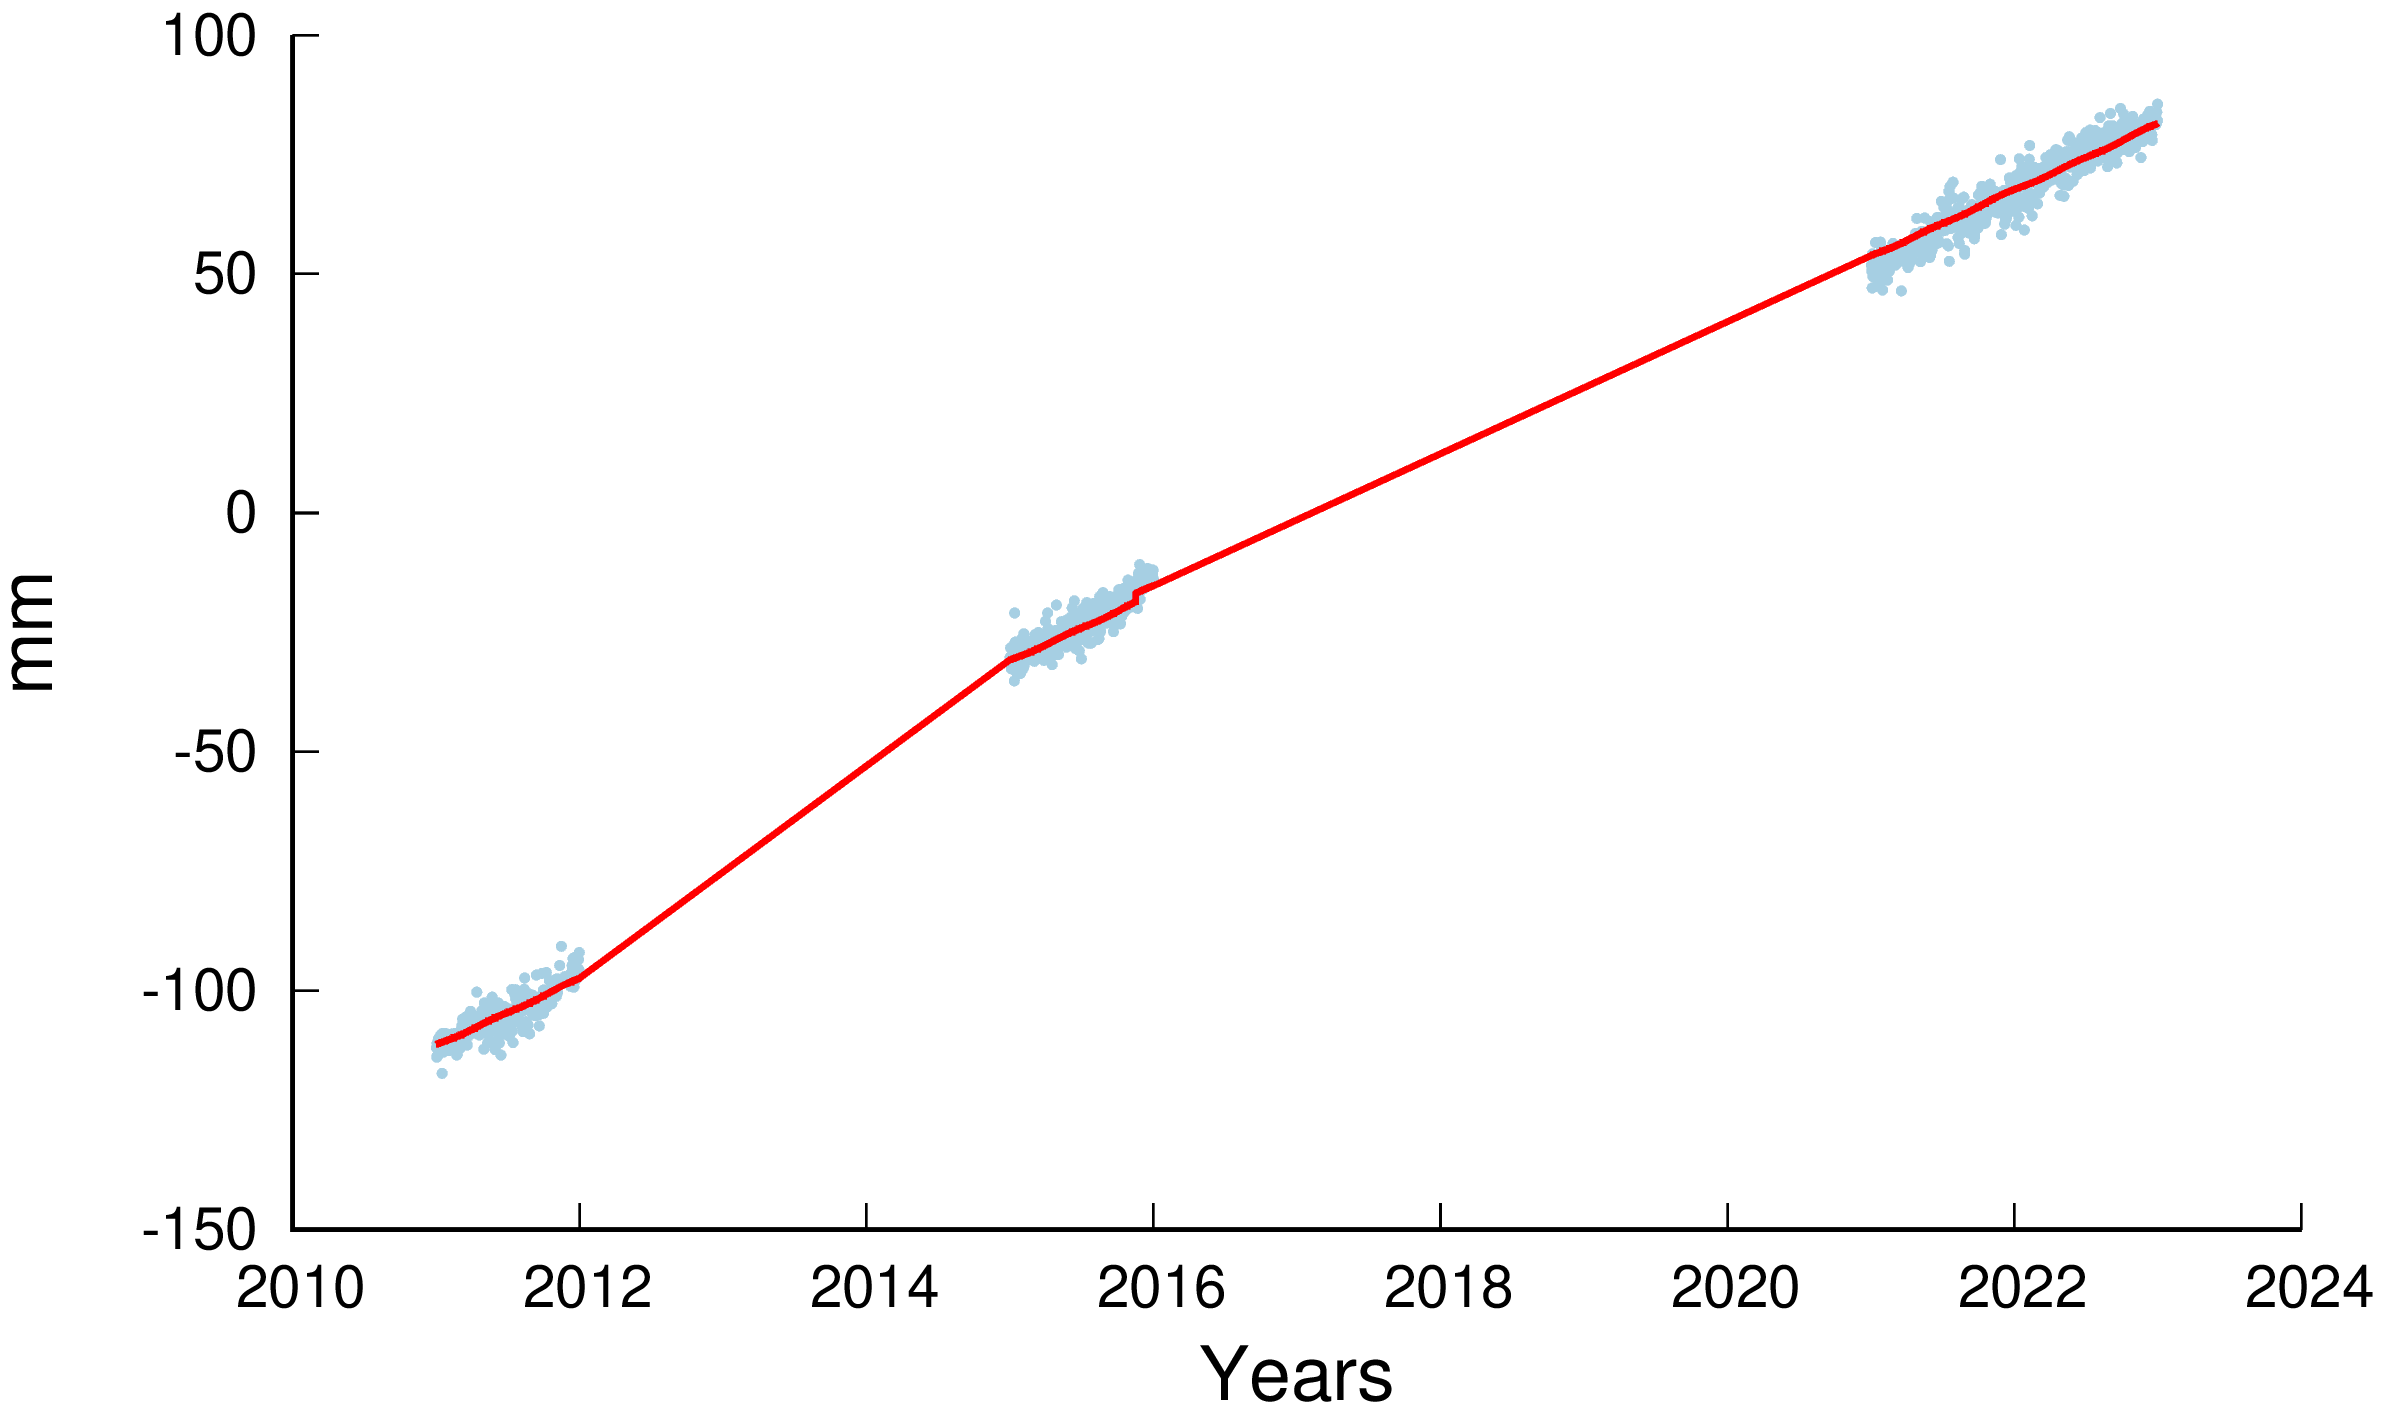
\includegraphics[width=.75\textwidth]{040a_1_data.png}\\
         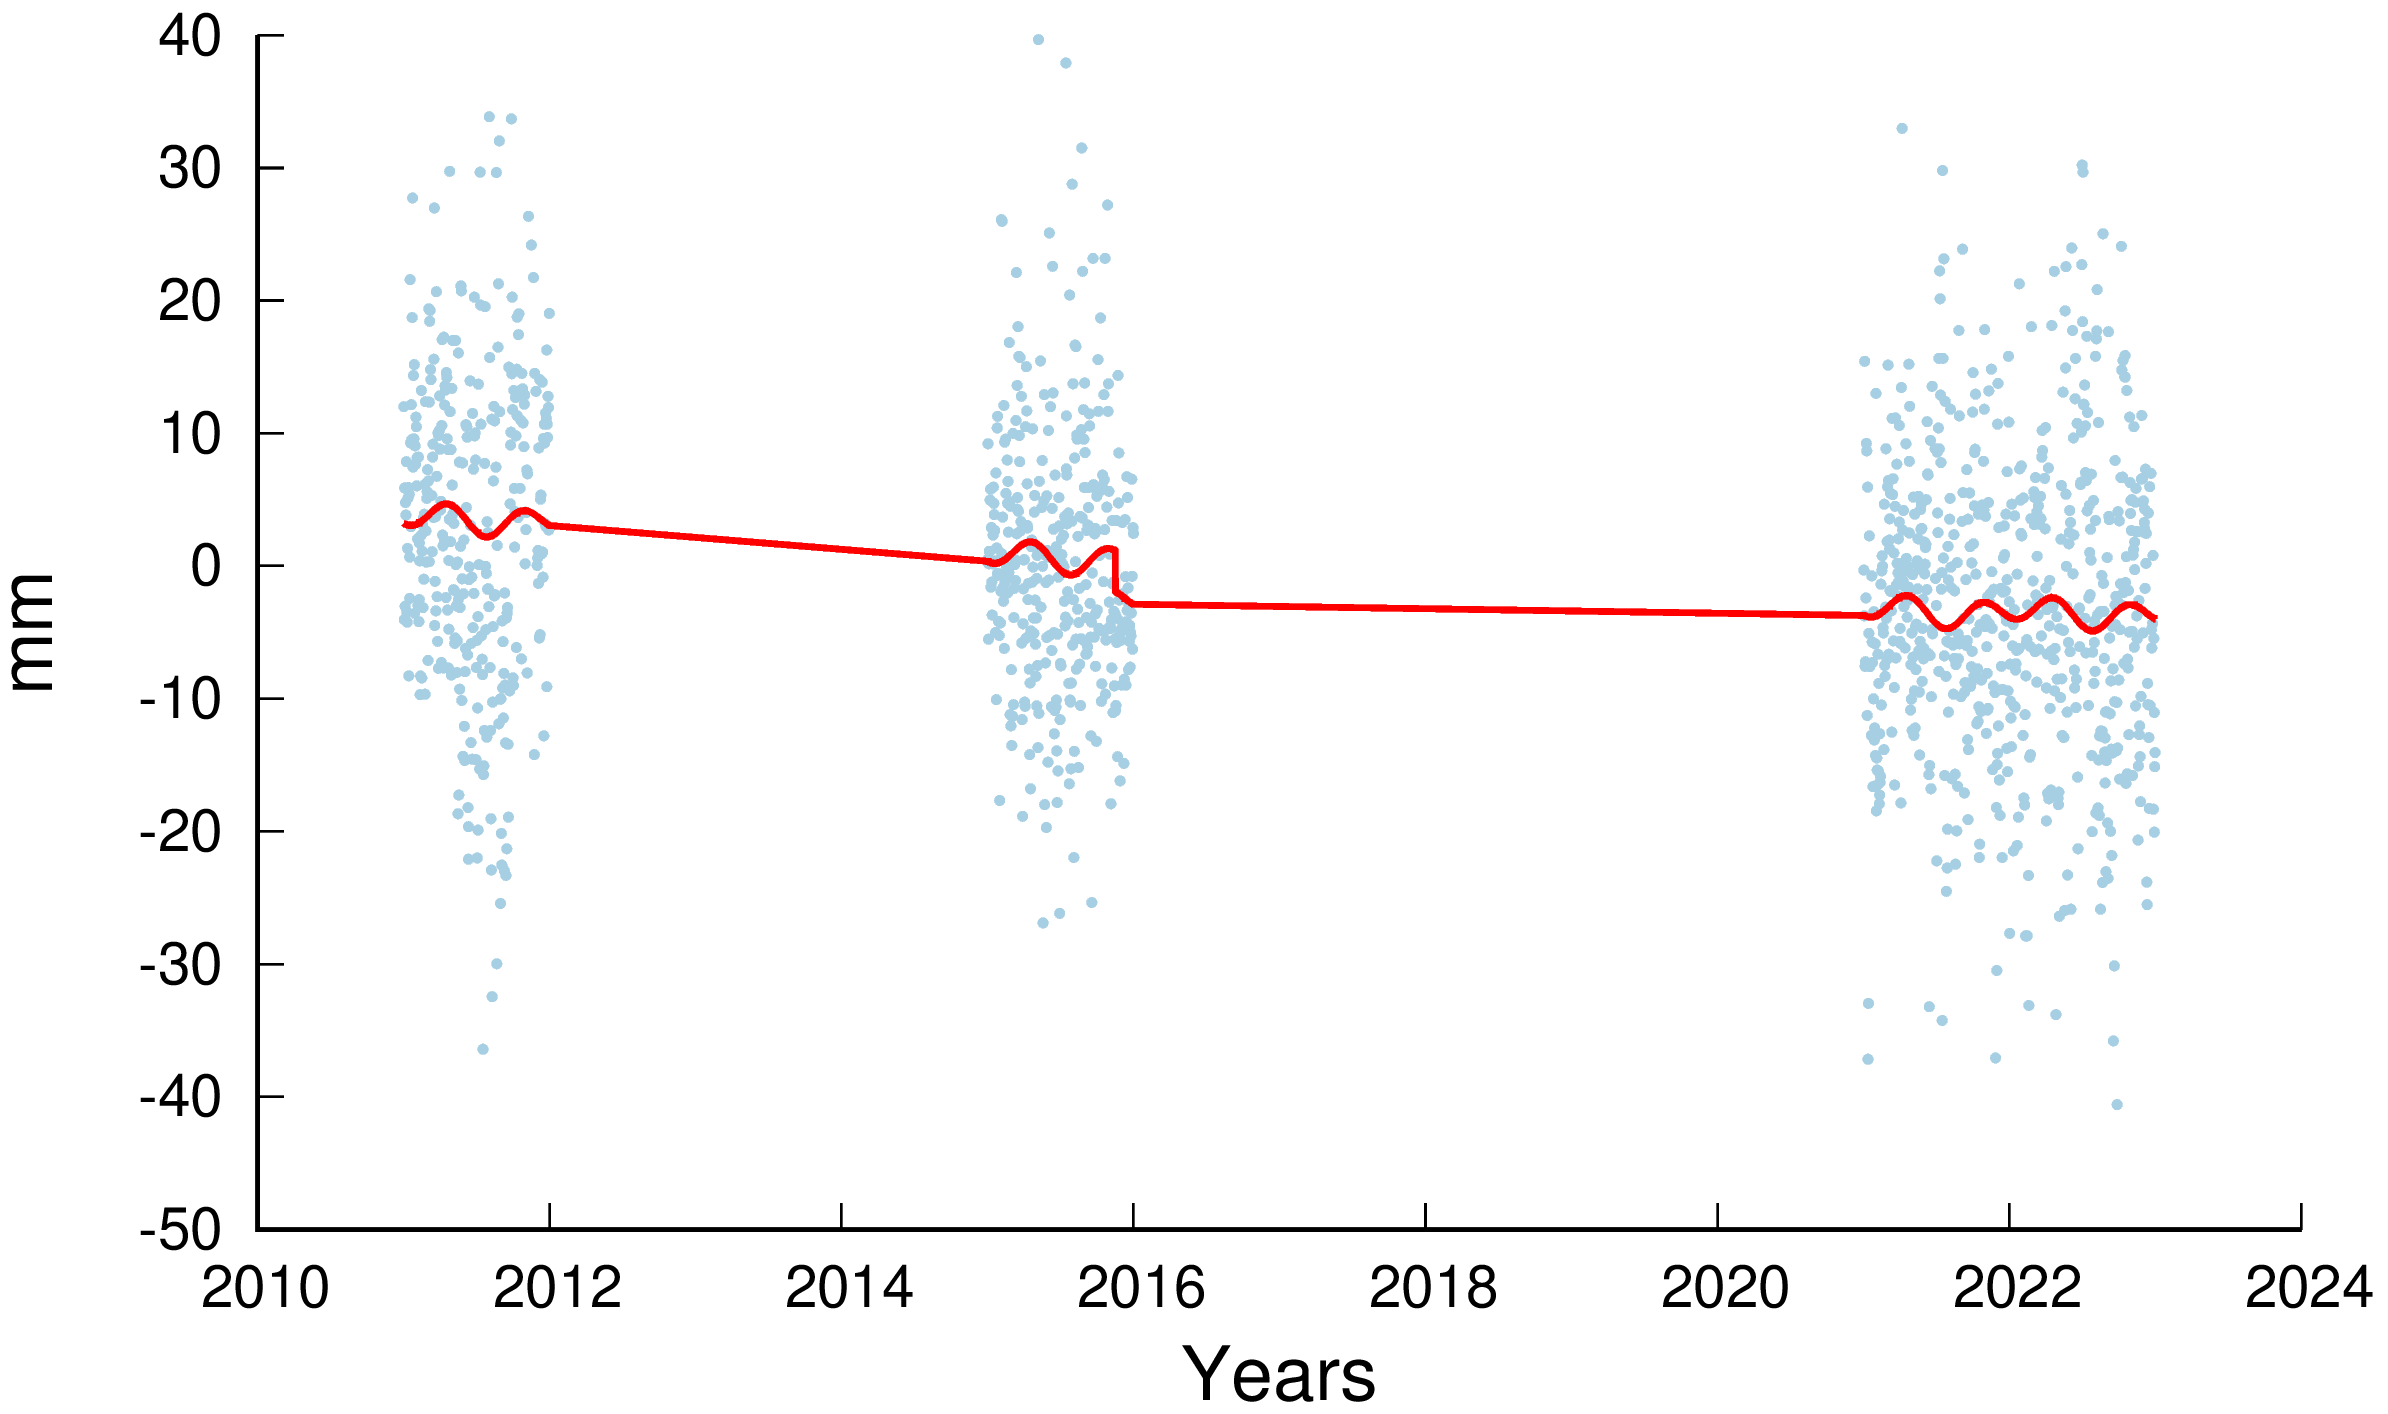
\includegraphics[width=.75\textwidth]{040a_2_data.png}
       \end{center} 
    \end{column}
    \begin{column}{.33\textwidth}
      \begin{center}
      Station:\textbf{057A}\\
         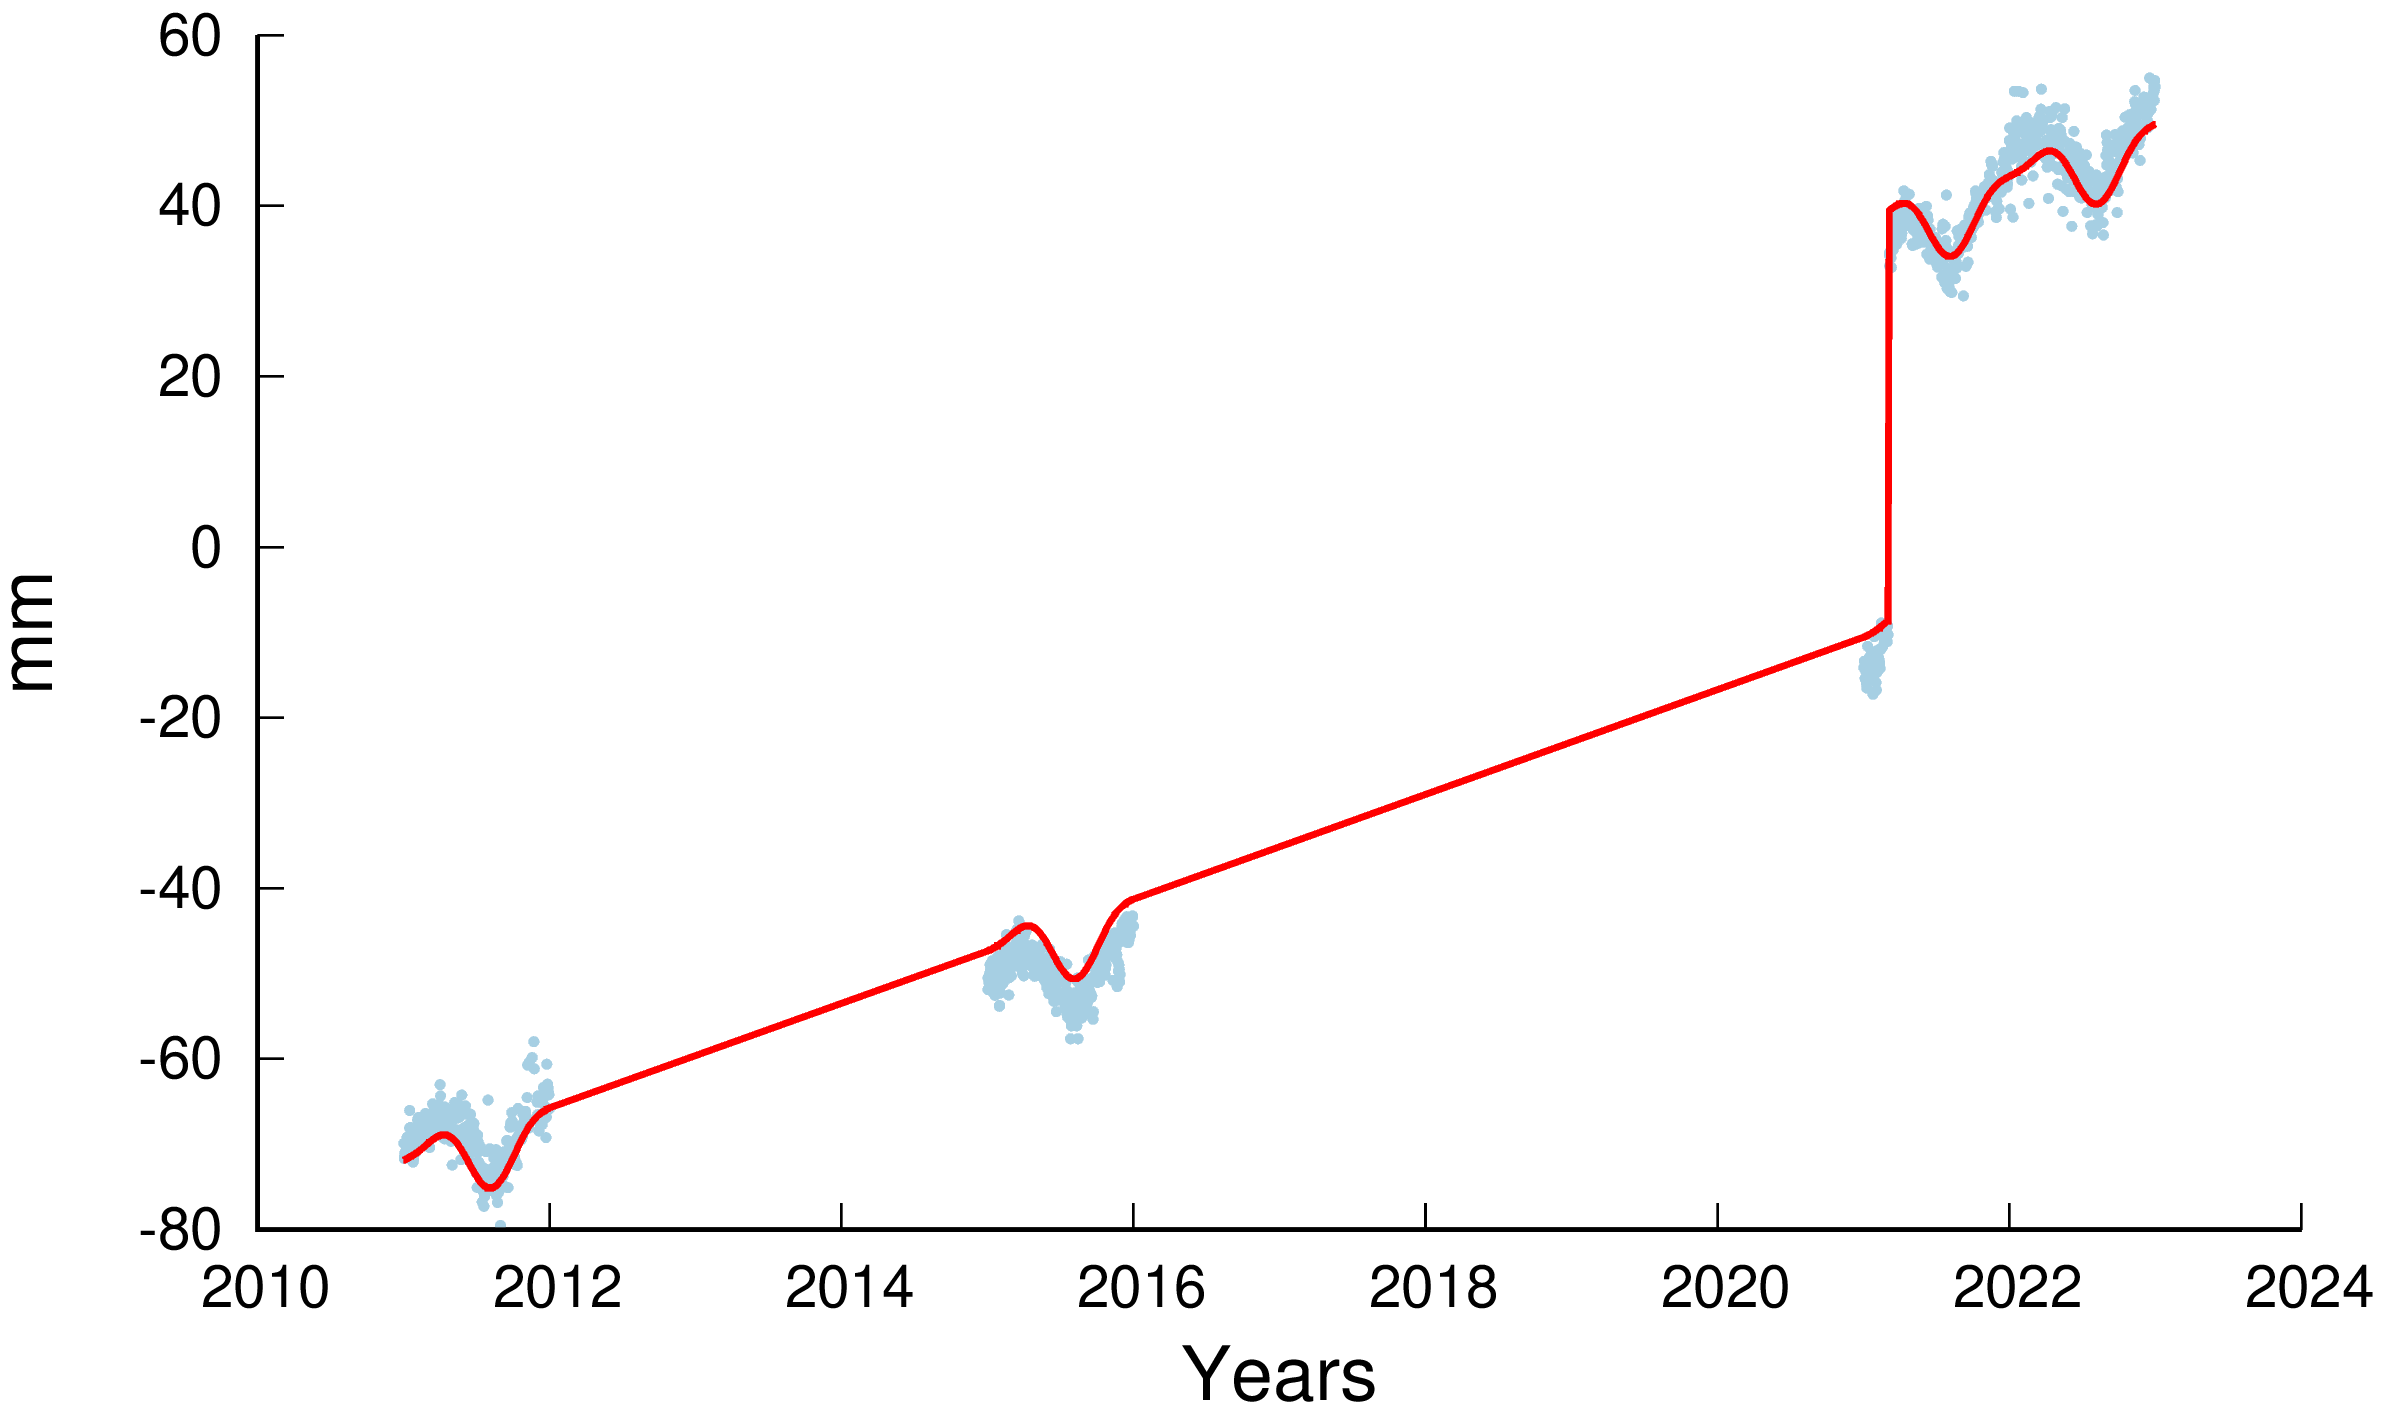
\includegraphics[width=.75\textwidth]{057a_0_data.png}\\
         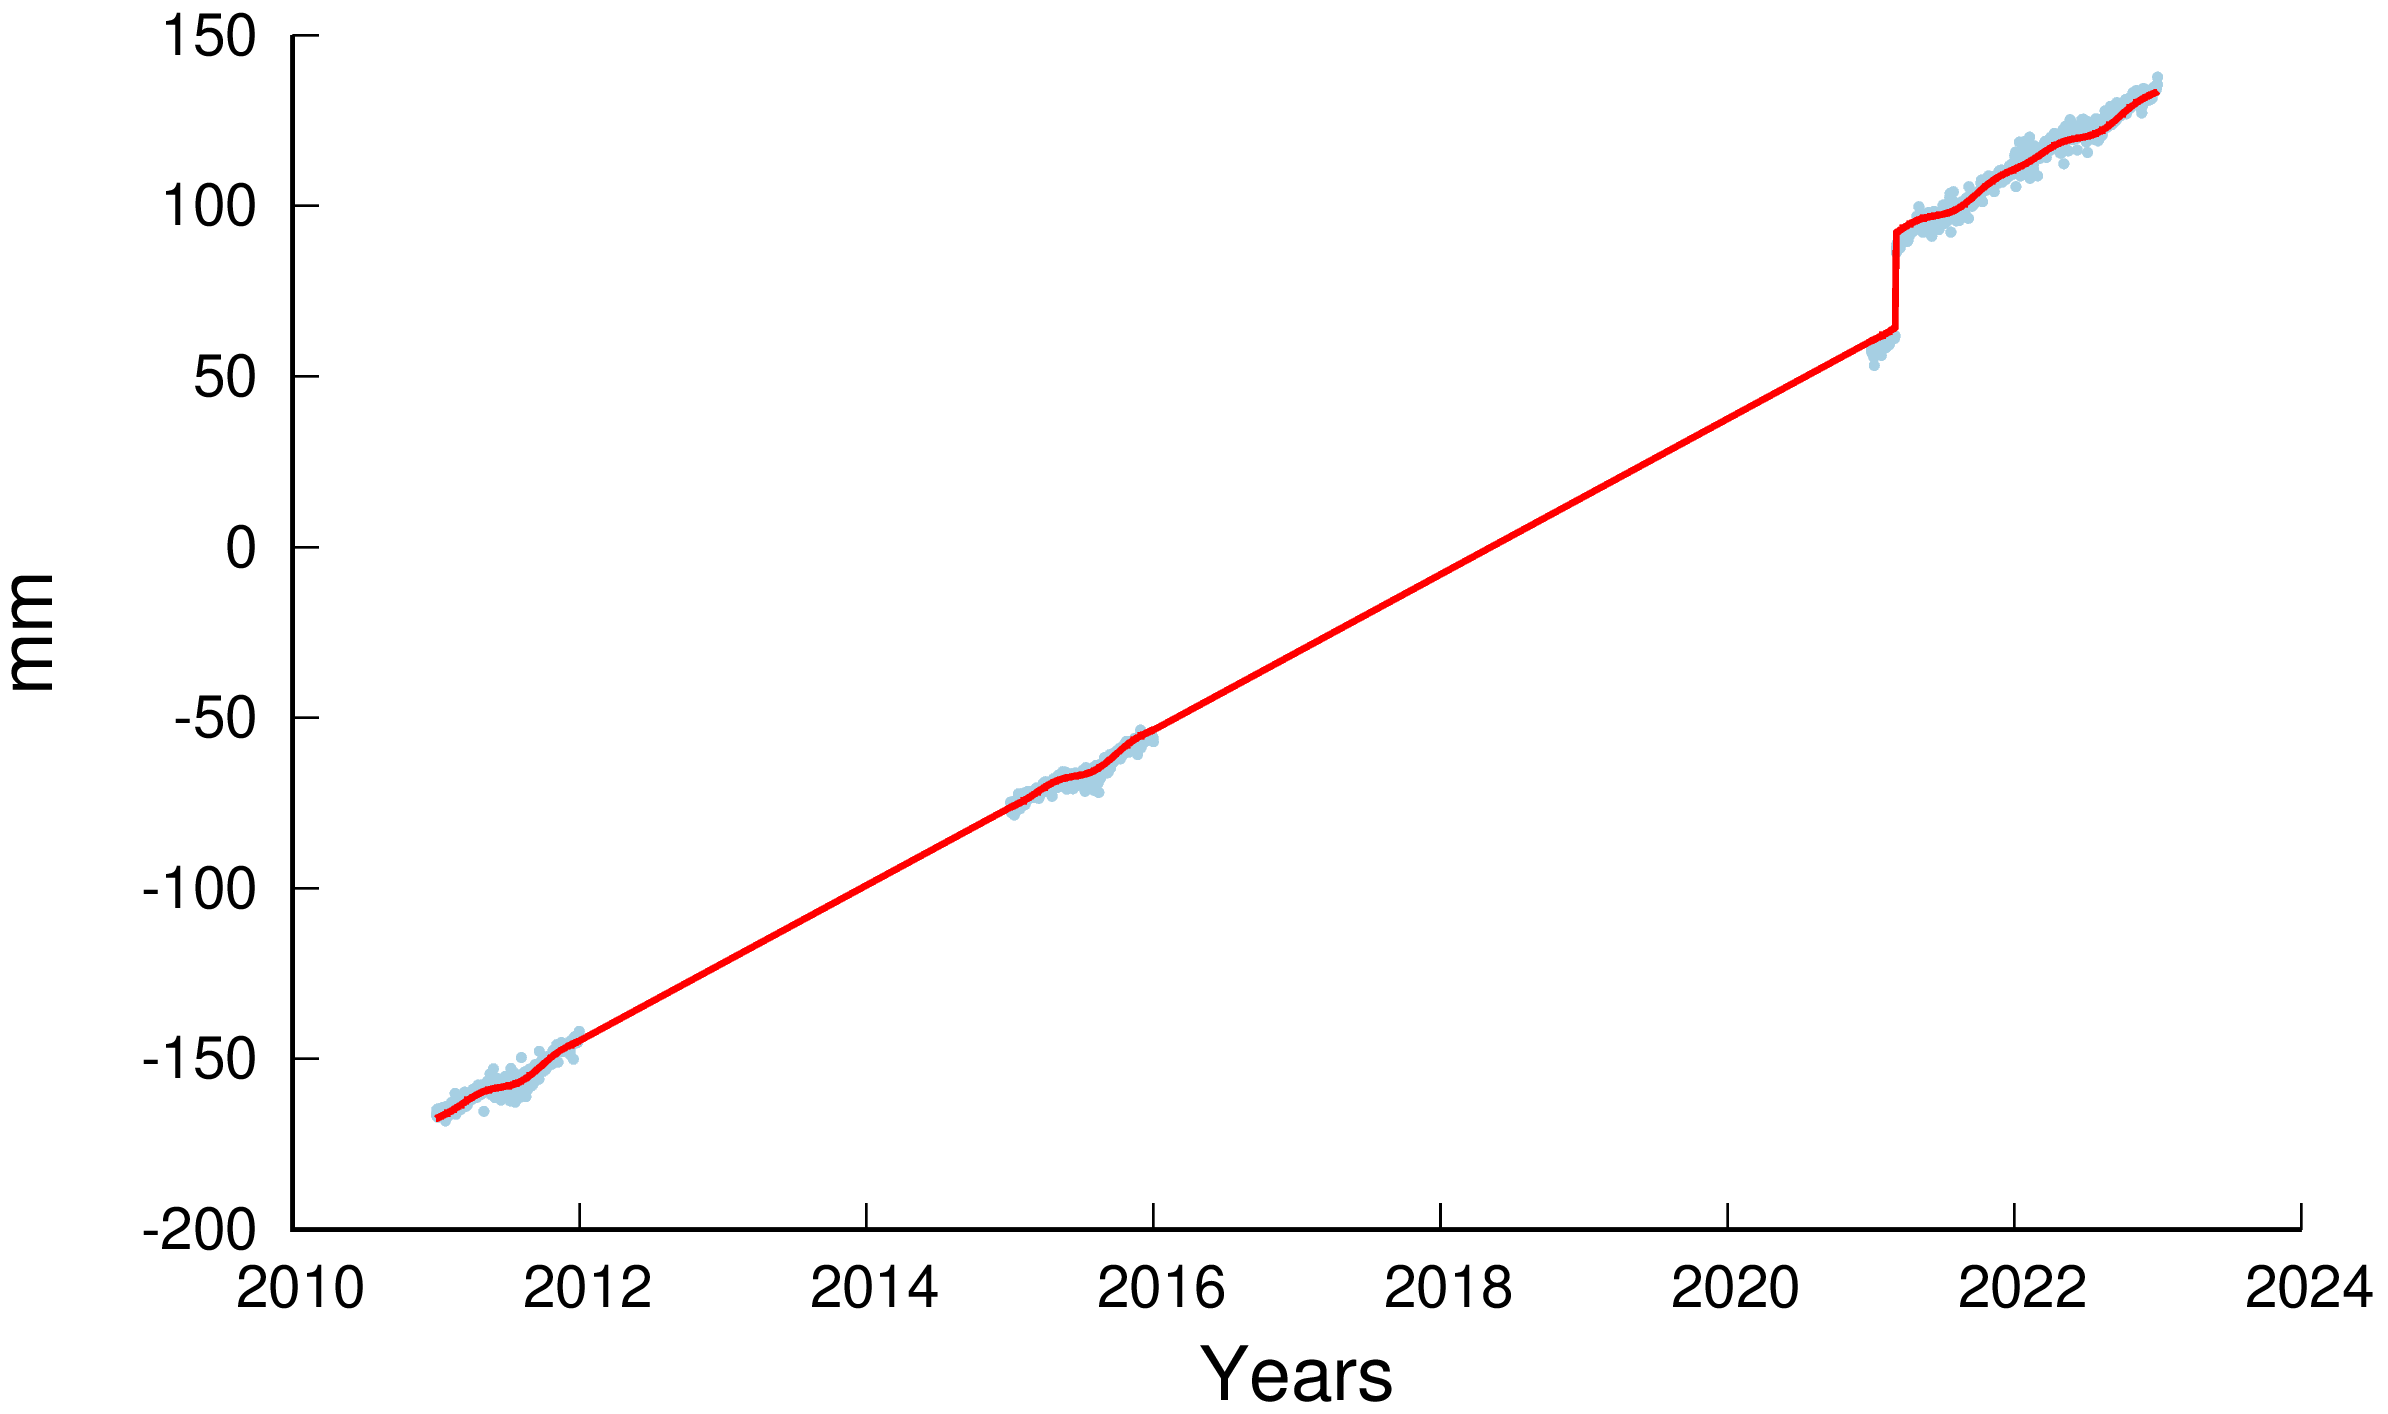
\includegraphics[width=.75\textwidth]{057a_1_data.png}\\
         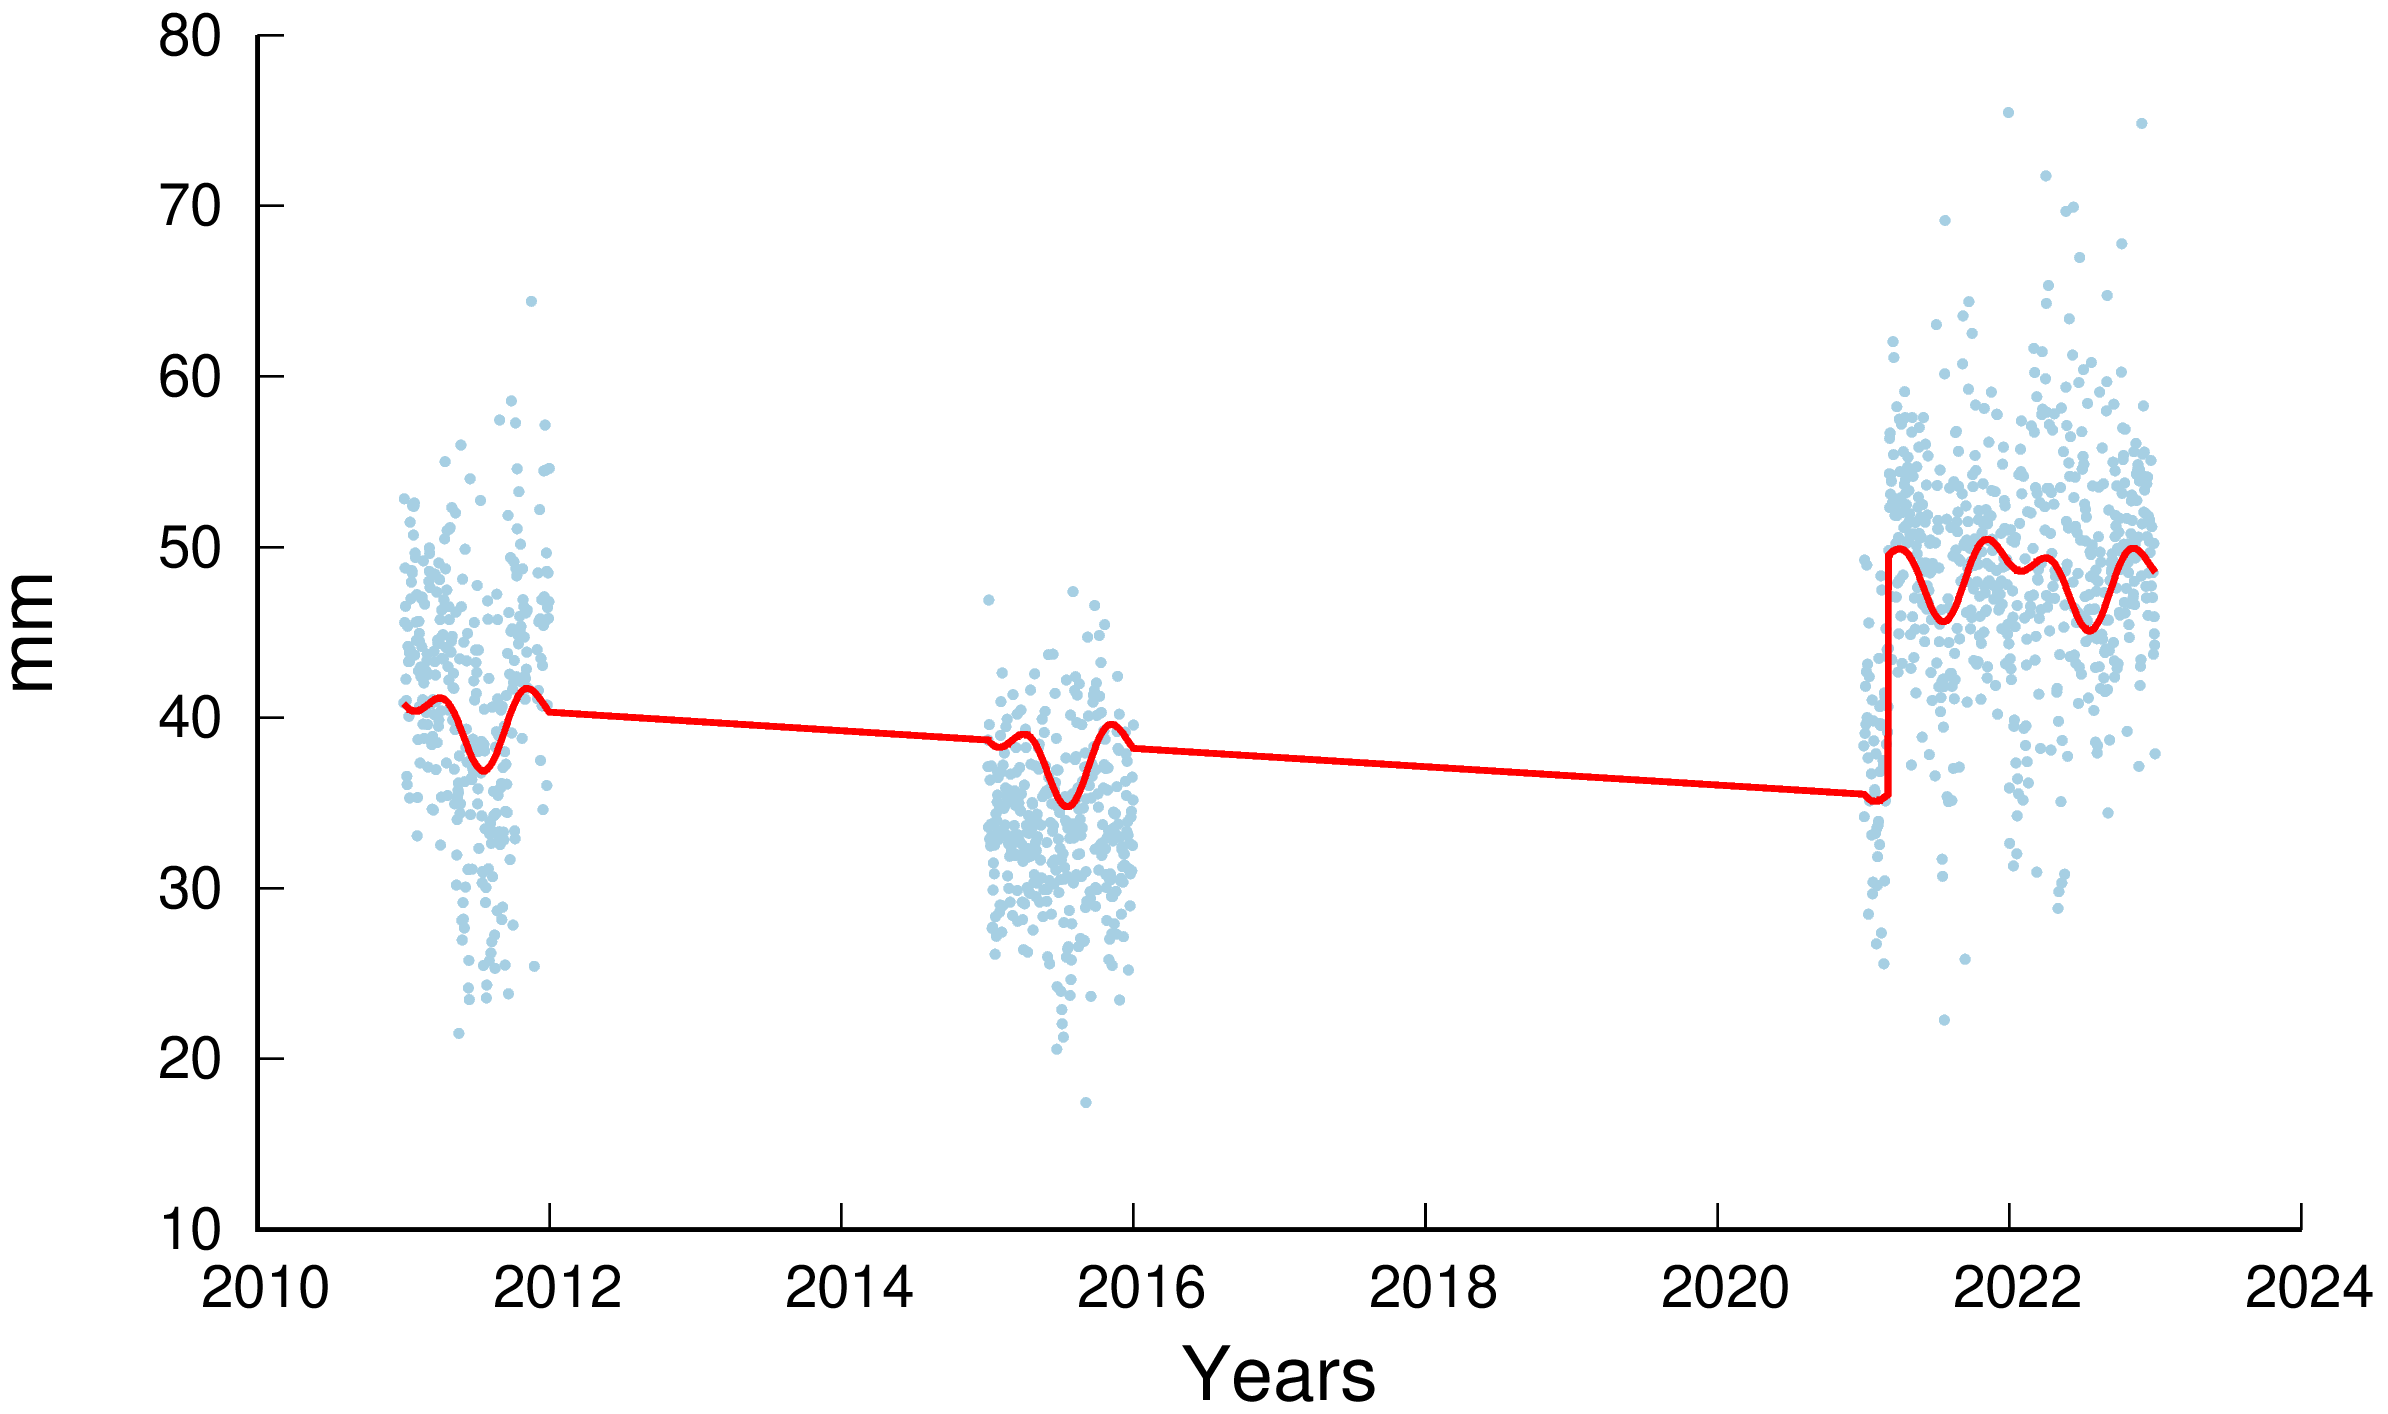
\includegraphics[width=.75\textwidth]{057a_2_data.png}
       \end{center} 
    \end{column}
  \end{columns}
\end{frame}
\note{}

 % ------------------------------------------------------------------------------
\begin{frame}
  \frametitle{Αρμονική ανάλυση}
  \framesubtitle{}
  \label{}
  \vskip-1cm
  \begin{columns}[T]
    \begin{column}{.33\textwidth}
      \begin{align*}
        \sum_{i=0}^{n_F} s_{i} sin(\omega_{i}t) + c_{i} cos(\omega_{i}t)
      \end{align*}
      Παράδειγμα αποτελεσμάτων:
       \begin{center}
         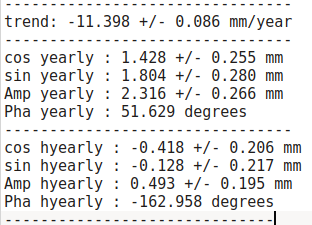
\includegraphics[width=.8\textwidth]{098a_0_lsfout.png}
       \end{center}
    \end{column}
    \begin{column}{.33\textwidth}
      \begin{center}
      Station:\textbf{040A}\\
         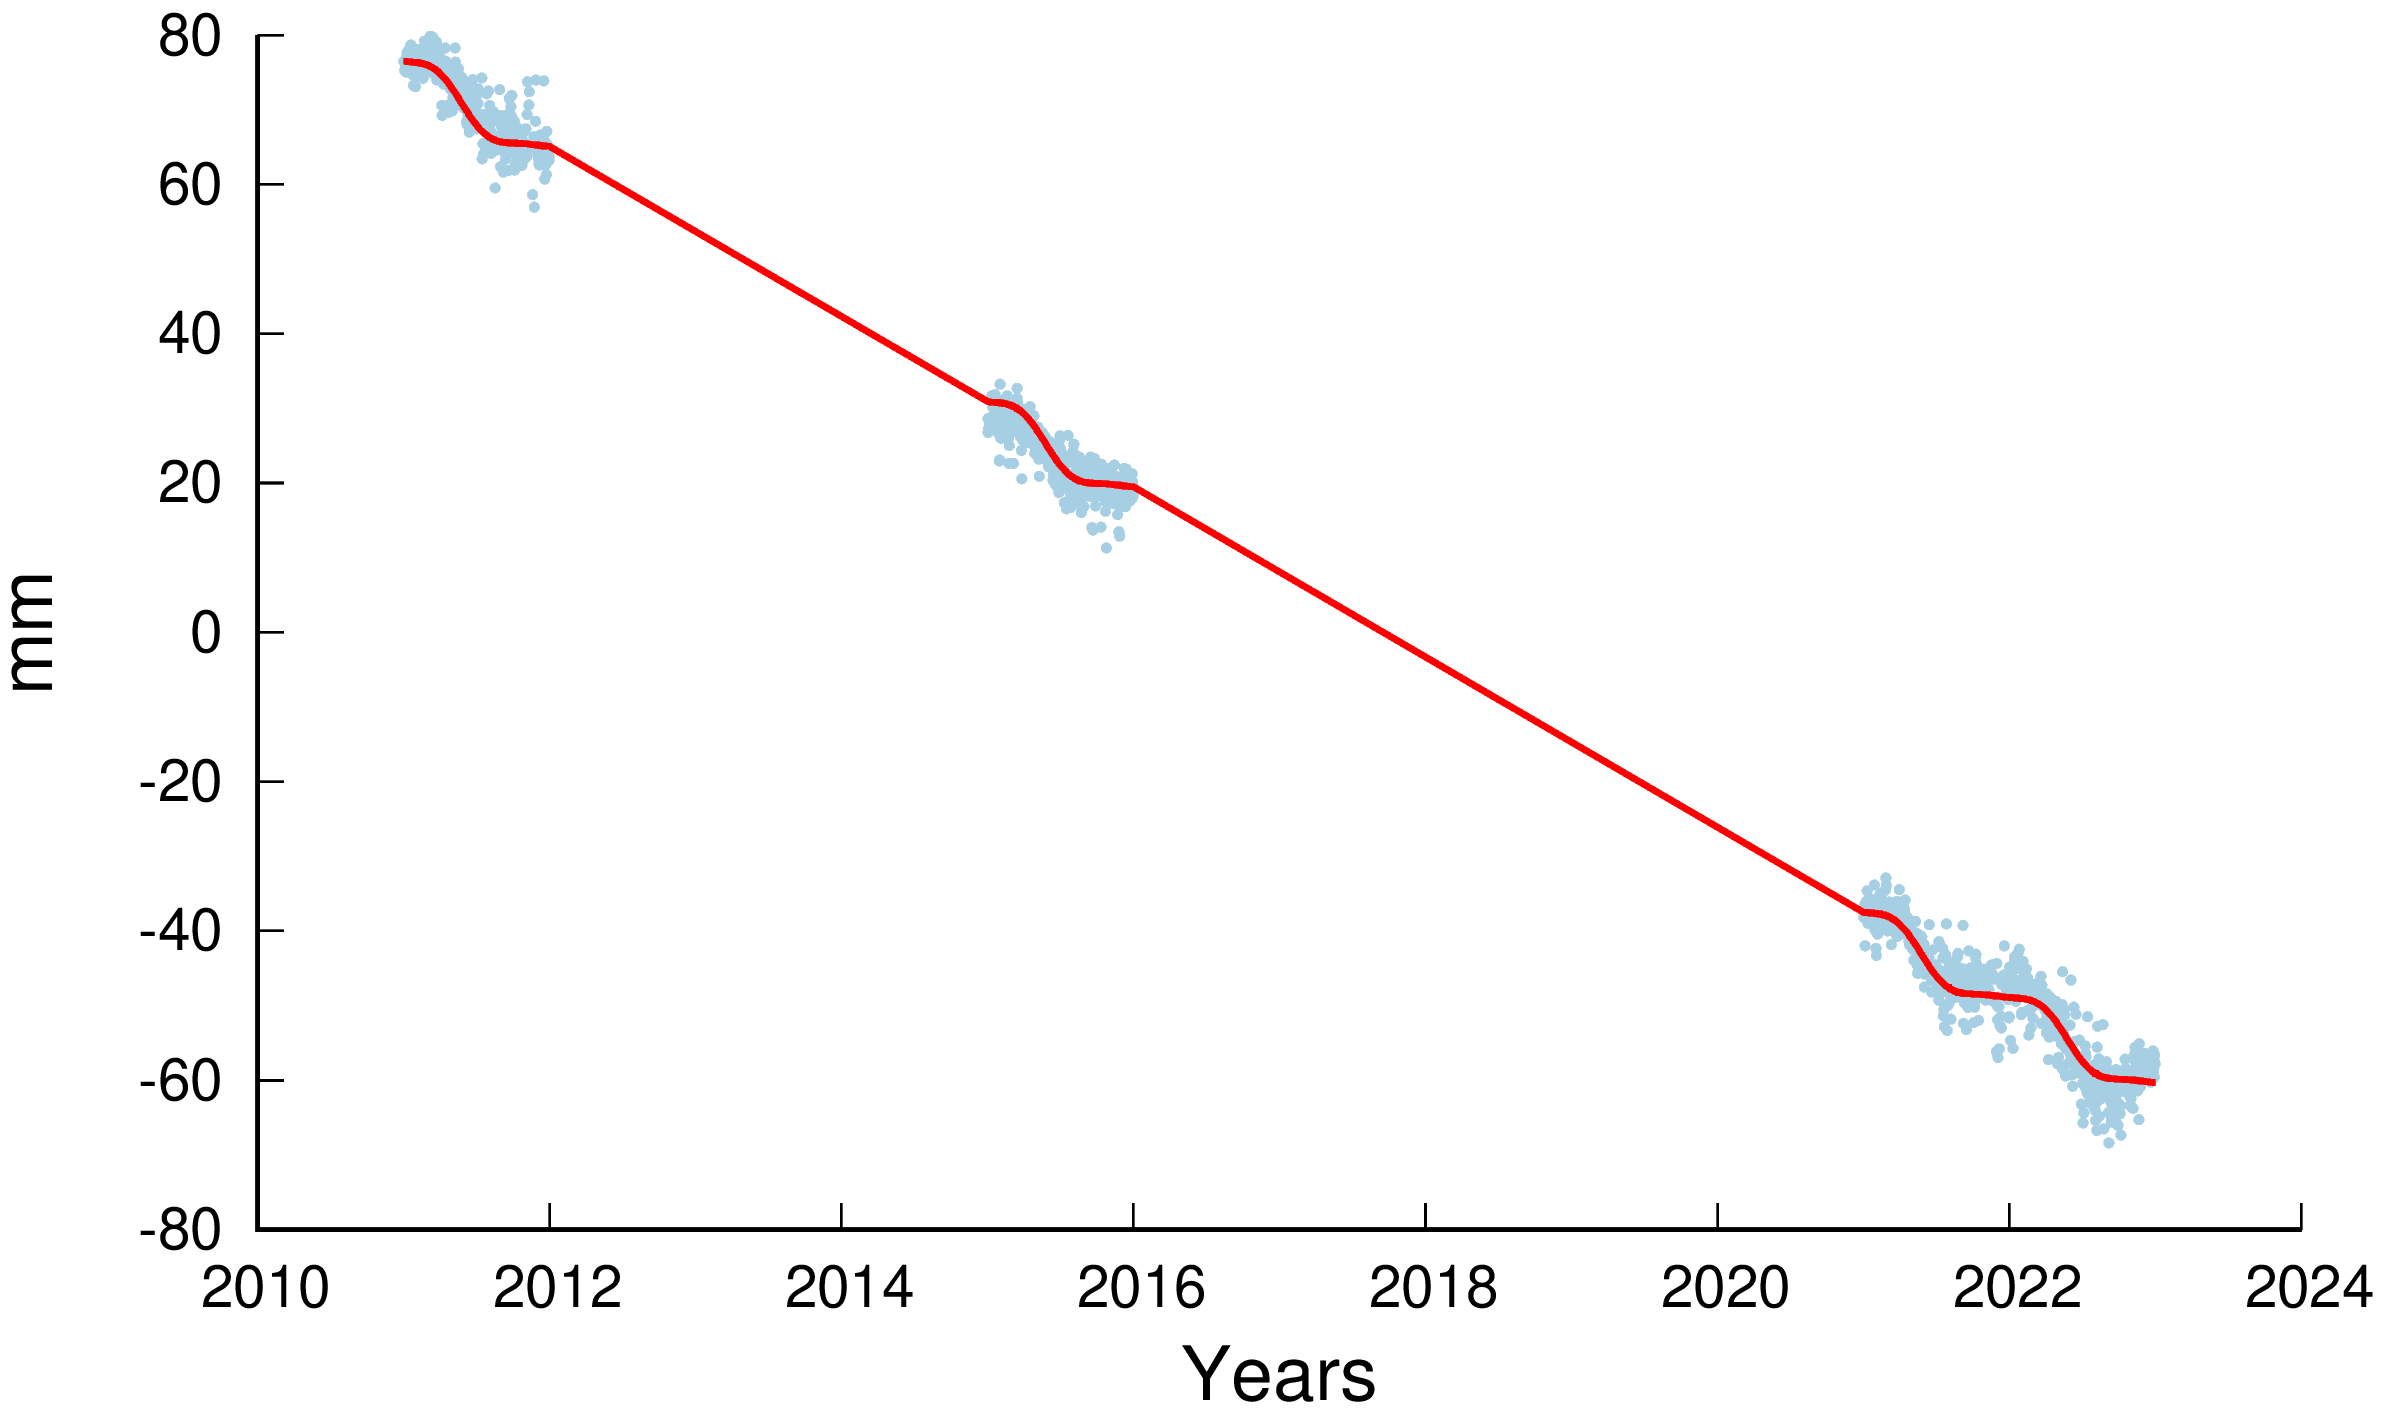
\includegraphics[width=.75\textwidth]{098a_0_data.png}\\
         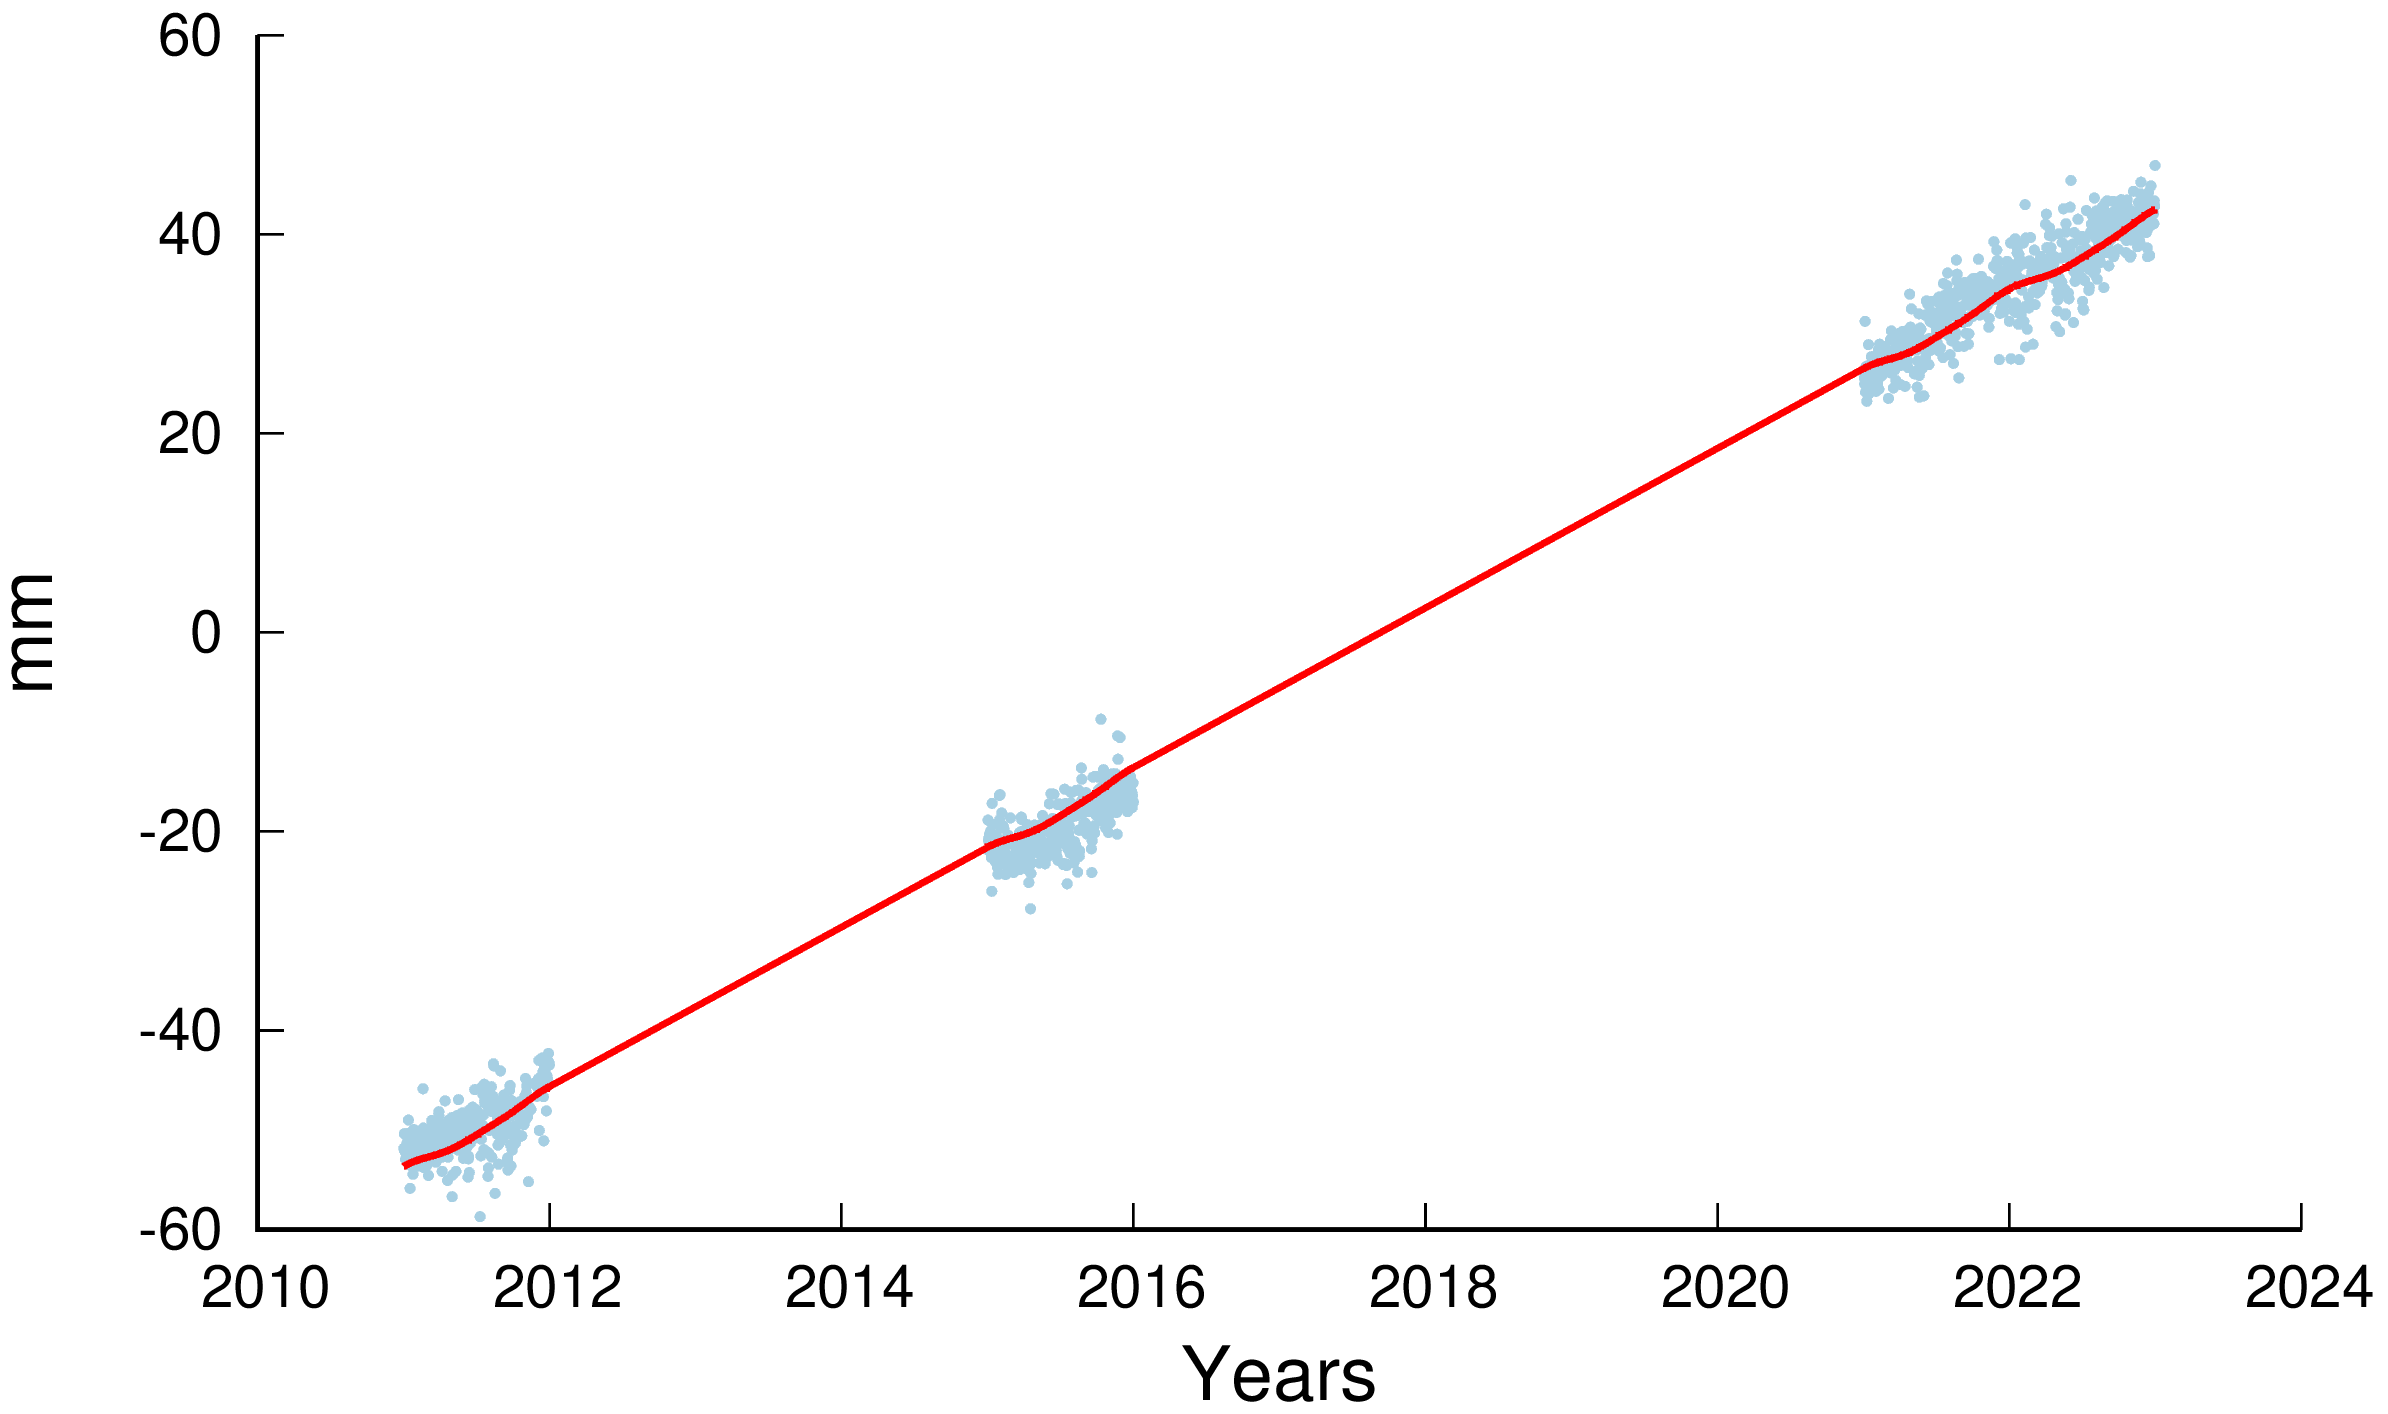
\includegraphics[width=.75\textwidth]{098a_1_data.png}\\
         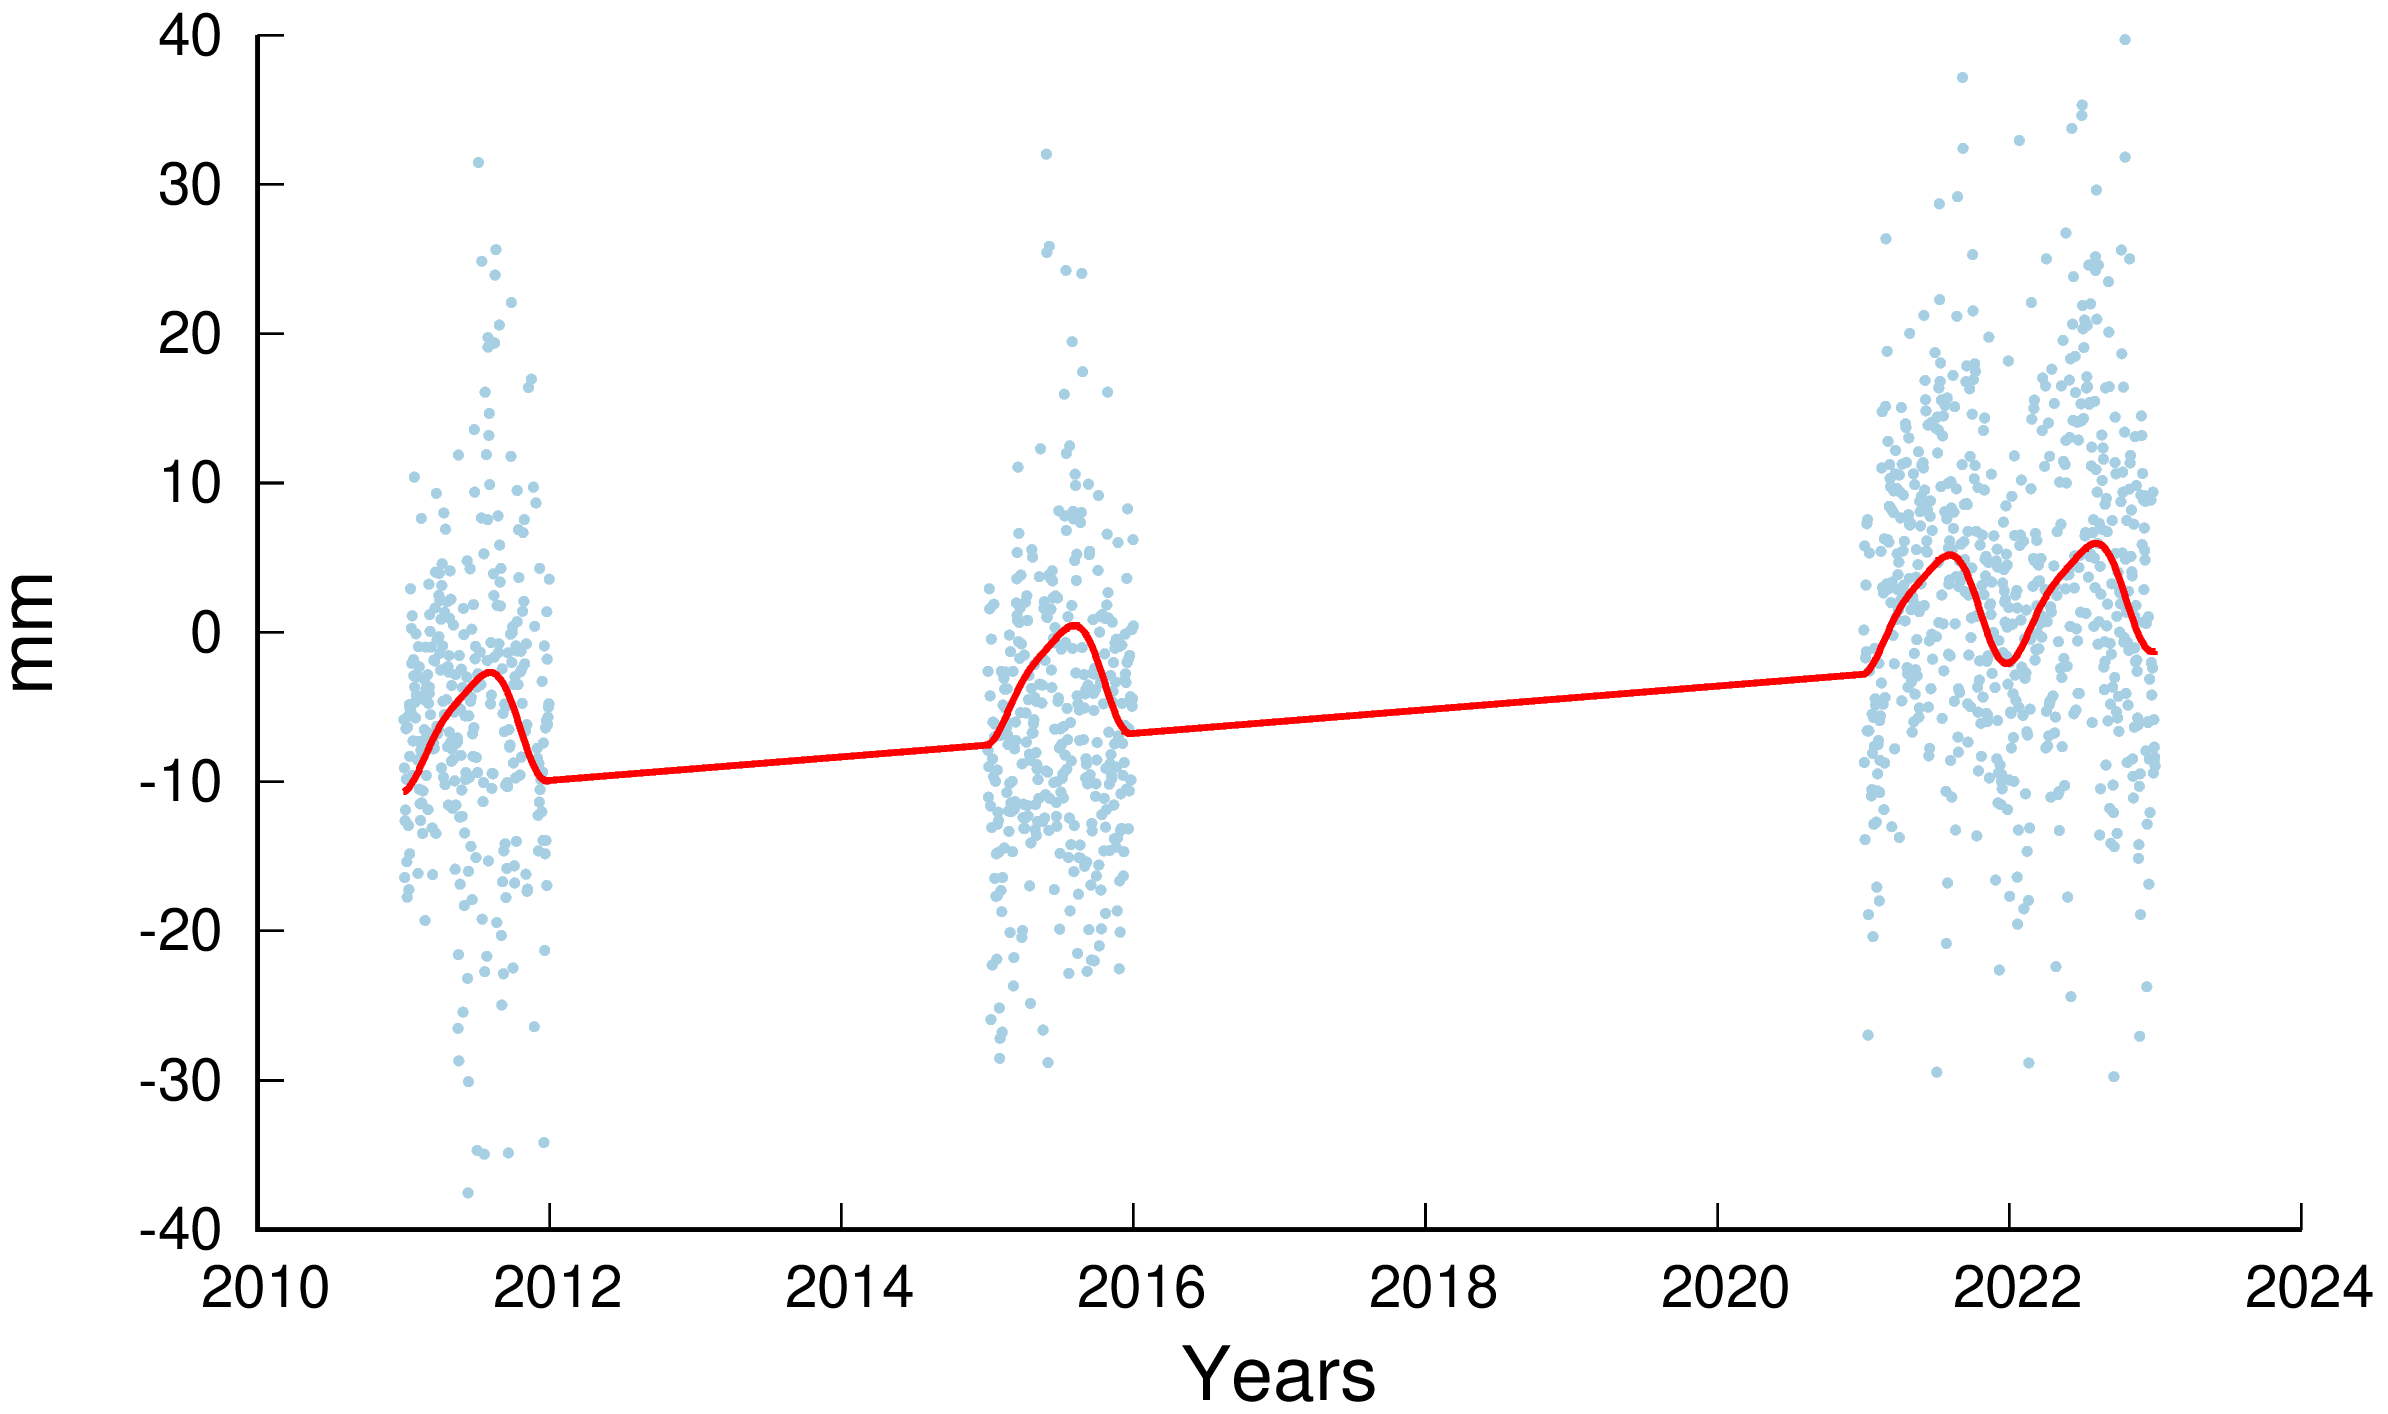
\includegraphics[width=.75\textwidth]{098a_2_data.png}
       \end{center} 
    \end{column}
    \begin{column}{.33\textwidth}
      \begin{center}
      Station:\textbf{057A}\\
         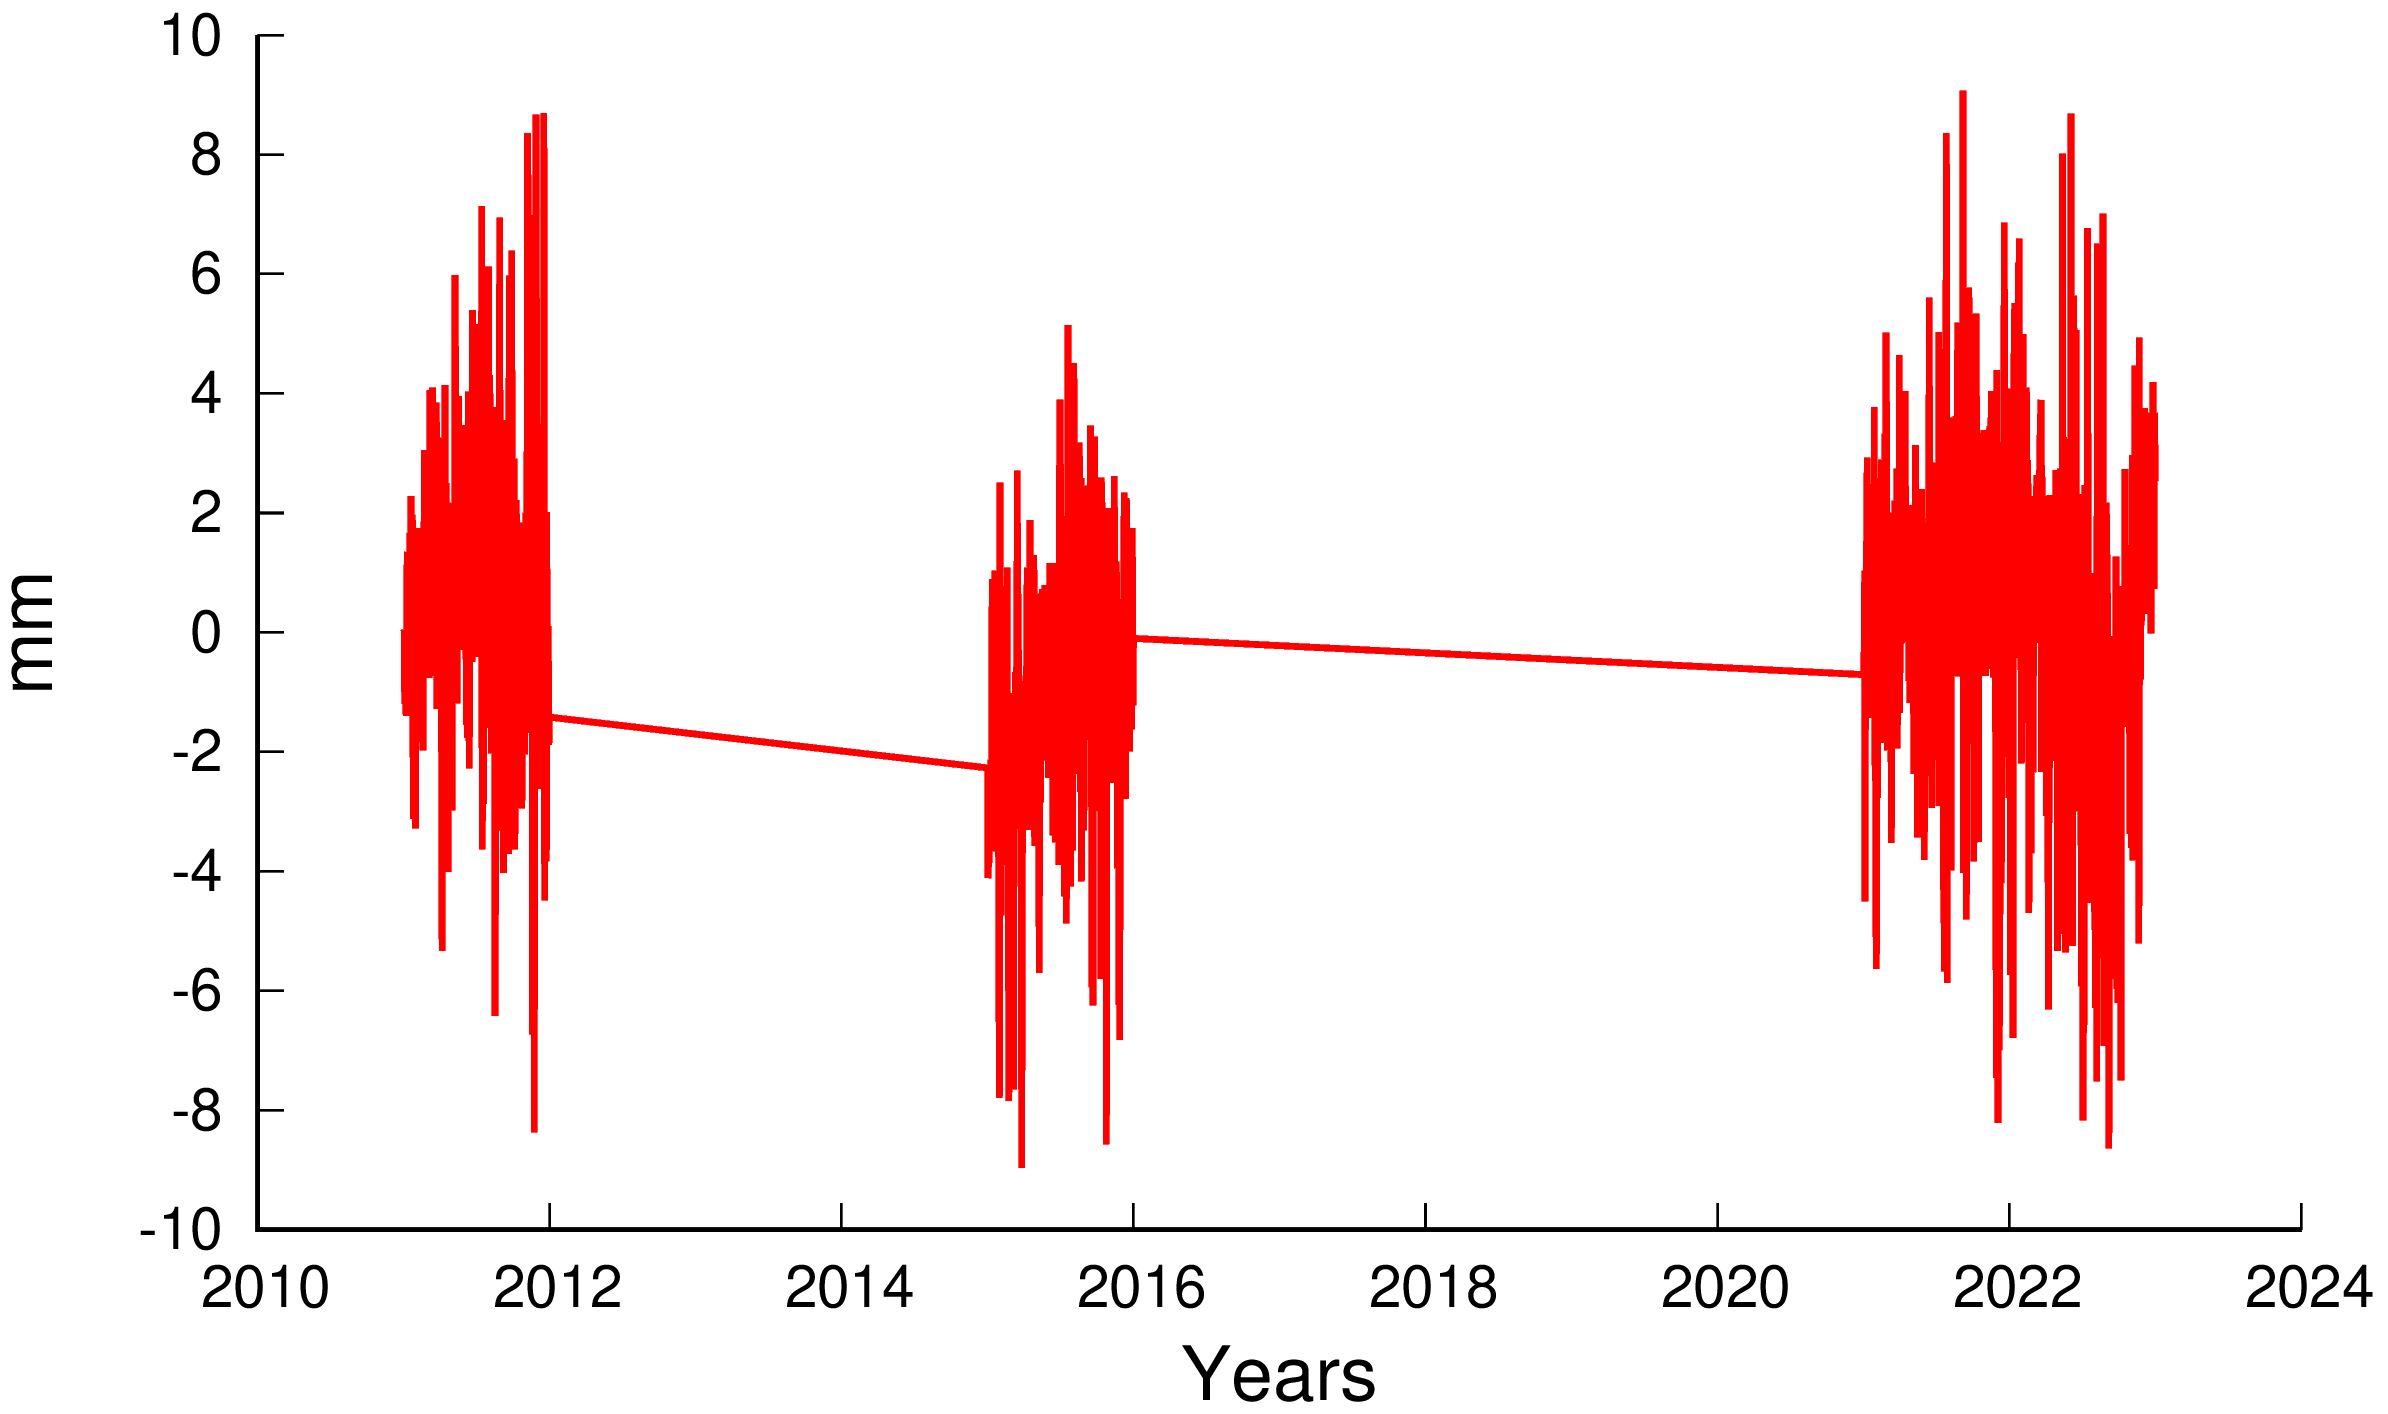
\includegraphics[width=.75\textwidth]{098a_0_res.png}\\
         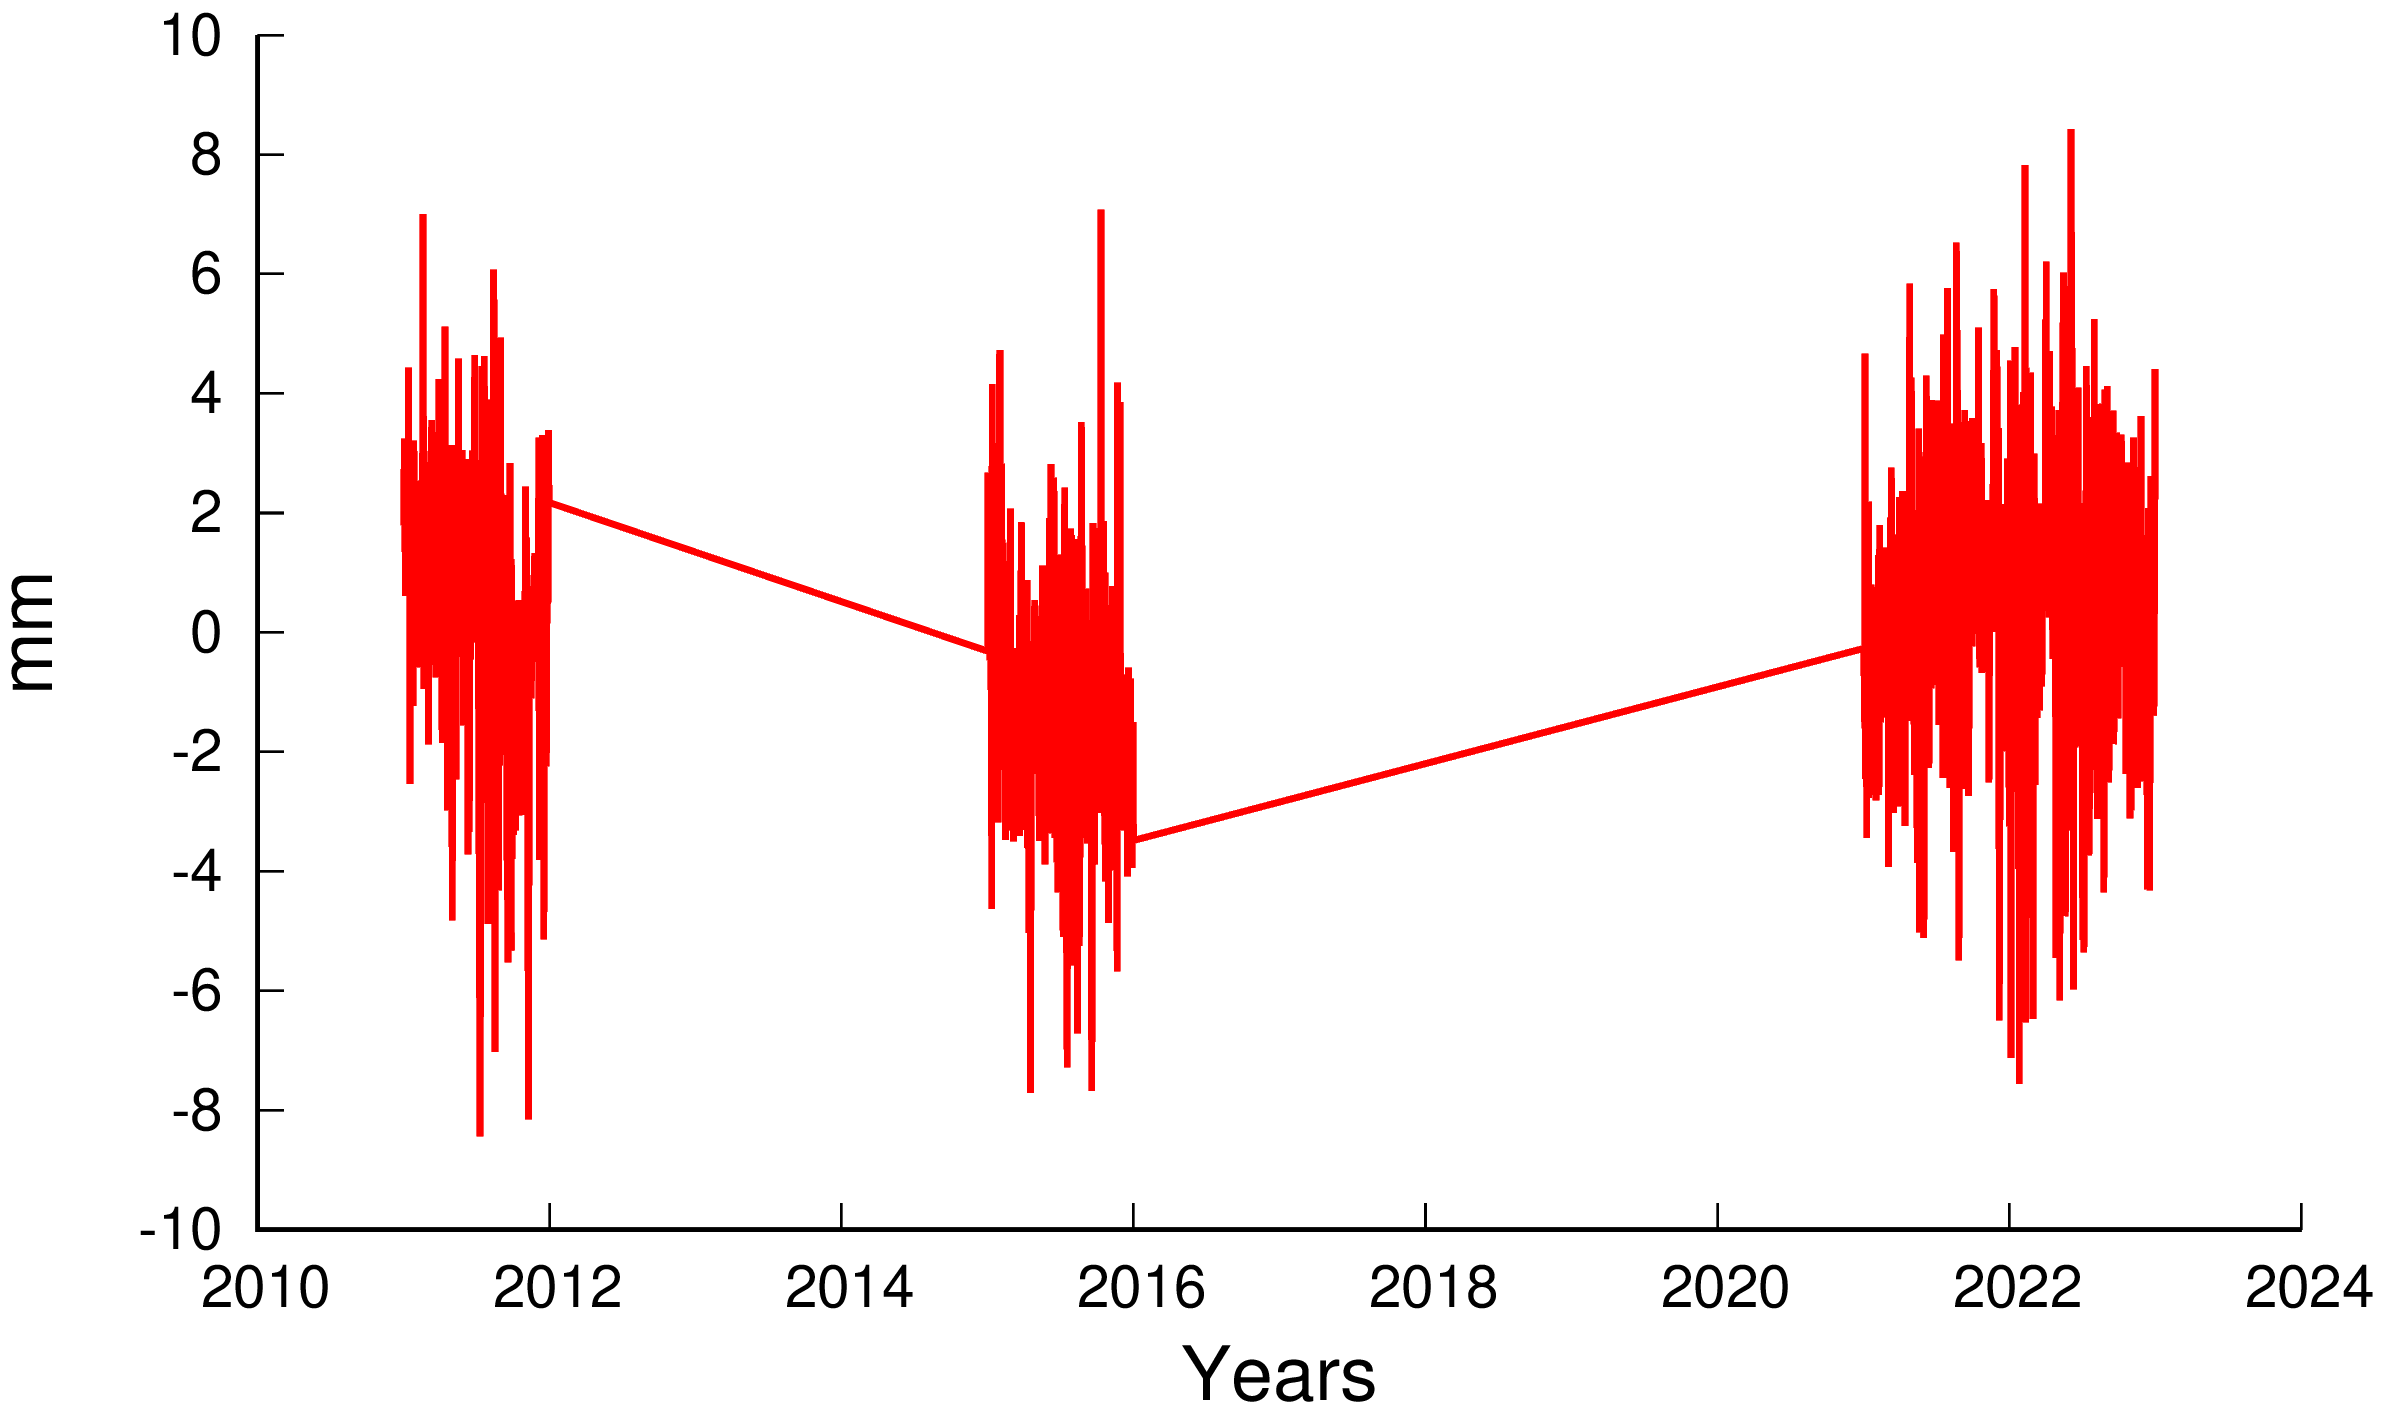
\includegraphics[width=.75\textwidth]{098a_1_res.png}\\
         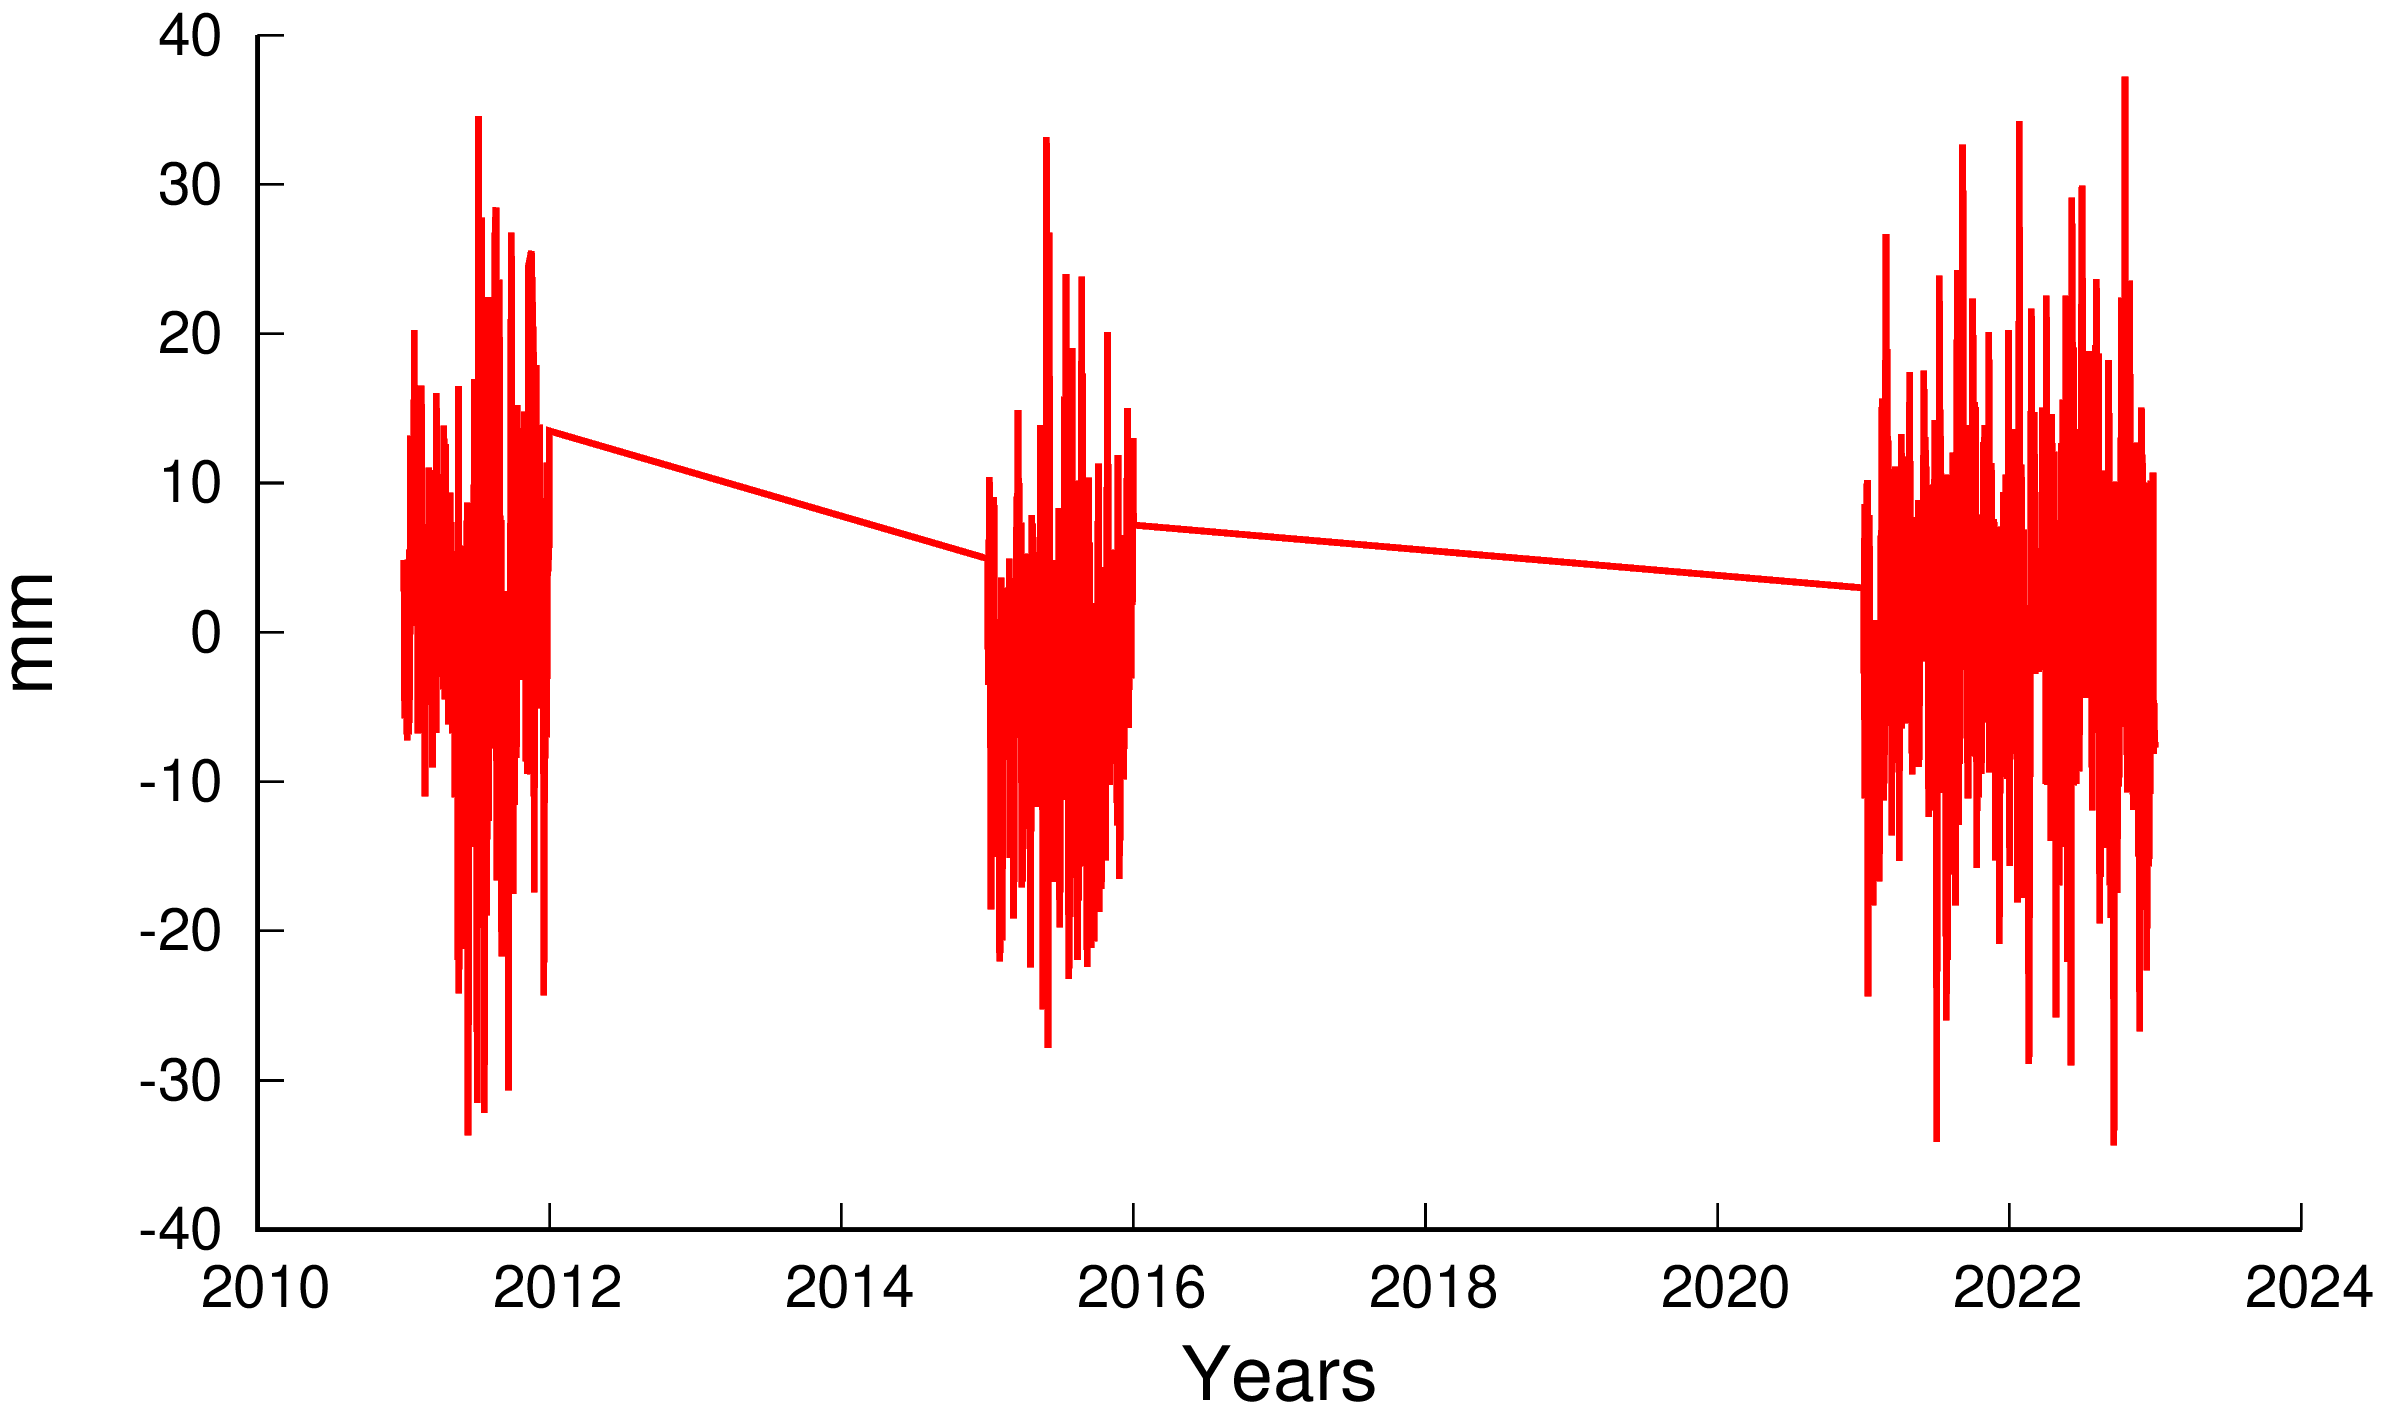
\includegraphics[width=.75\textwidth]{098a_2_res.png}
       \end{center} 
    \end{column}
  \end{columns}
\end{frame}
\note{}

 % ------------------------------------------------------------------------------
\begin{frame}
  \frametitle{Ειδικές περιπτώσεις - Σαντορίνη}
  \framesubtitle{}
  \label{}
  \vskip-1cm
  \begin{columns}[T]
    \begin{column}{.33\textwidth}
    \vskip.5cm
    Εκτίμηση αλλαγή ταχυτήτων στον σταθμό της Σαντορίνης:
%    \begin{table}[H]{\small
%    \begin{center}
%    \begin{tabular*}{.97\linewidth}{@{\extracolsep{\fill}} l c c}
%      \toprule
%        comp & < $\sim$2013 & > $\sim$ 2013\\
%             & \multicolumn{2}{c}{(mm/yr)}\\
%      \midrule
%        north & -30.1 & -17.5 \\
%        east  &  31.3 & 7.0 \\
%        up    &  17.2 & 2.1 \\
%      \bottomrule
%    \end{tabular*}
%    \end{center}}
%    \end{table}


    \end{column}
    \begin{column}{.33\textwidth}
      \begin{center}
      Station:\textbf{048A}\\
         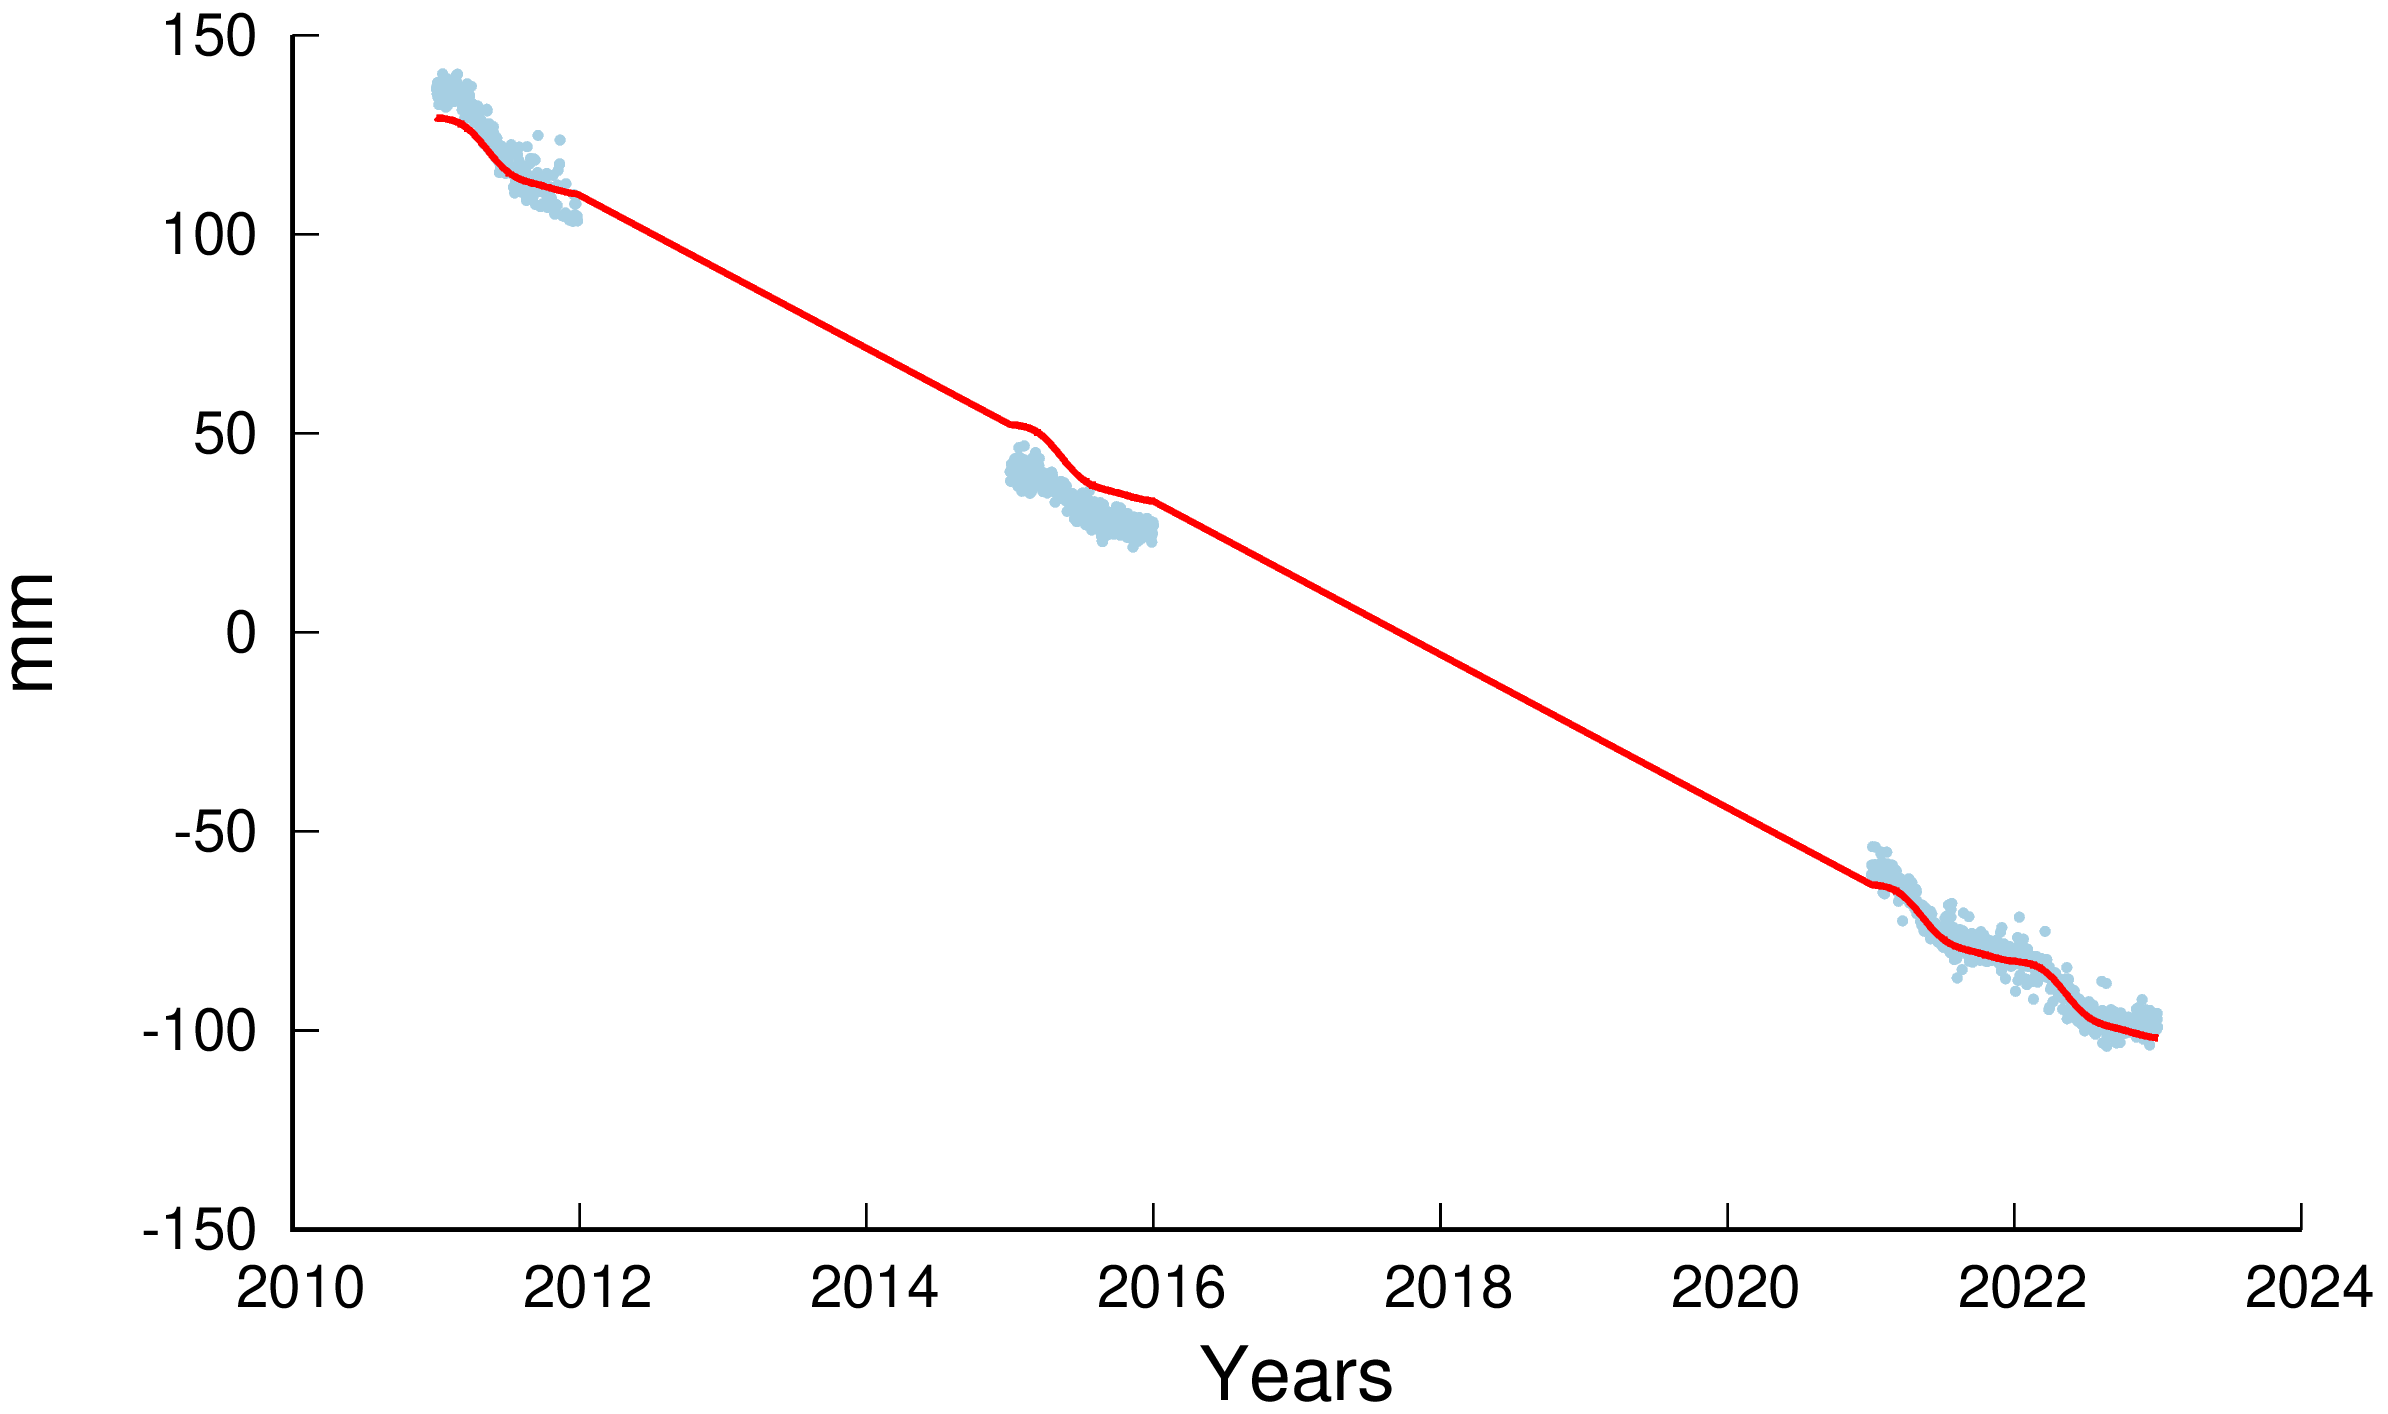
\includegraphics[width=.75\textwidth]{048a_0_data_nomod.png}\\
         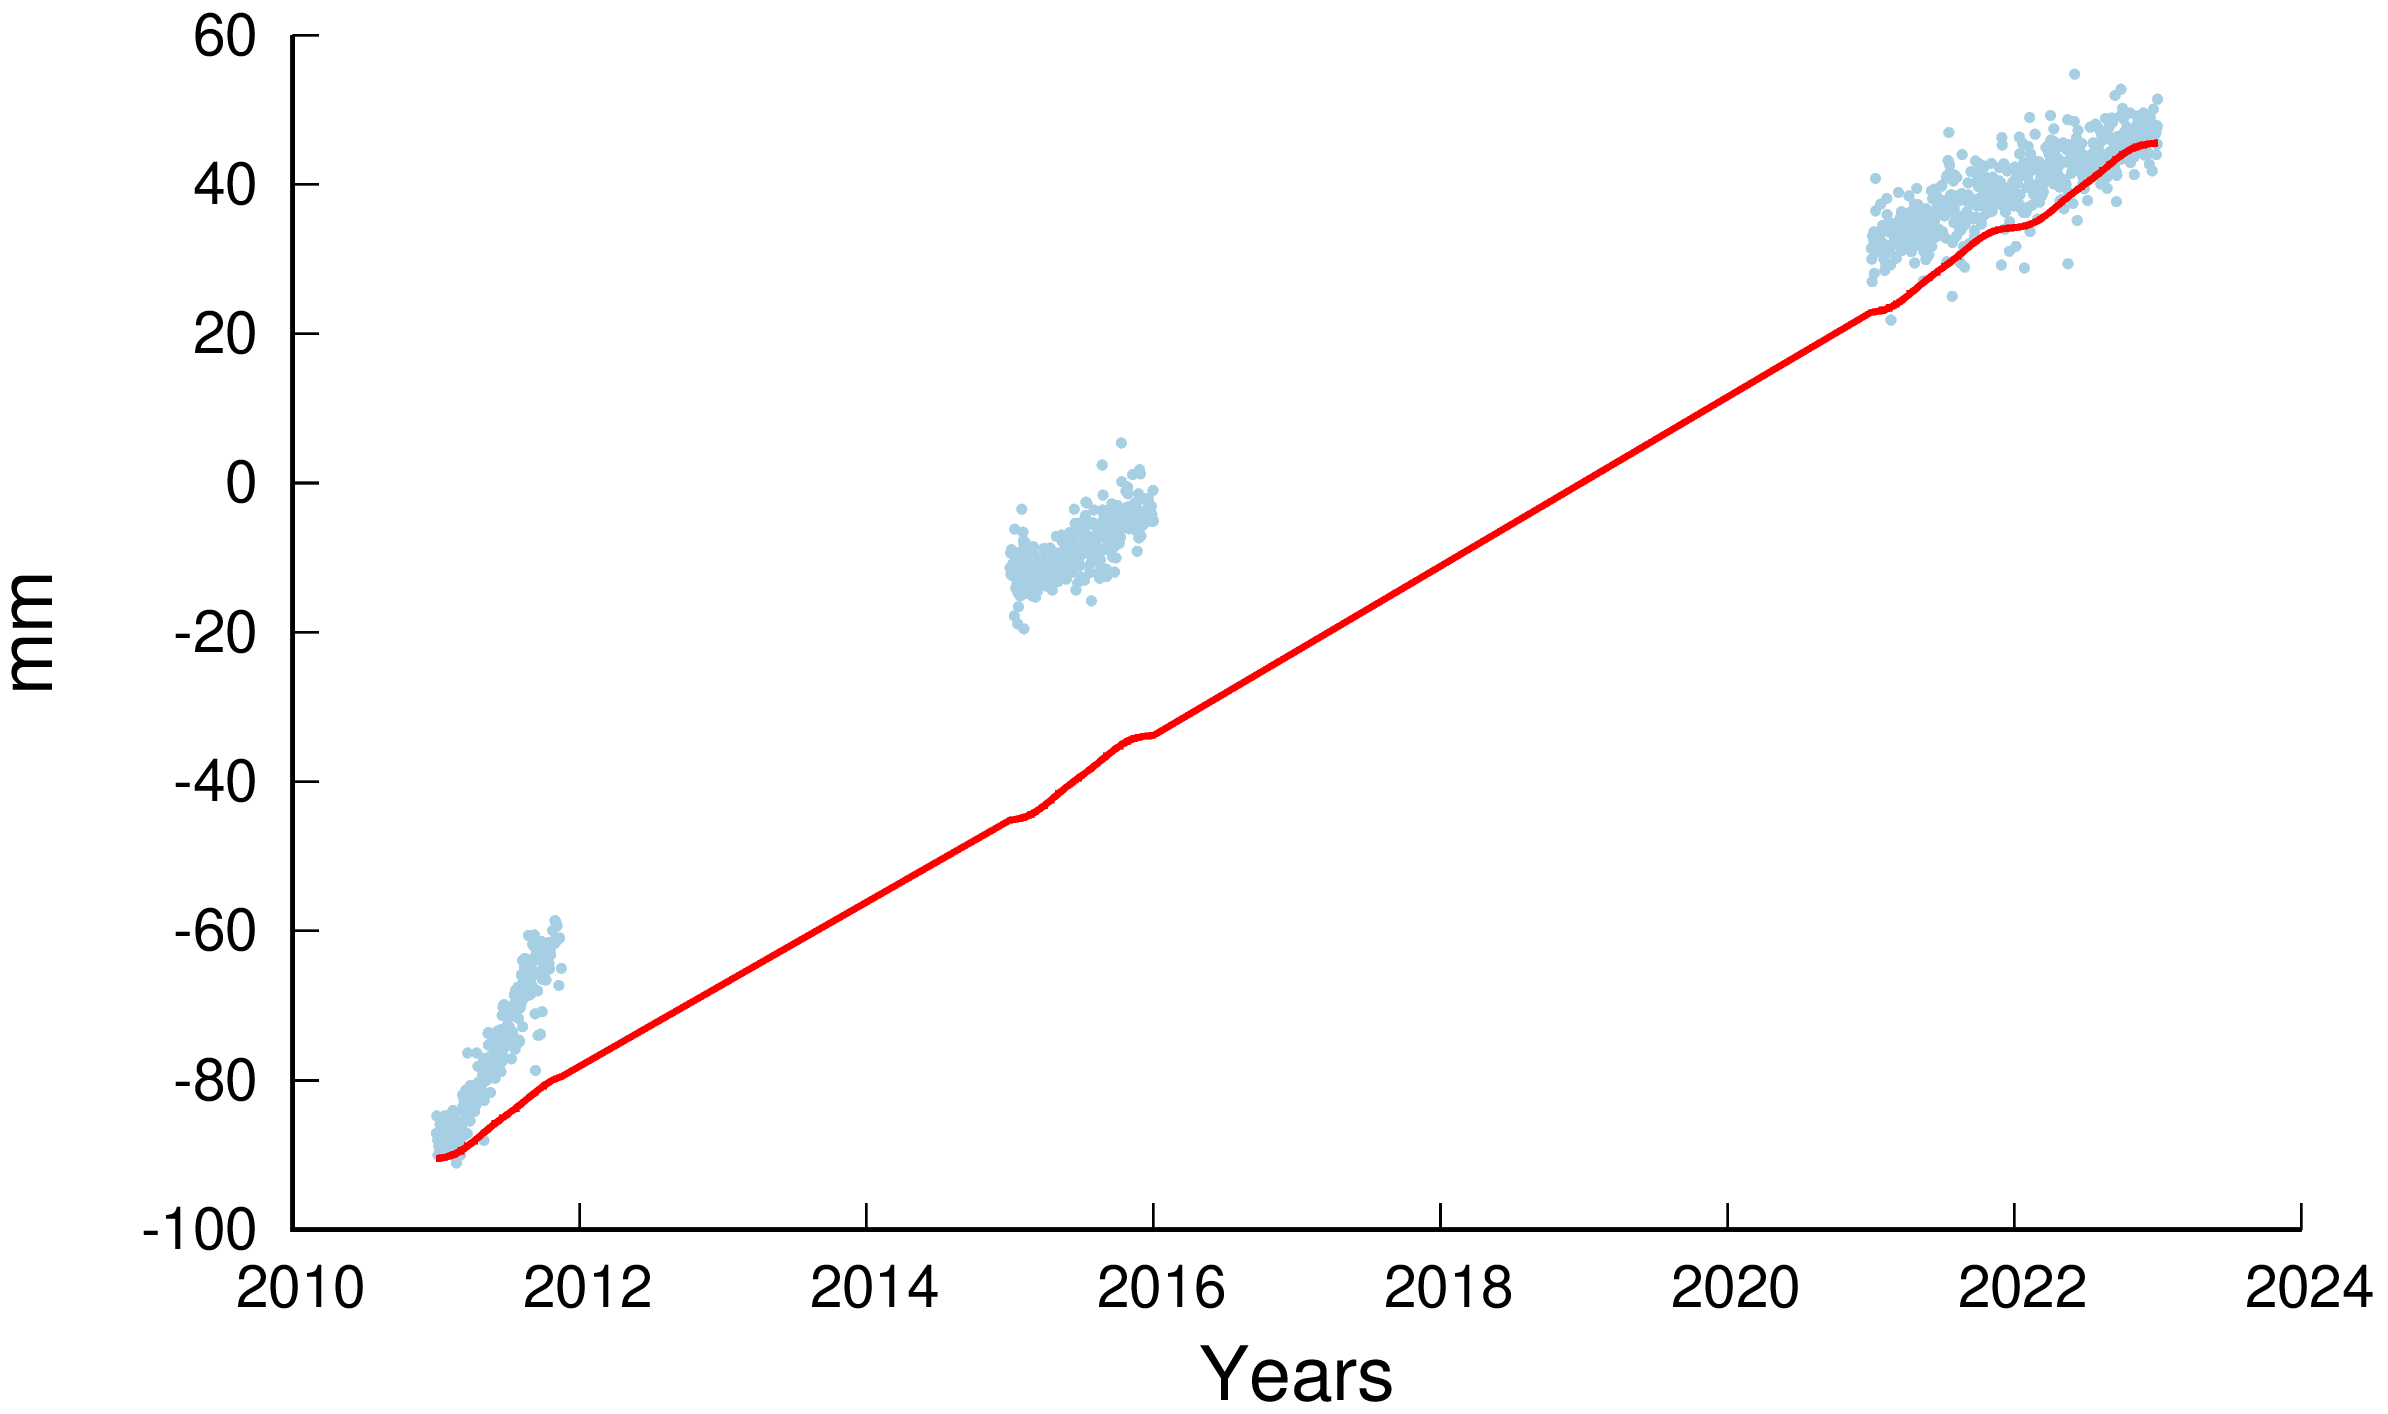
\includegraphics[width=.75\textwidth]{048a_1_data_nomod.png}\\
         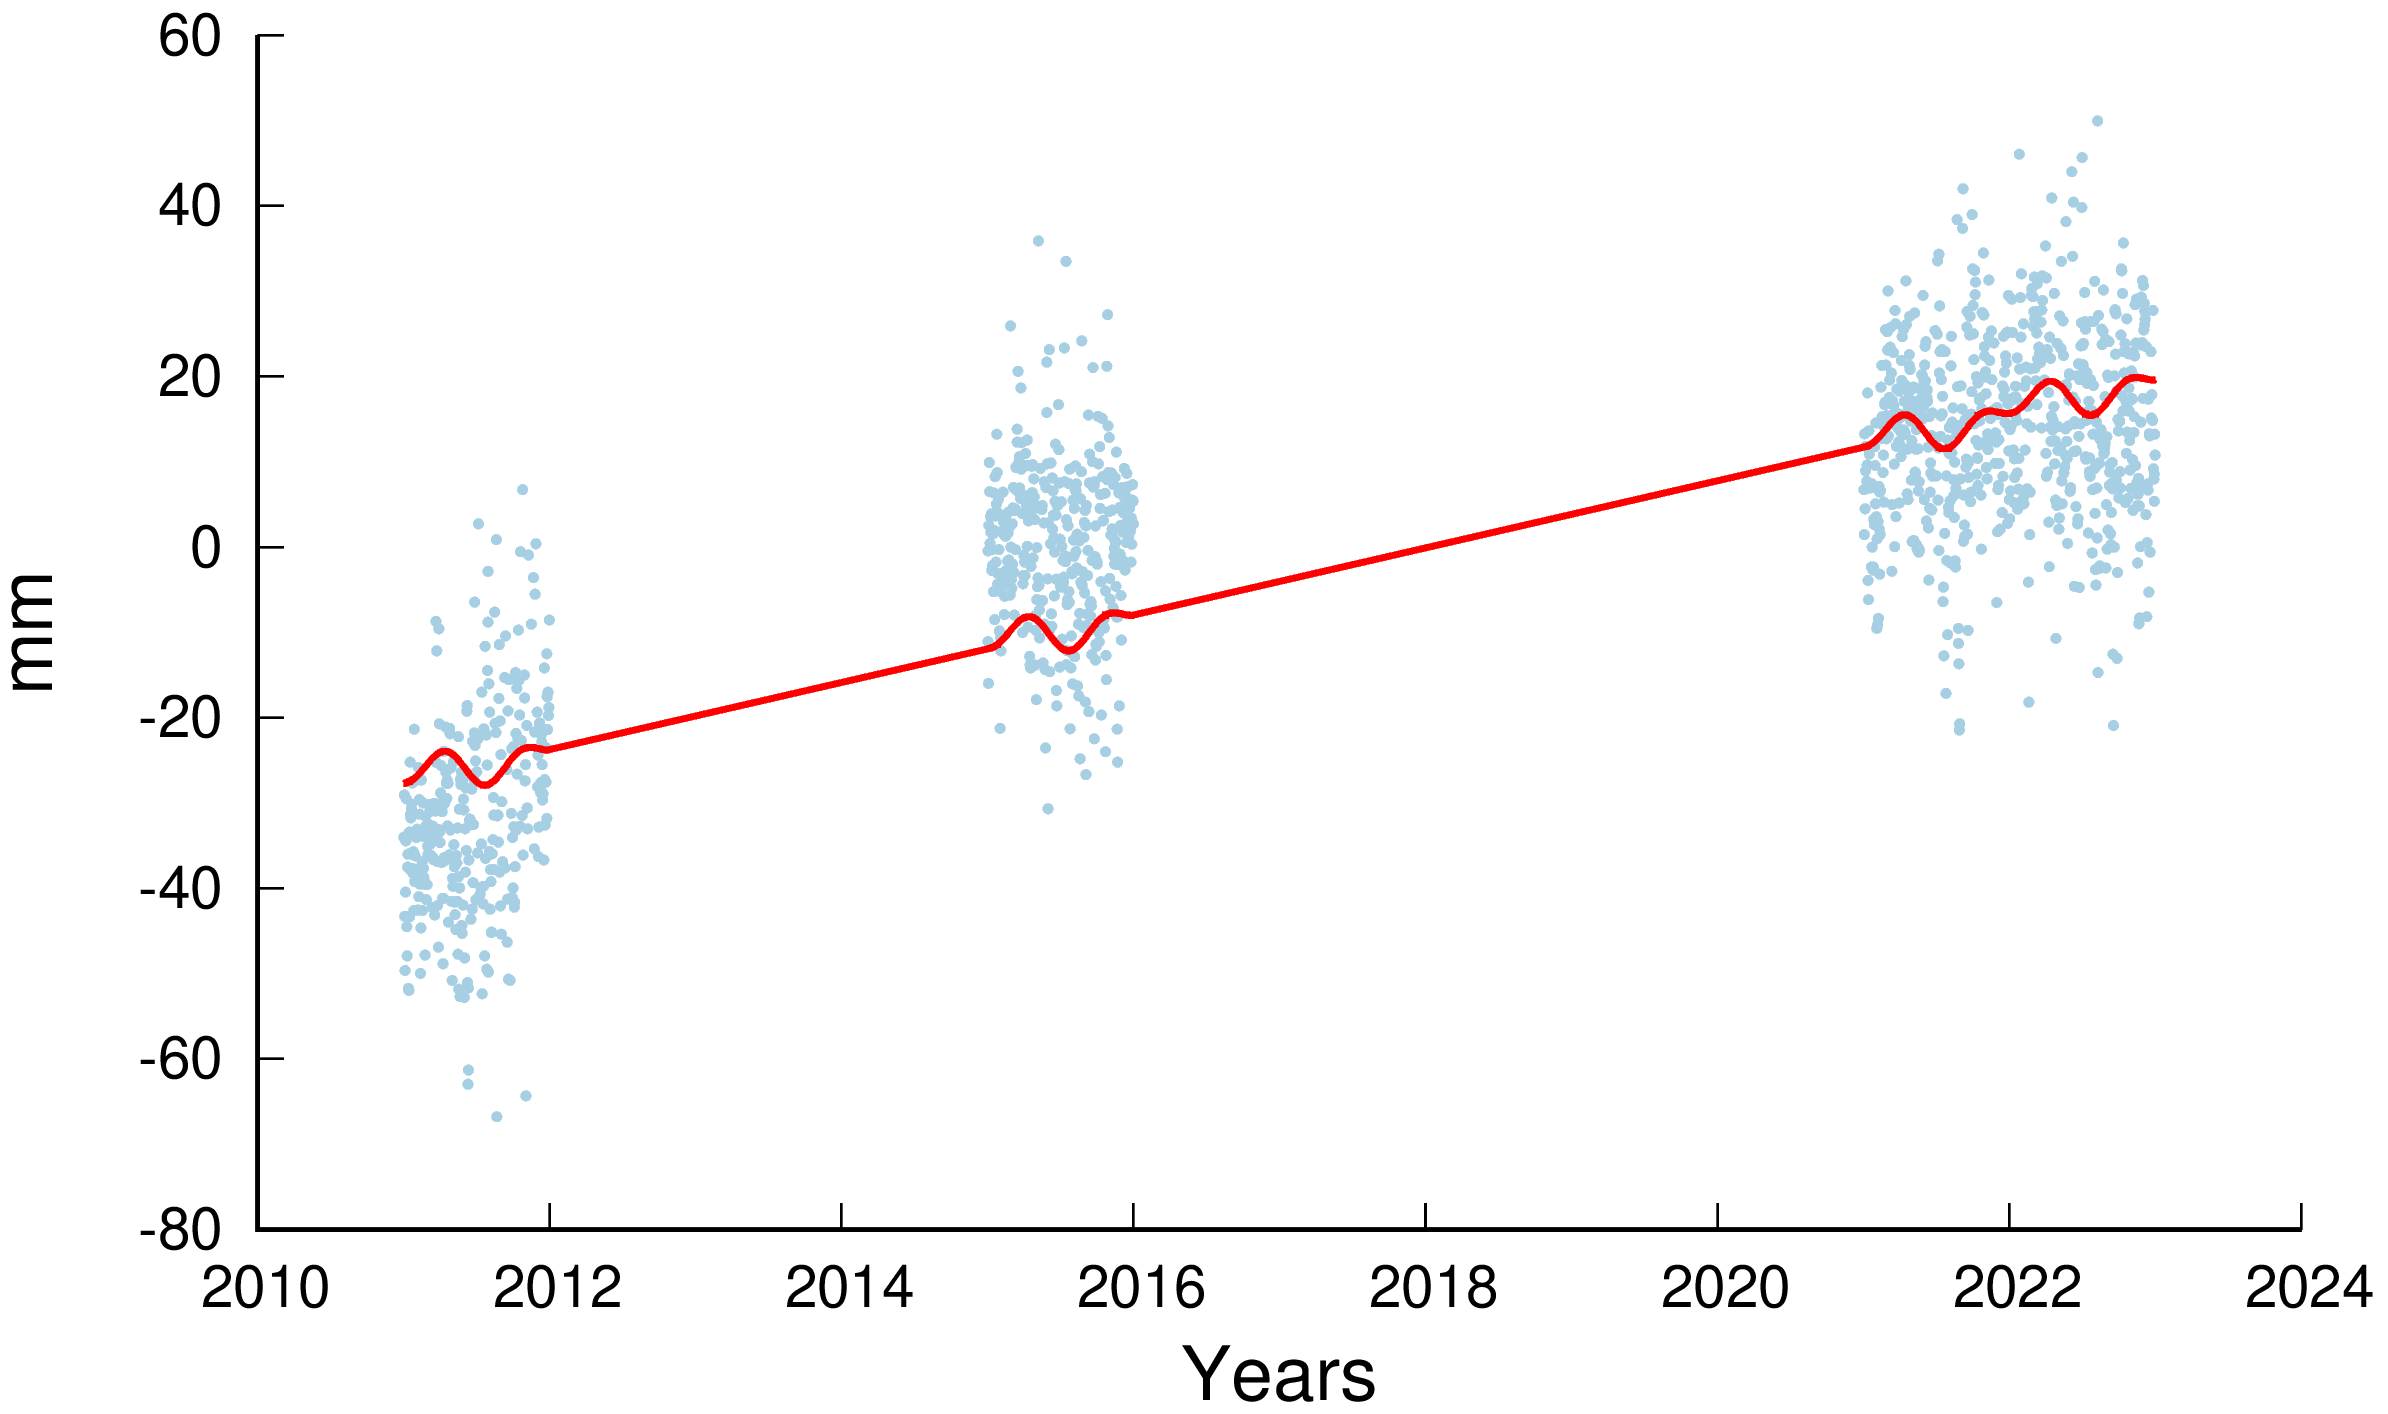
\includegraphics[width=.75\textwidth]{048a_2_data_nomod.png}
       \end{center} 
    \end{column}
    \begin{column}{.33\textwidth}
      \begin{center}
      Residuals:\textbf{048A}\\
         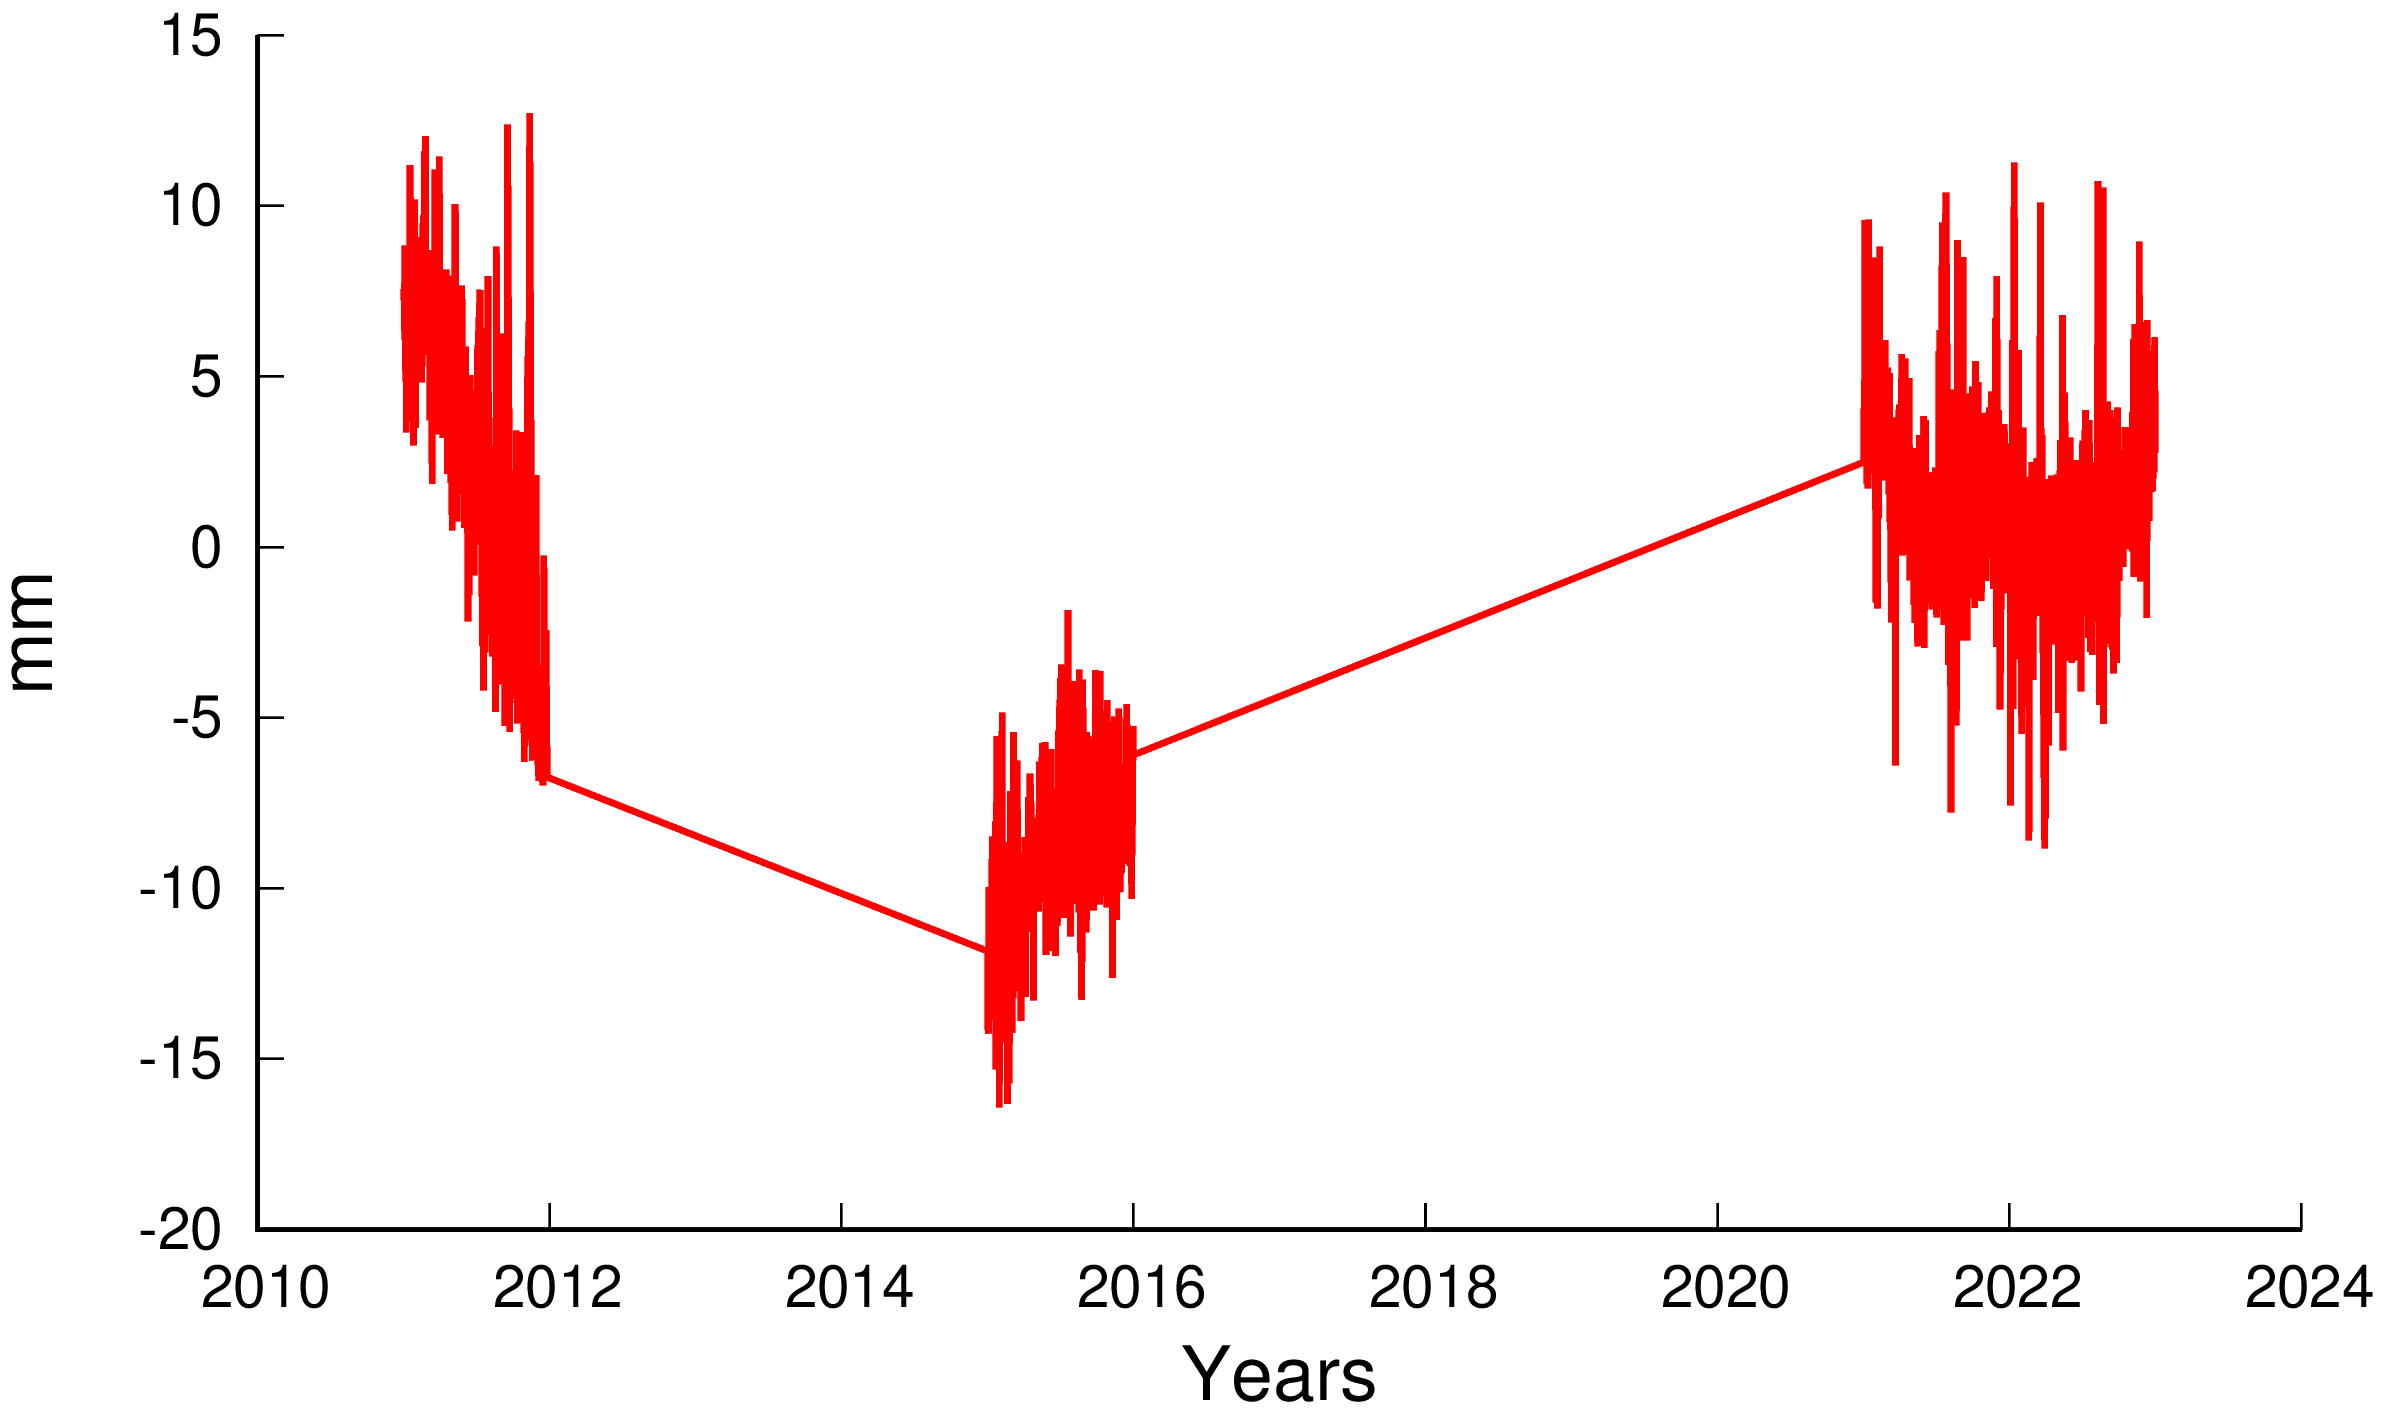
\includegraphics[width=.75\textwidth]{048a_0_res_nomod.png}\\
         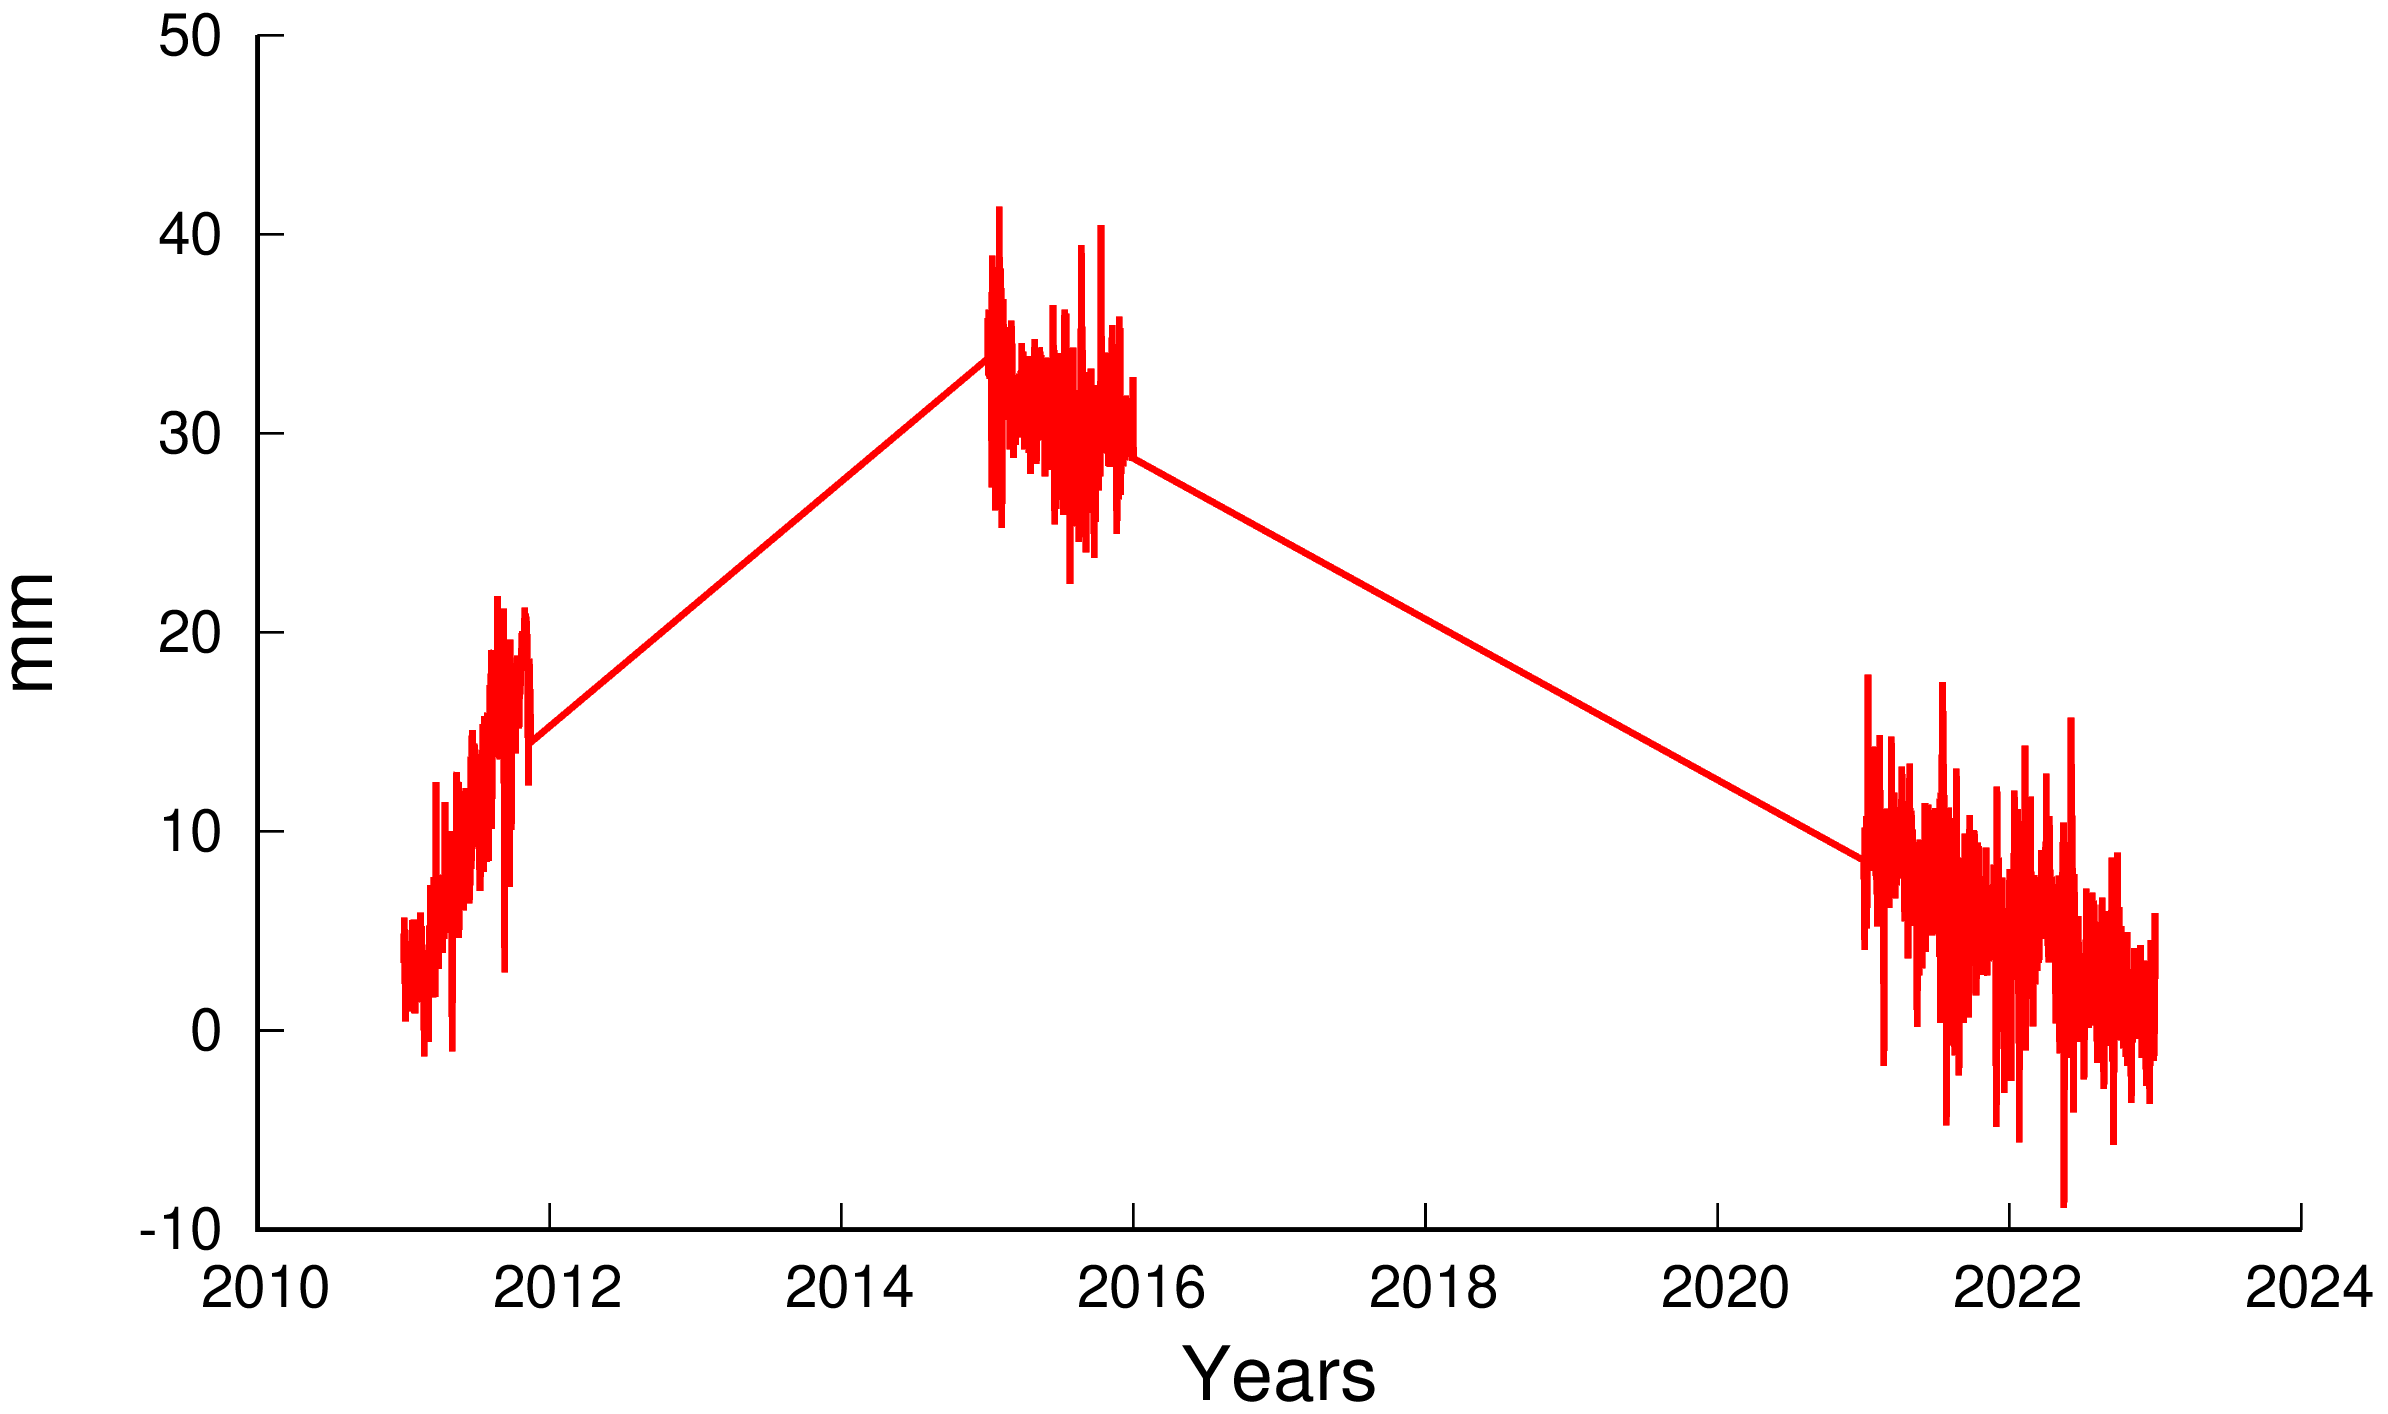
\includegraphics[width=.75\textwidth]{048a_1_res_nomod.png}\\
         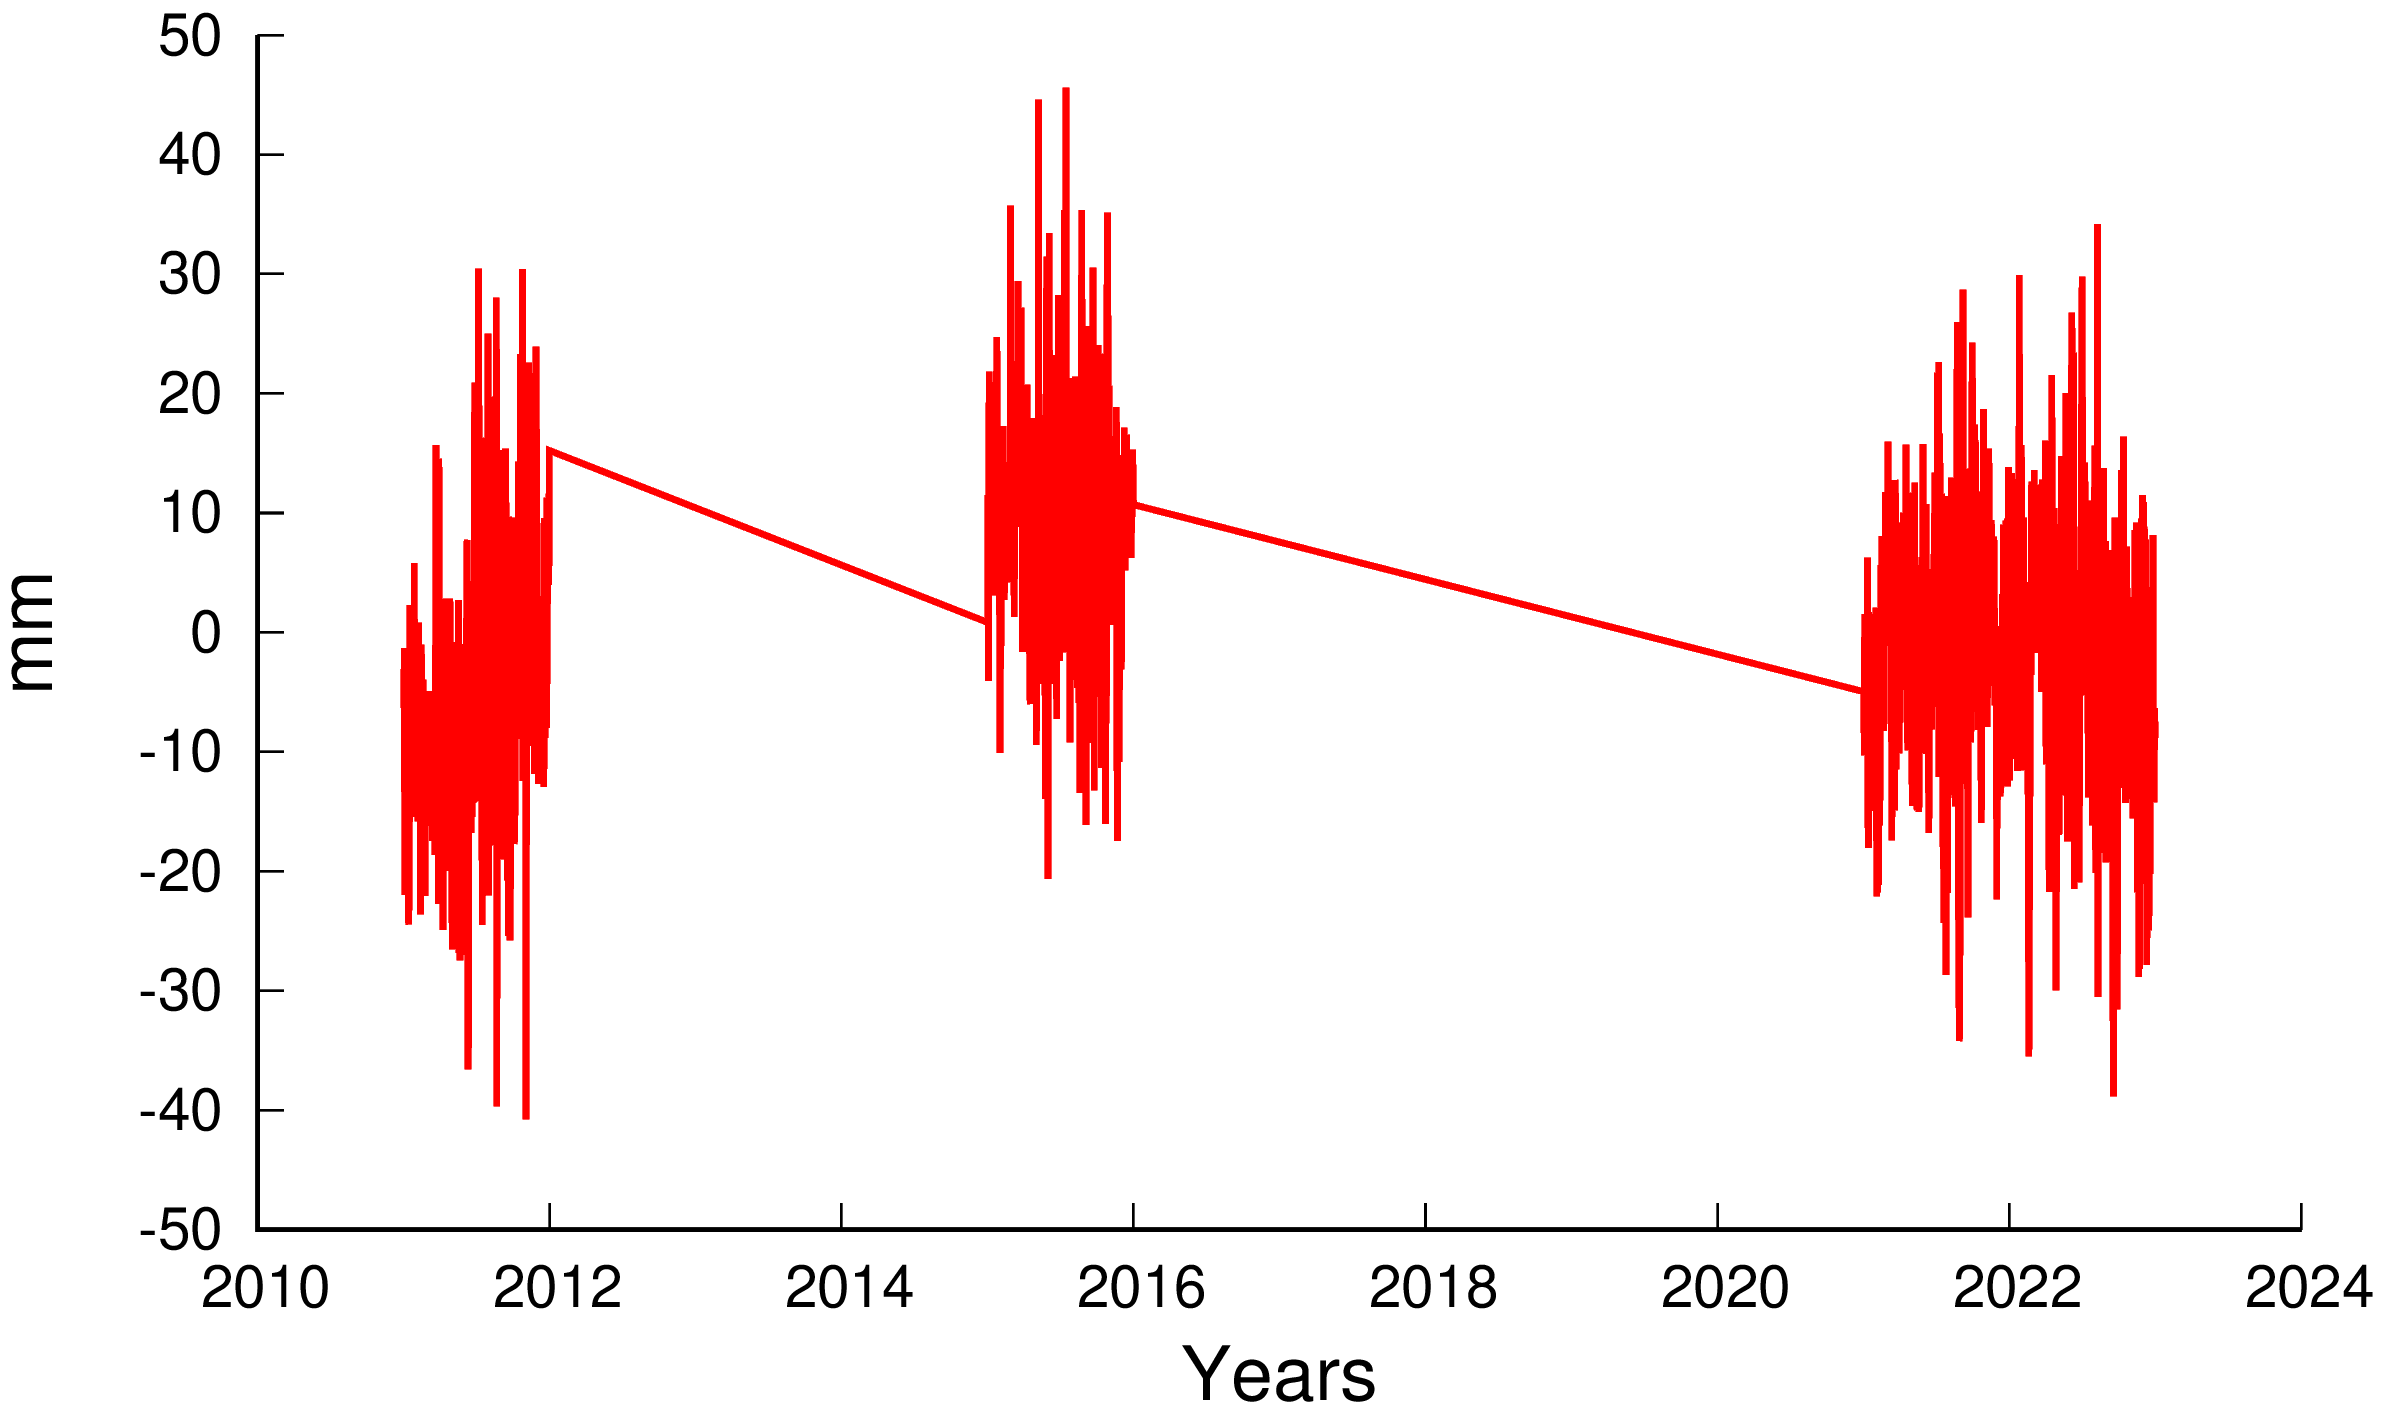
\includegraphics[width=.75\textwidth]{048a_2_res_nomod.png}
       \end{center} 
      
    \end{column}
  \end{columns}
\end{frame}
\note{}

 % ------------------------------------------------------------------------------
\begin{frame}
  \frametitle{Ειδικές περιπτώσεις - Σαντορίνη}
  \framesubtitle{}
  \label{}
  \vskip-1cm
  \begin{columns}[T]
    \begin{column}{.33\textwidth}
    \vskip.5cm
    Εκτίμηση αλλαγή ταχυτήτων στον σταθμό της Σαντορίνης:
    \begin{table}[H]{\small
    \begin{center}
    \begin{tabular*}{.97\linewidth}{@{\extracolsep{\fill}} l c c}
      \toprule
        comp & < $\sim$2013 & > $\sim$ 2013\\
             & \multicolumn{2}{c}{(mm/yr)}\\
      \midrule
        north & -30.1 & -17.5 \\
        east  &  31.3 & 7.0 \\
        up    &  17.2 & 2.1 \\
      \bottomrule
    \end{tabular*}
    \end{center}}
    \end{table}


    \end{column}
    \begin{column}{.33\textwidth}
      \begin{center}
      Station:\textbf{048A}\\
         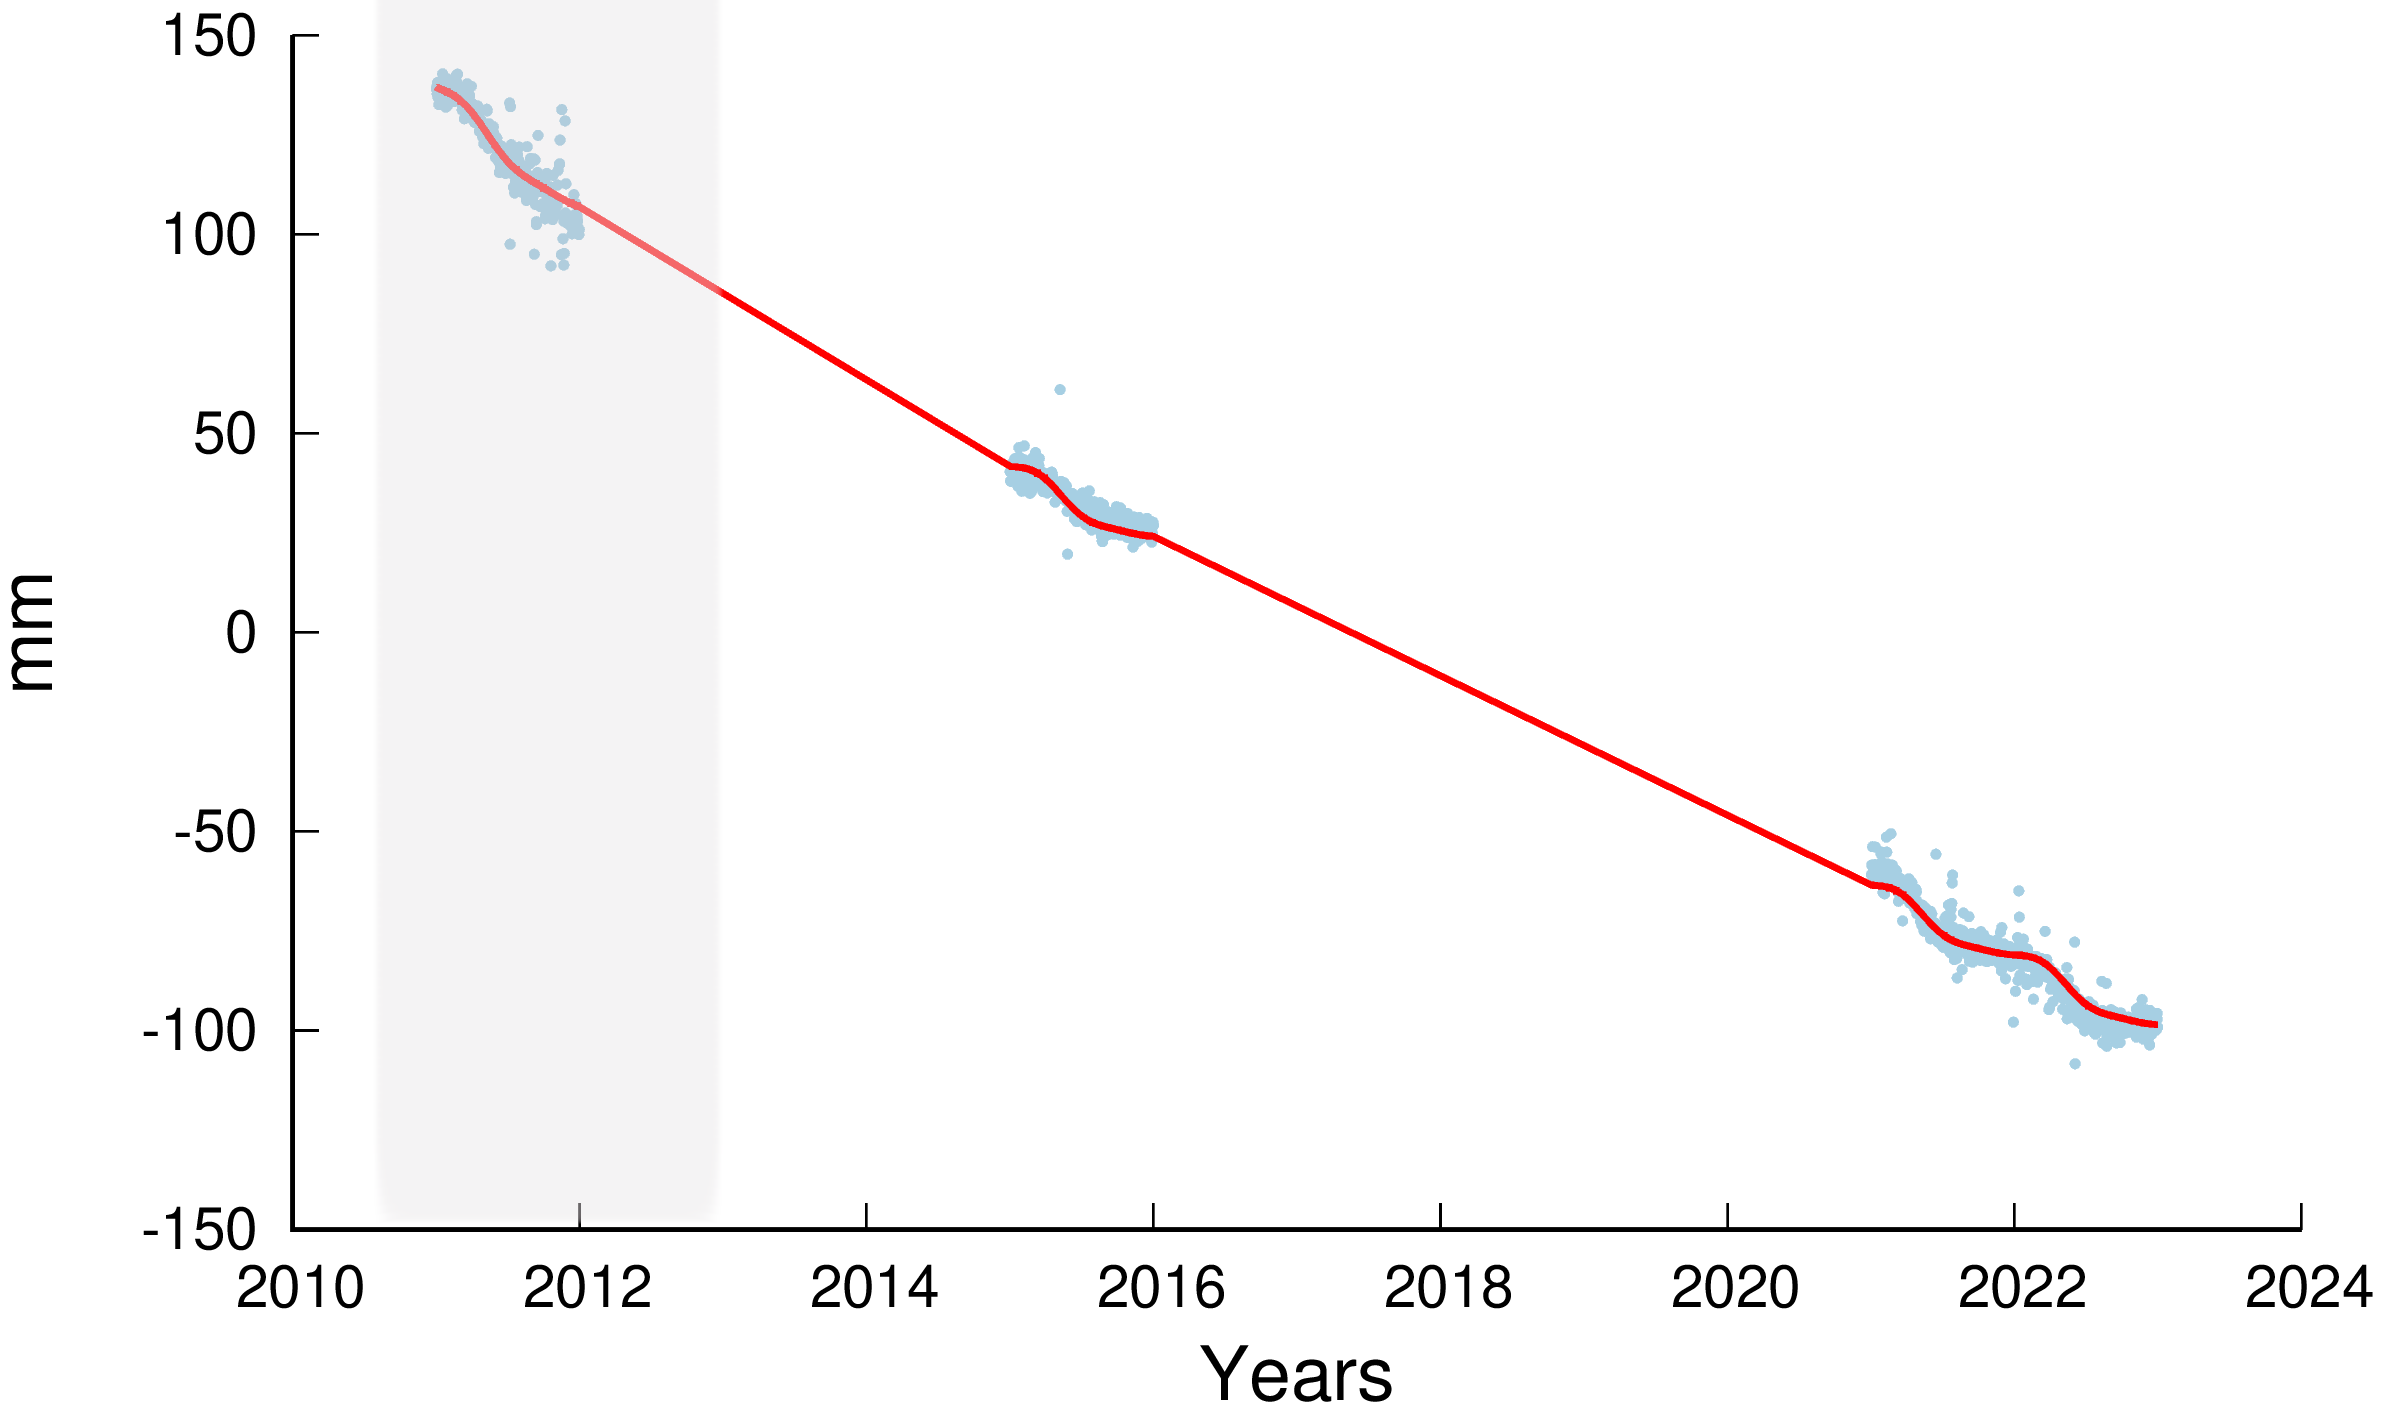
\includegraphics[width=.75\textwidth]{048a_0_data.png}\\
         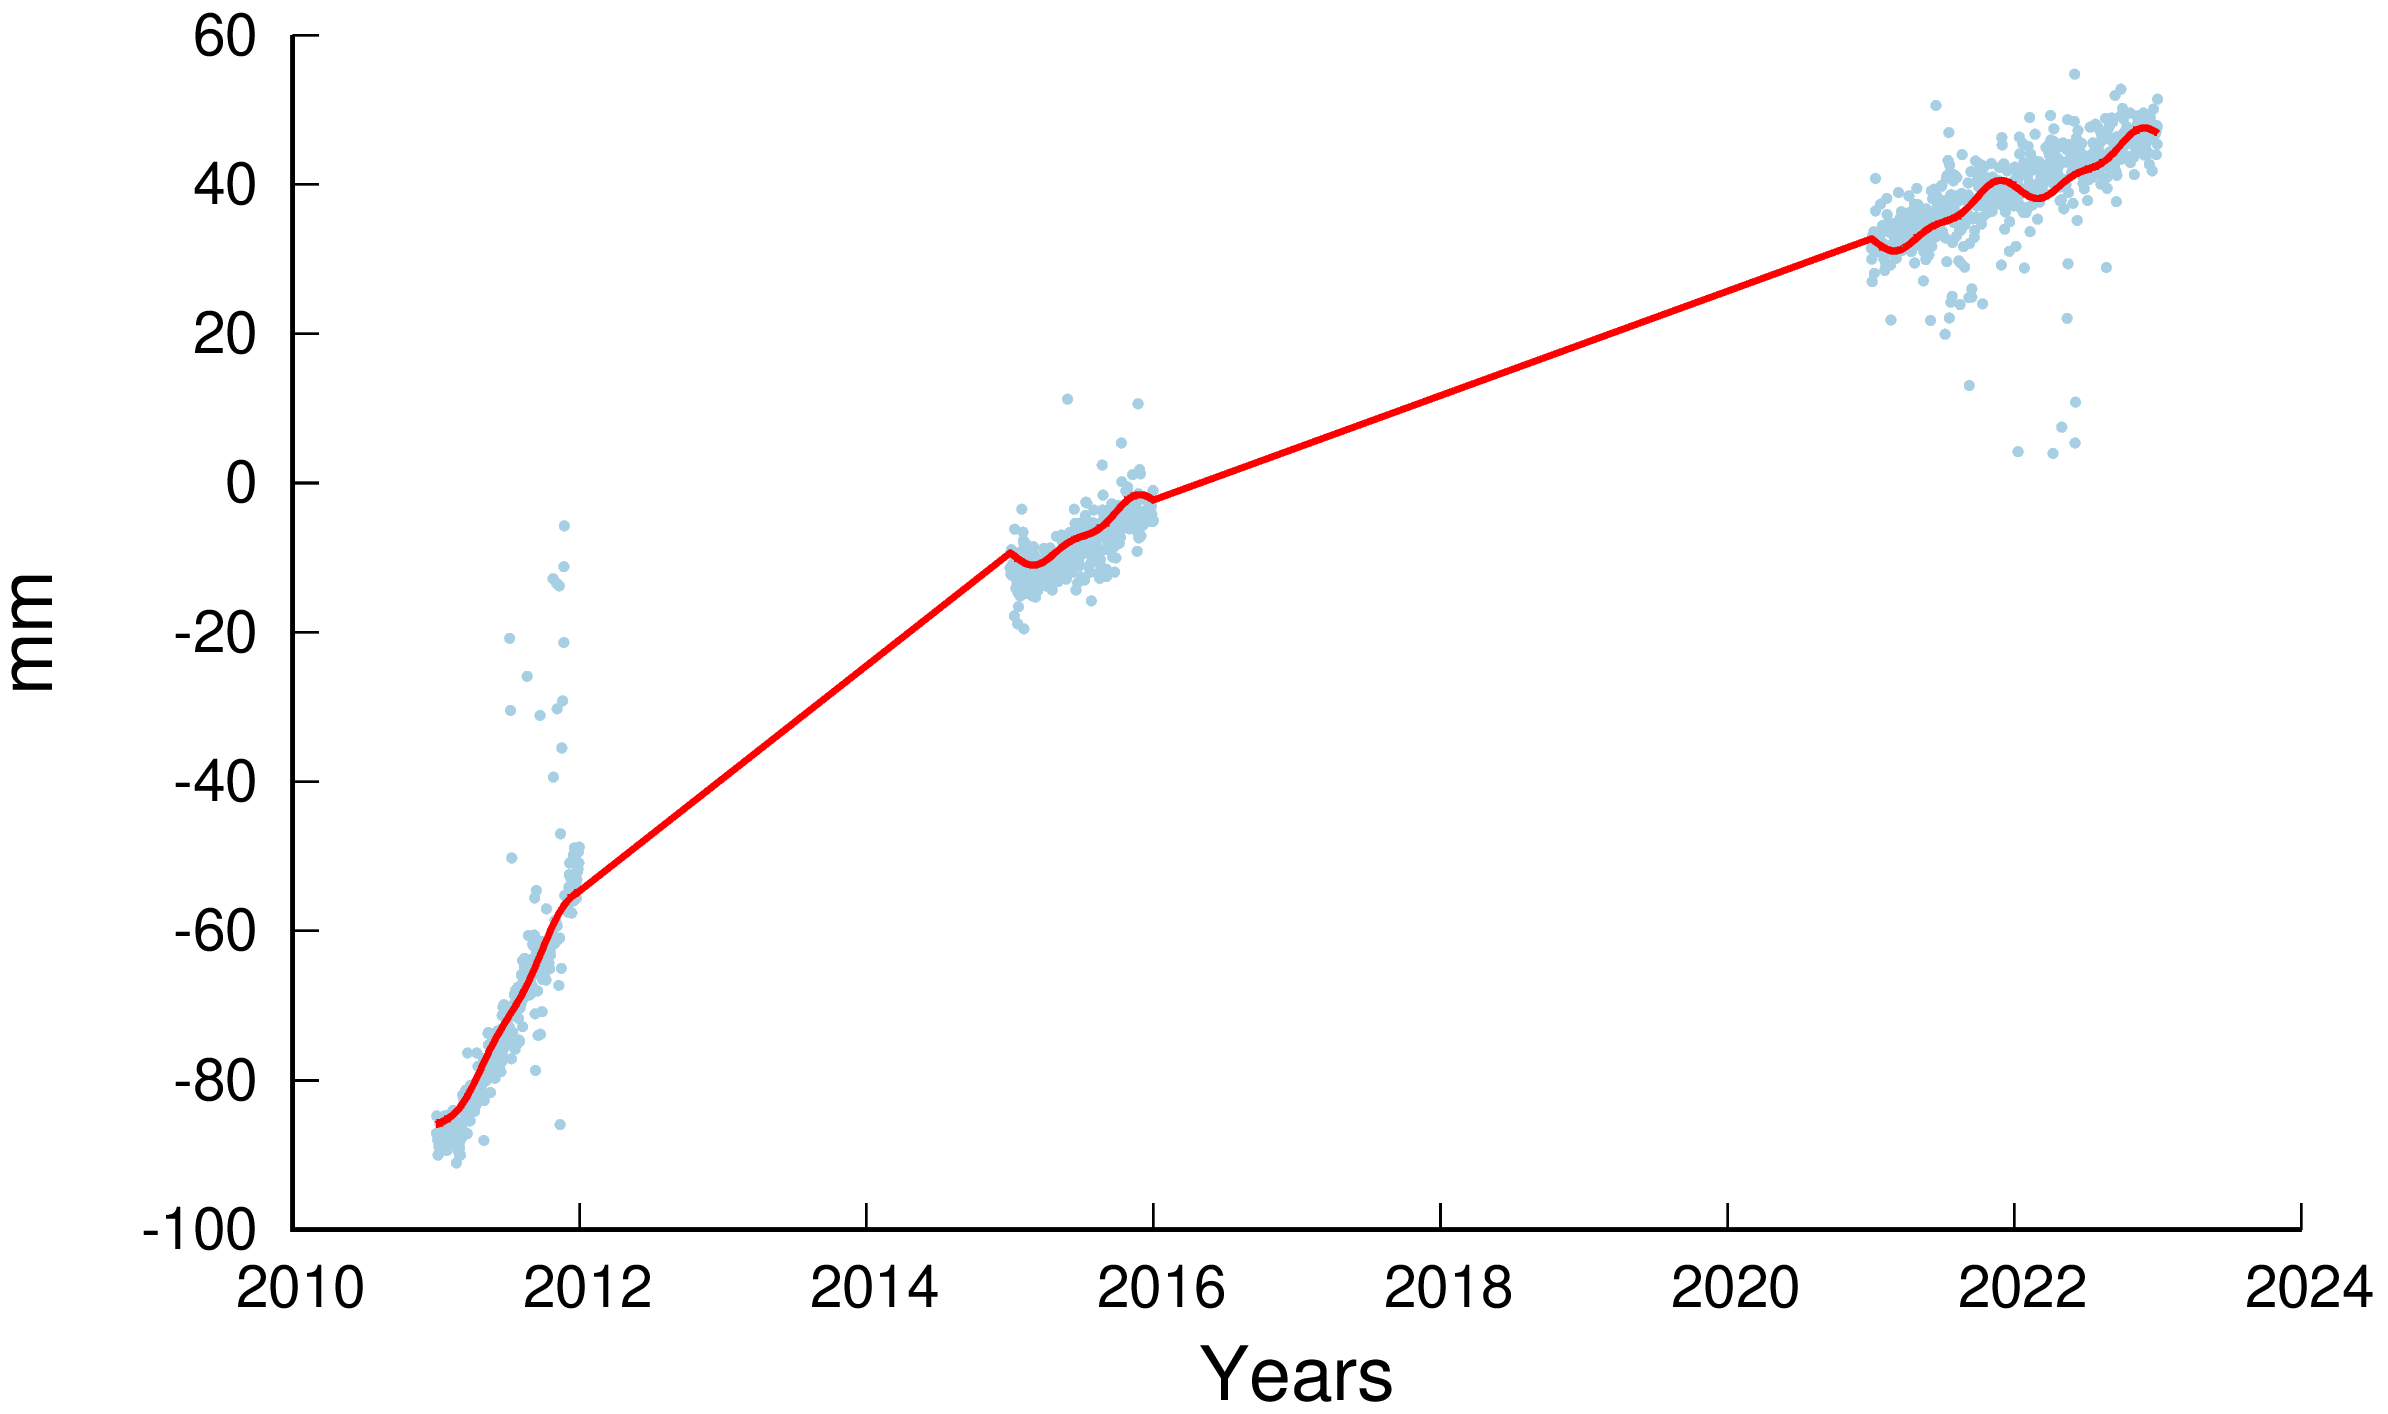
\includegraphics[width=.75\textwidth]{048a_1_data.png}\\
         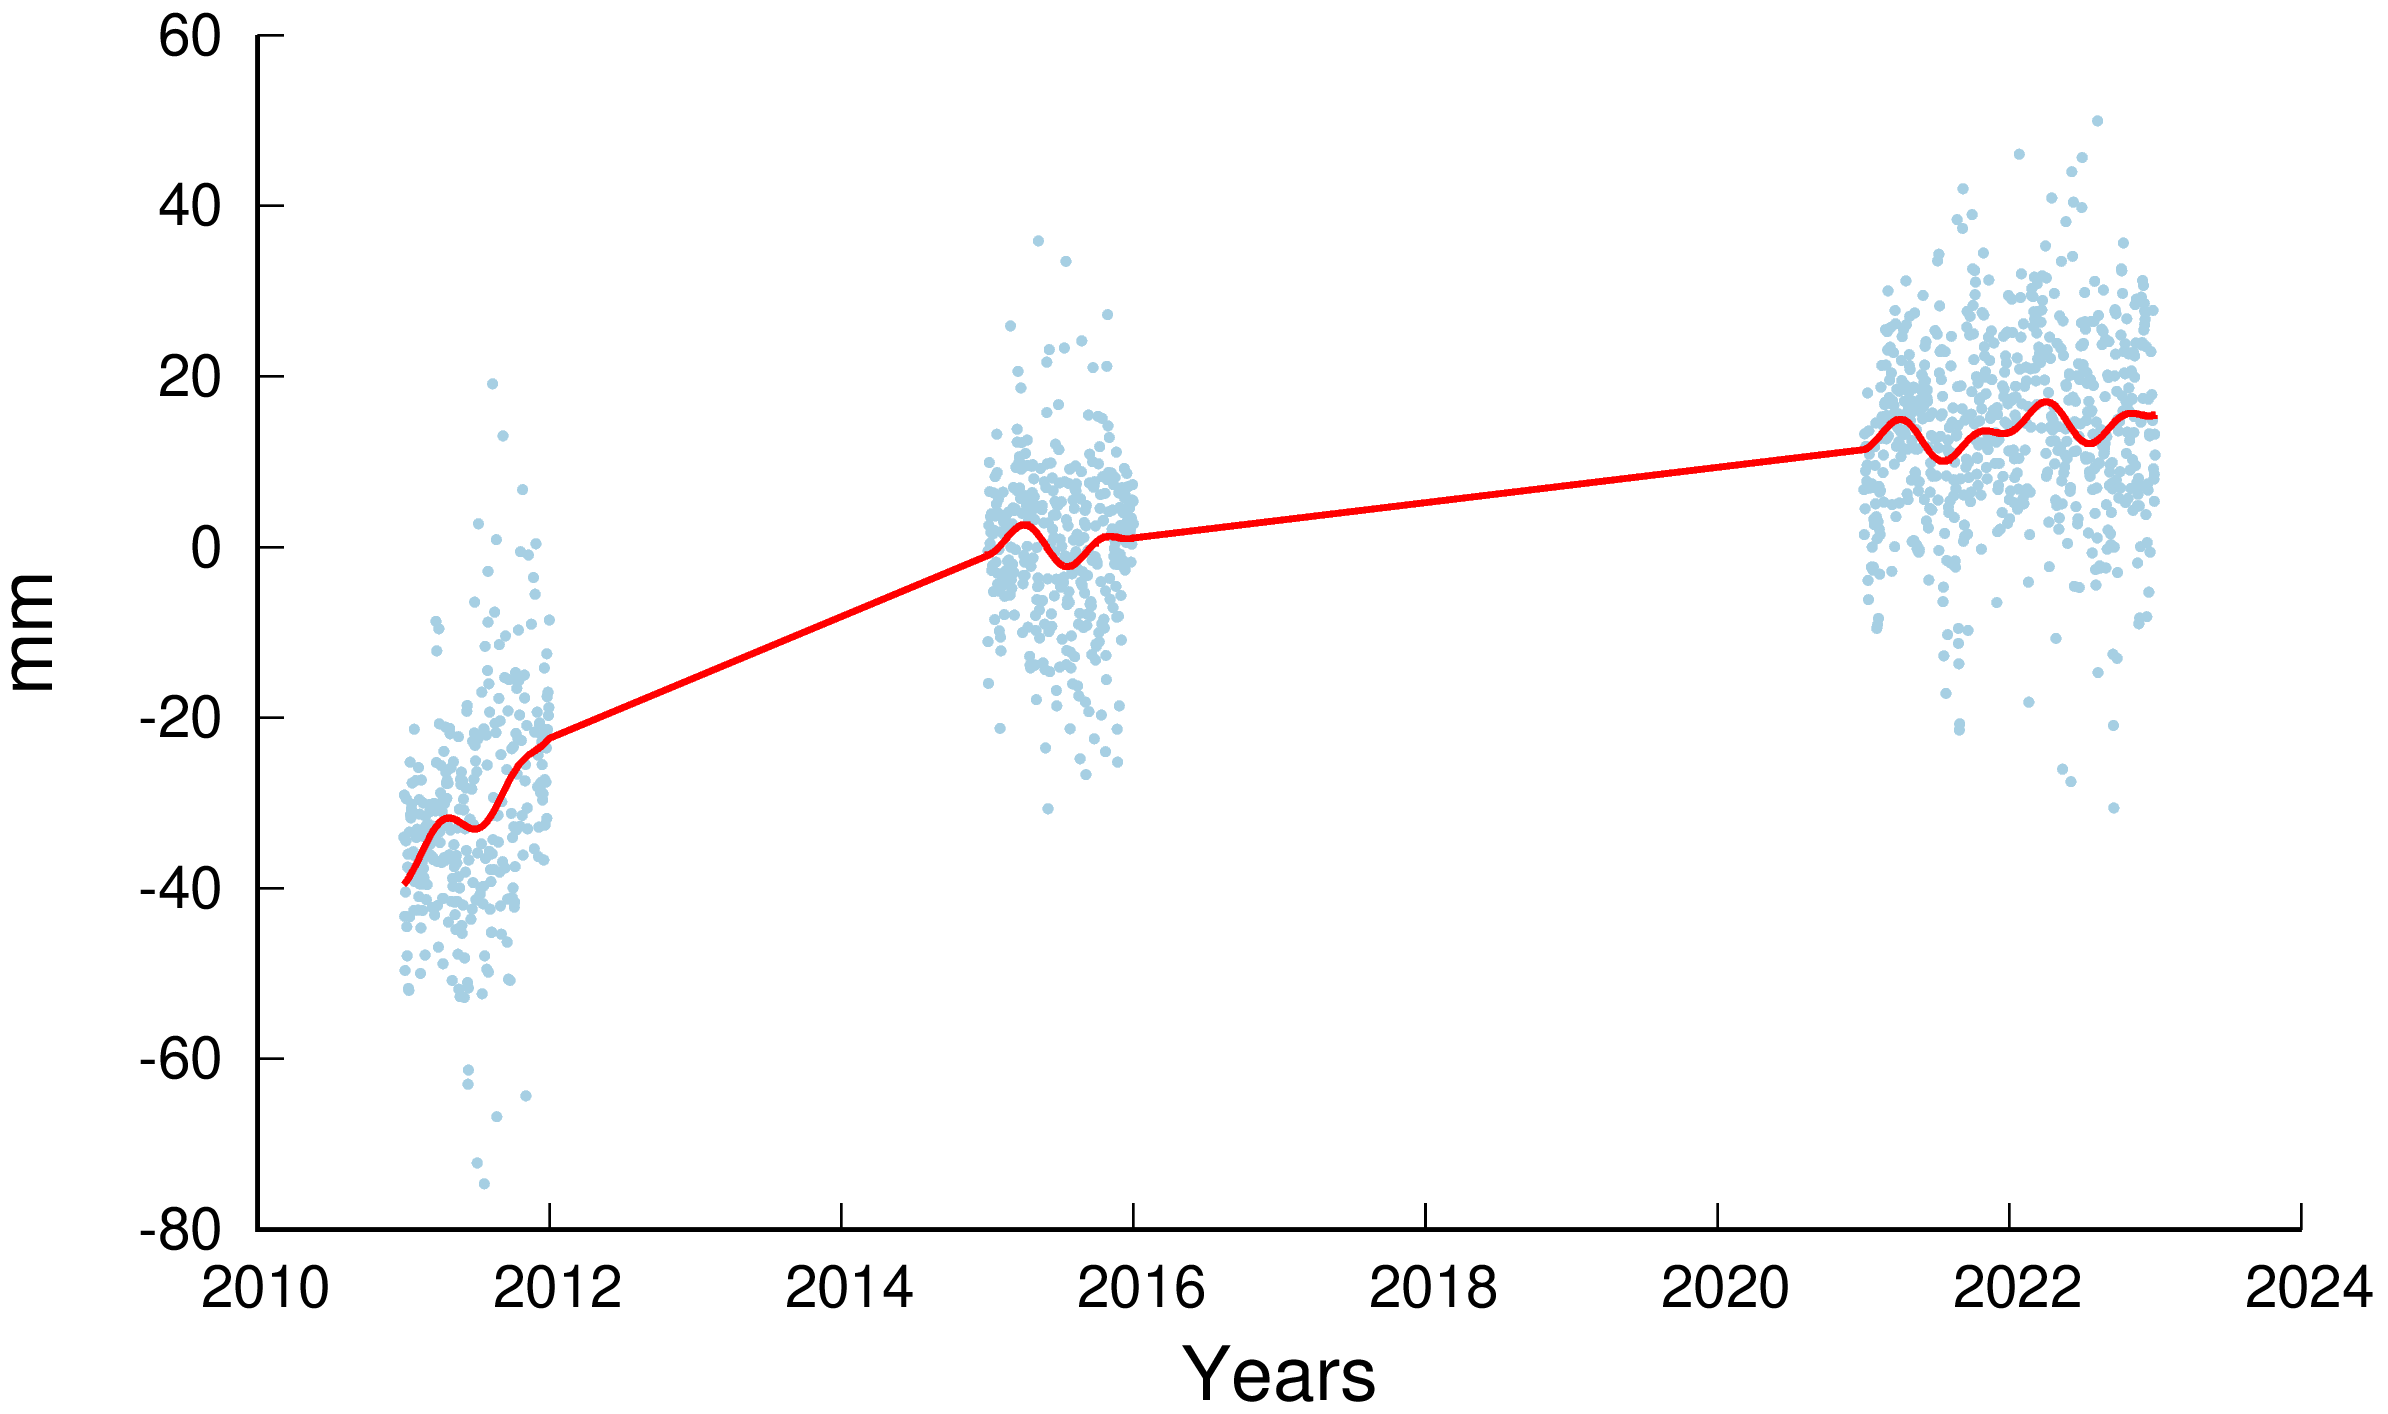
\includegraphics[width=.75\textwidth]{048a_2_data.png}
       \end{center} 
    \end{column}
    \begin{column}{.33\textwidth}
      \begin{center}
      Residuals:\textbf{048A}\\
         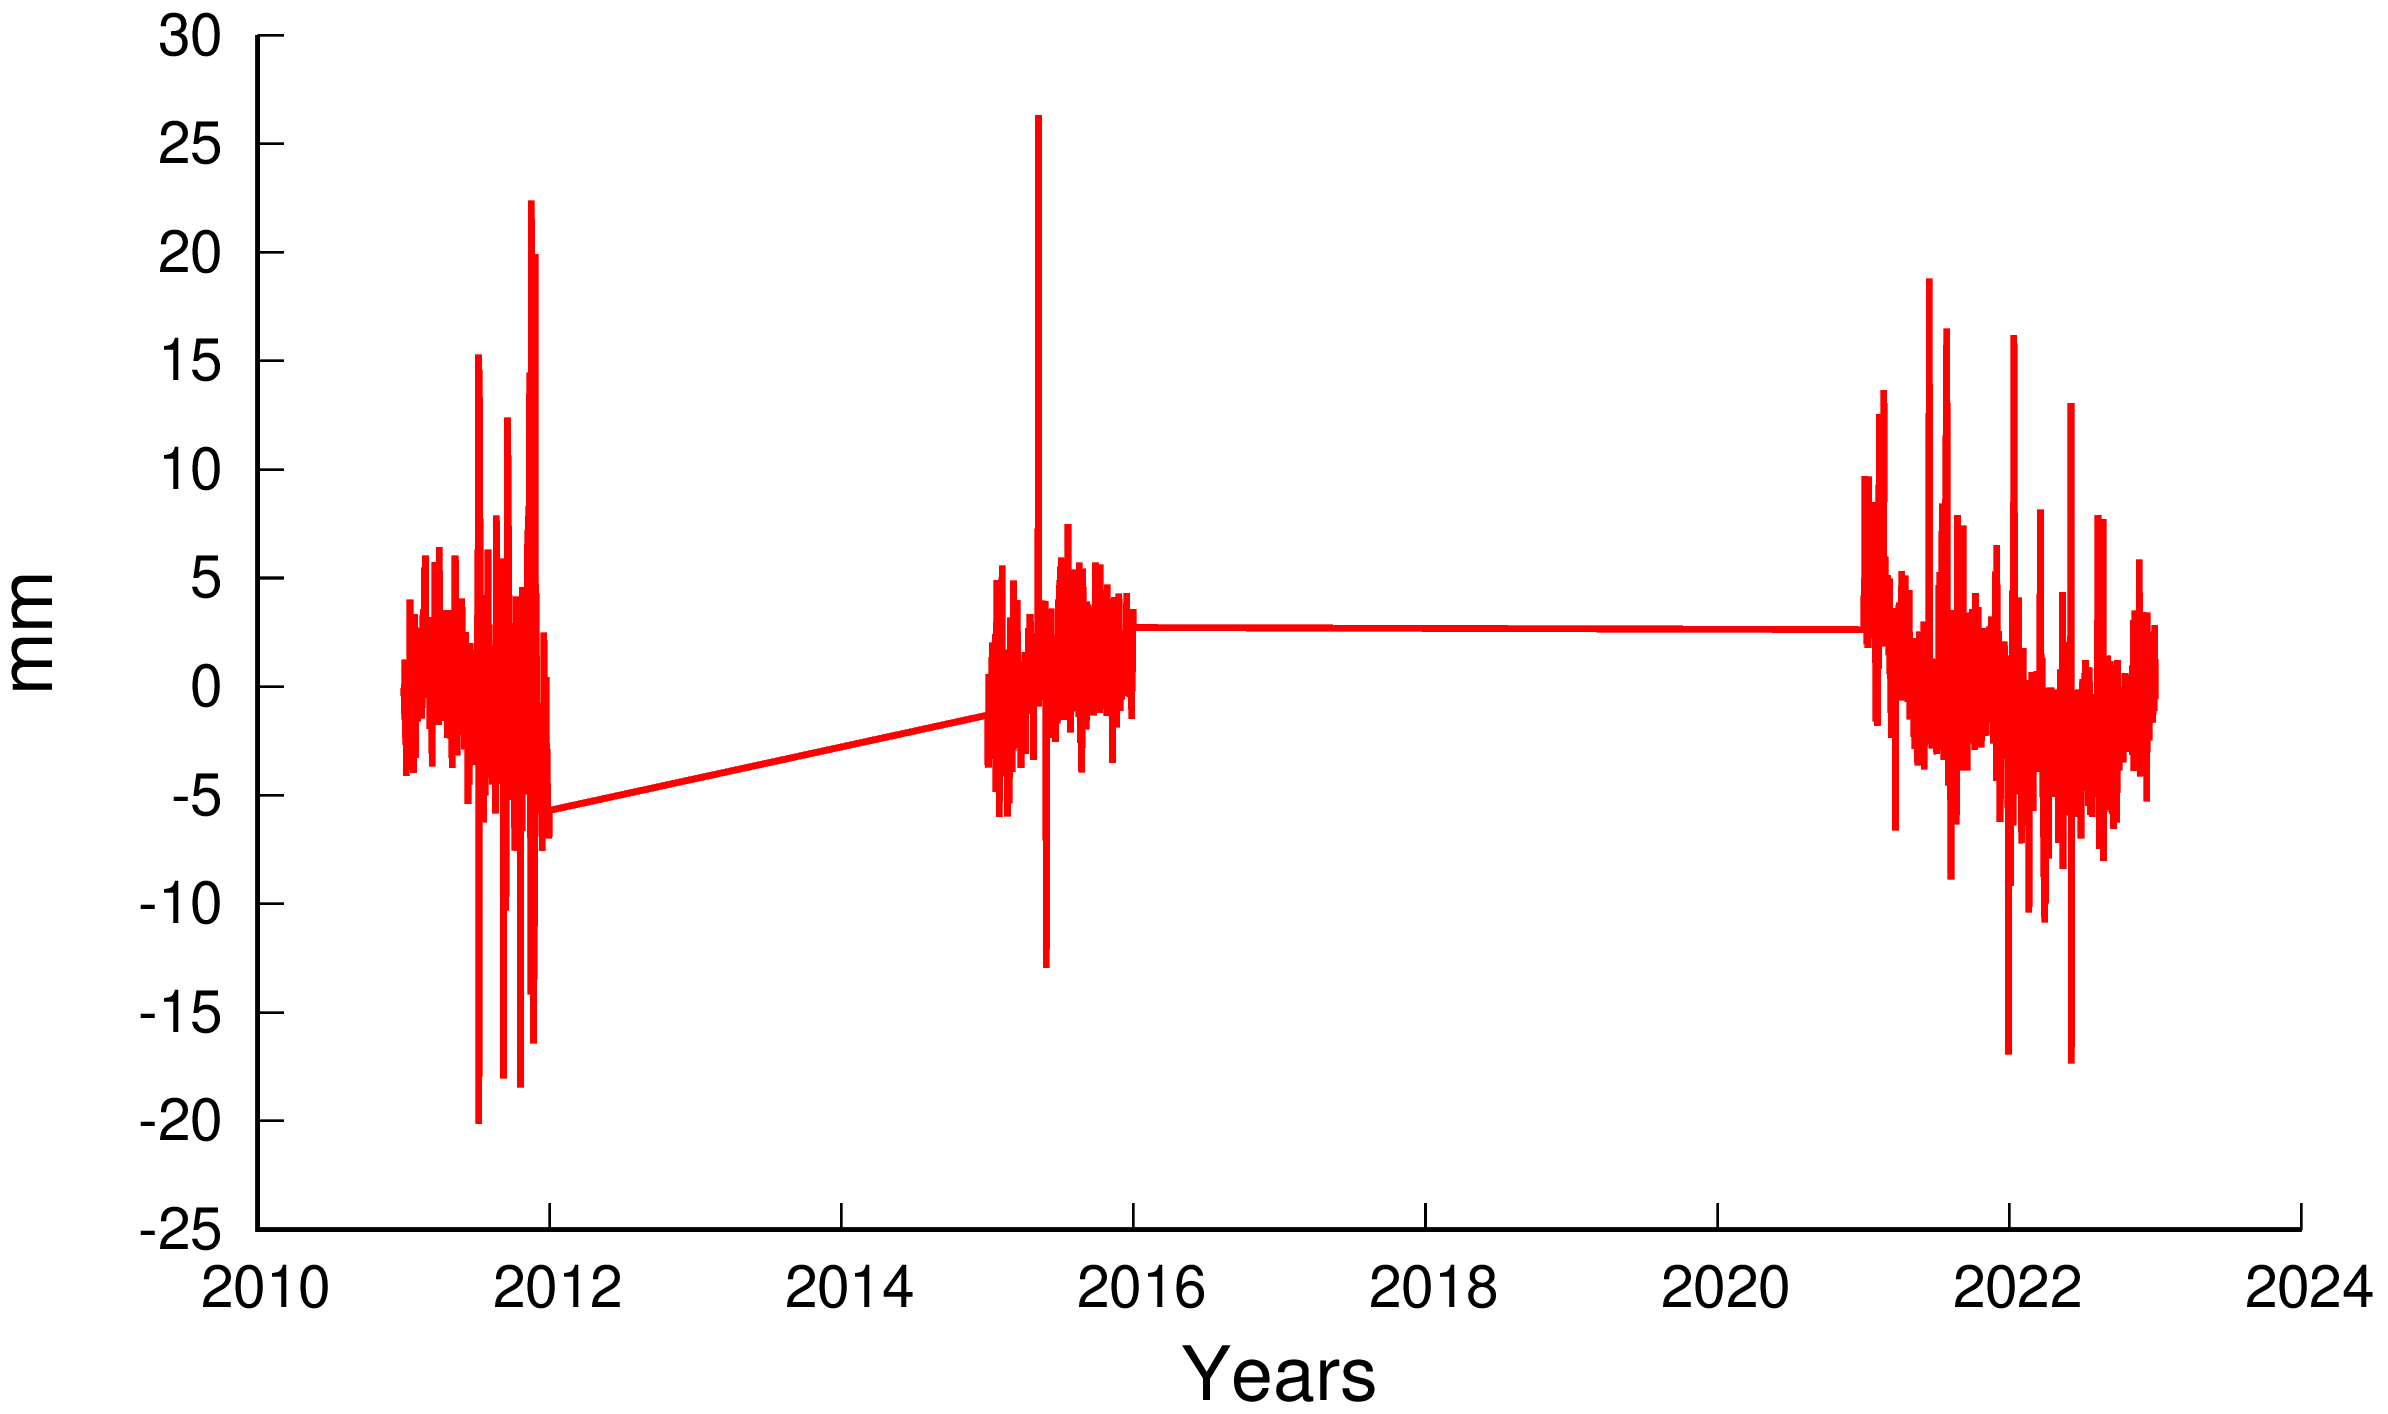
\includegraphics[width=.75\textwidth]{048a_0_res.png}\\
         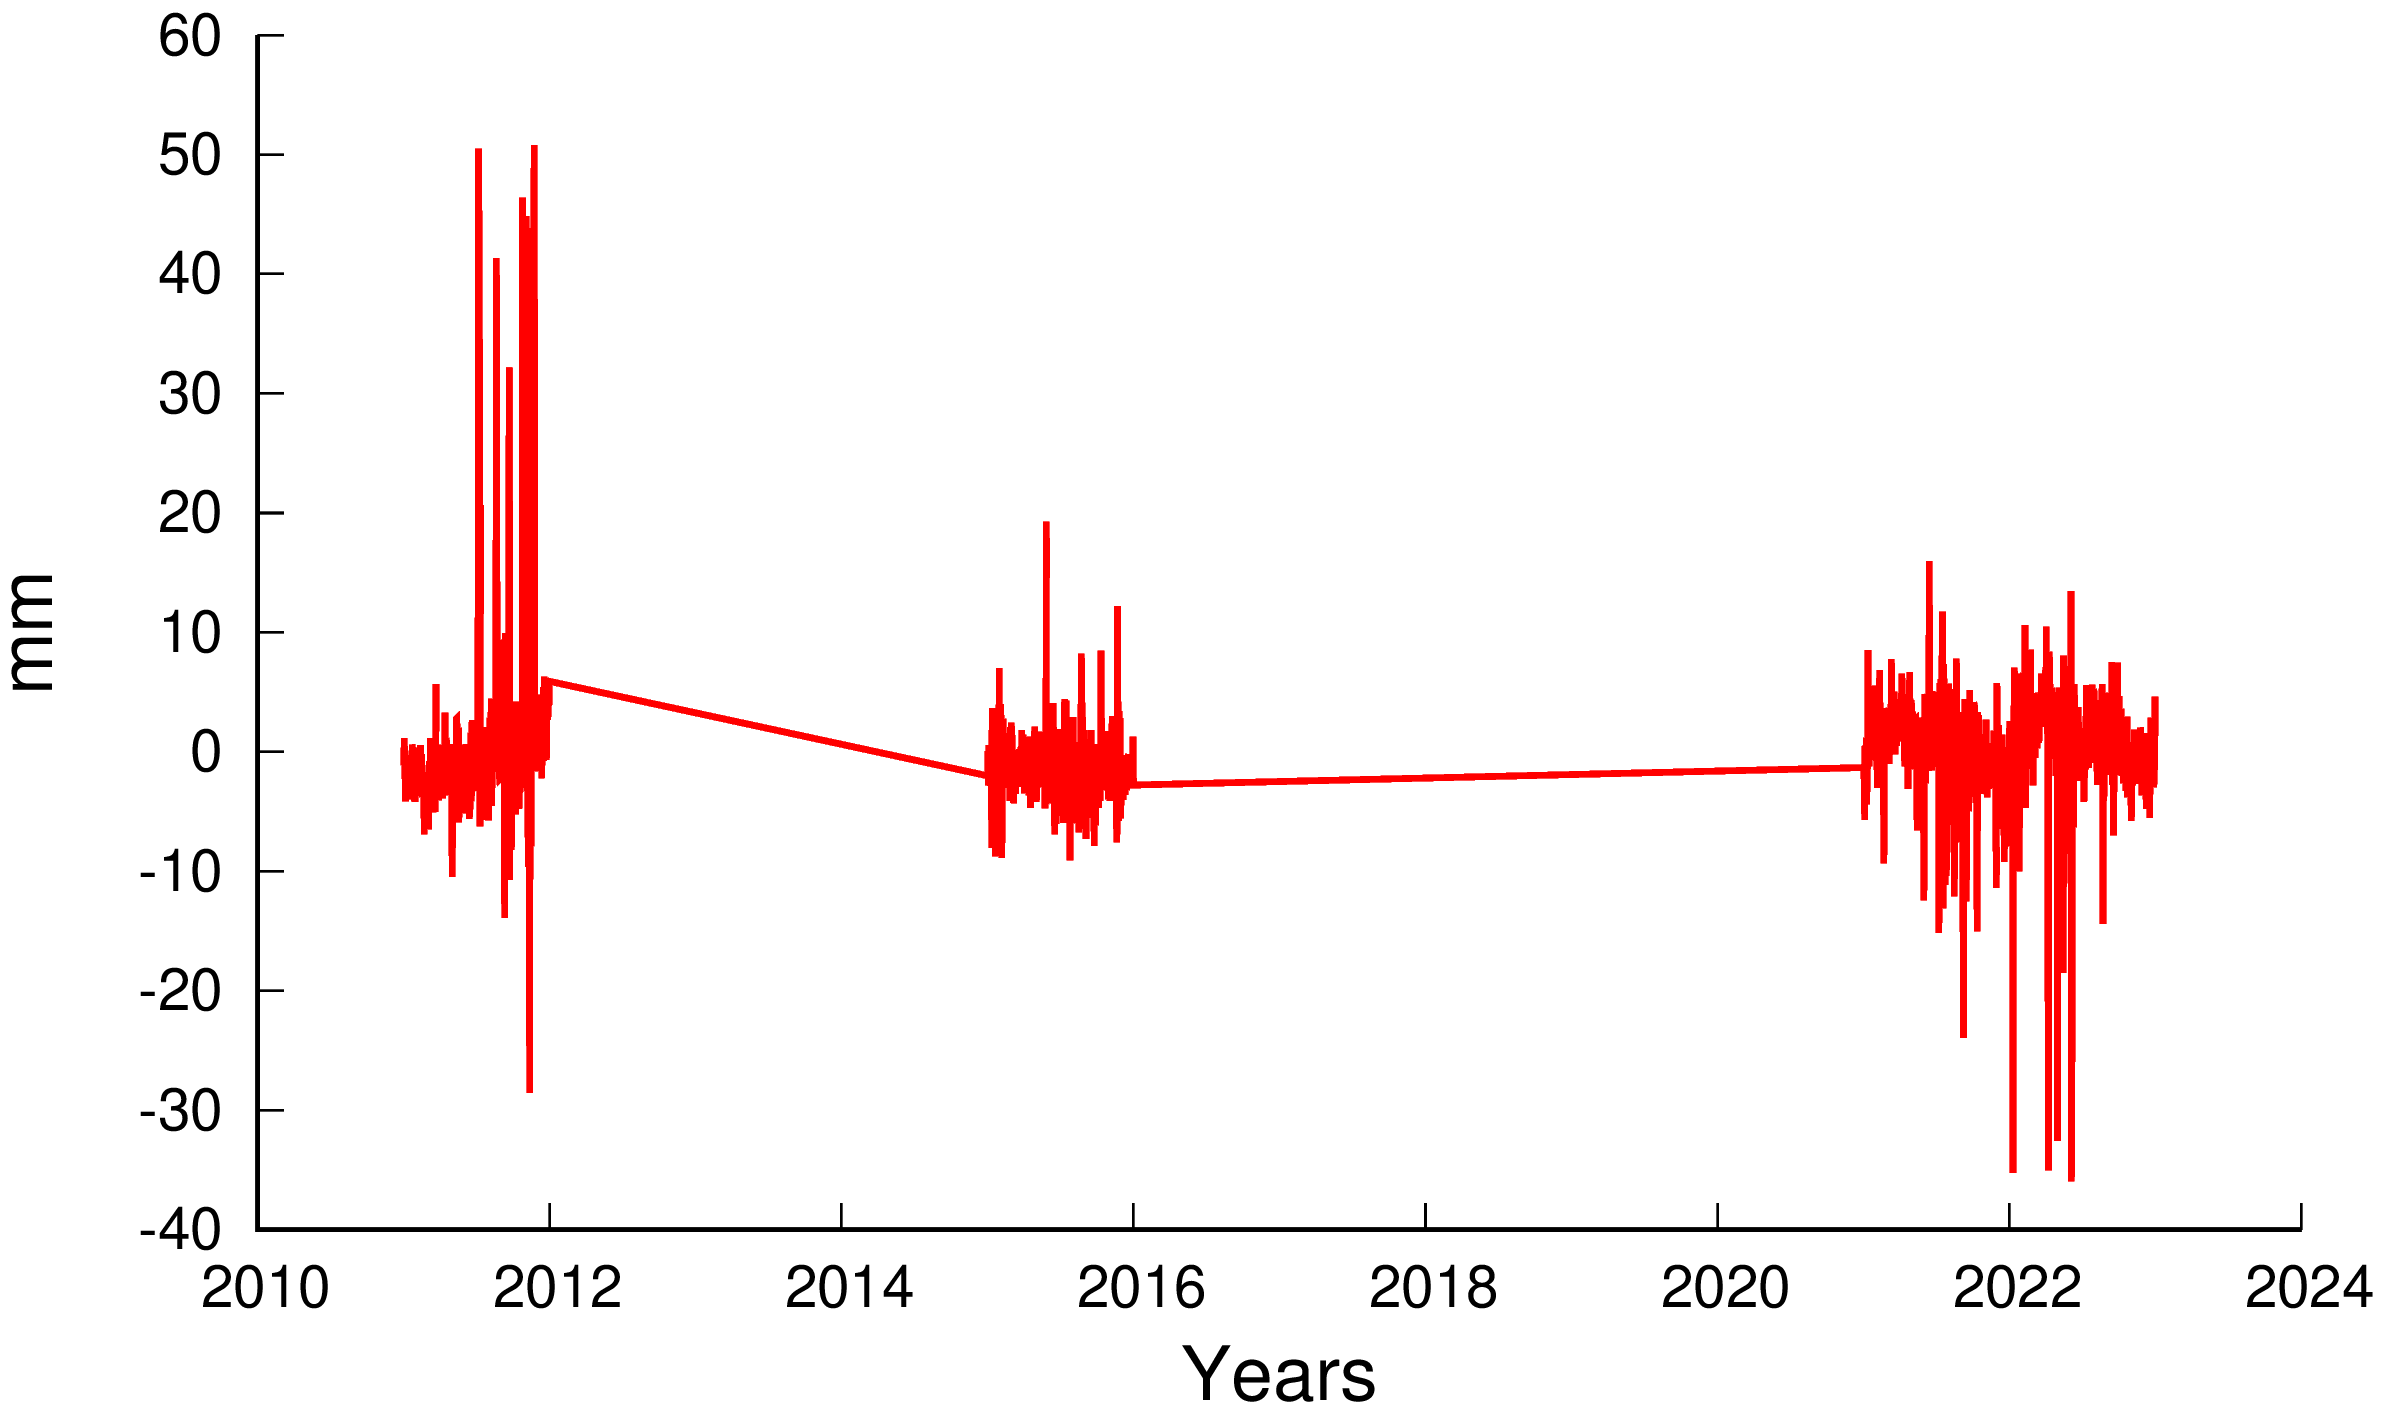
\includegraphics[width=.75\textwidth]{048a_1_res.png}\\
         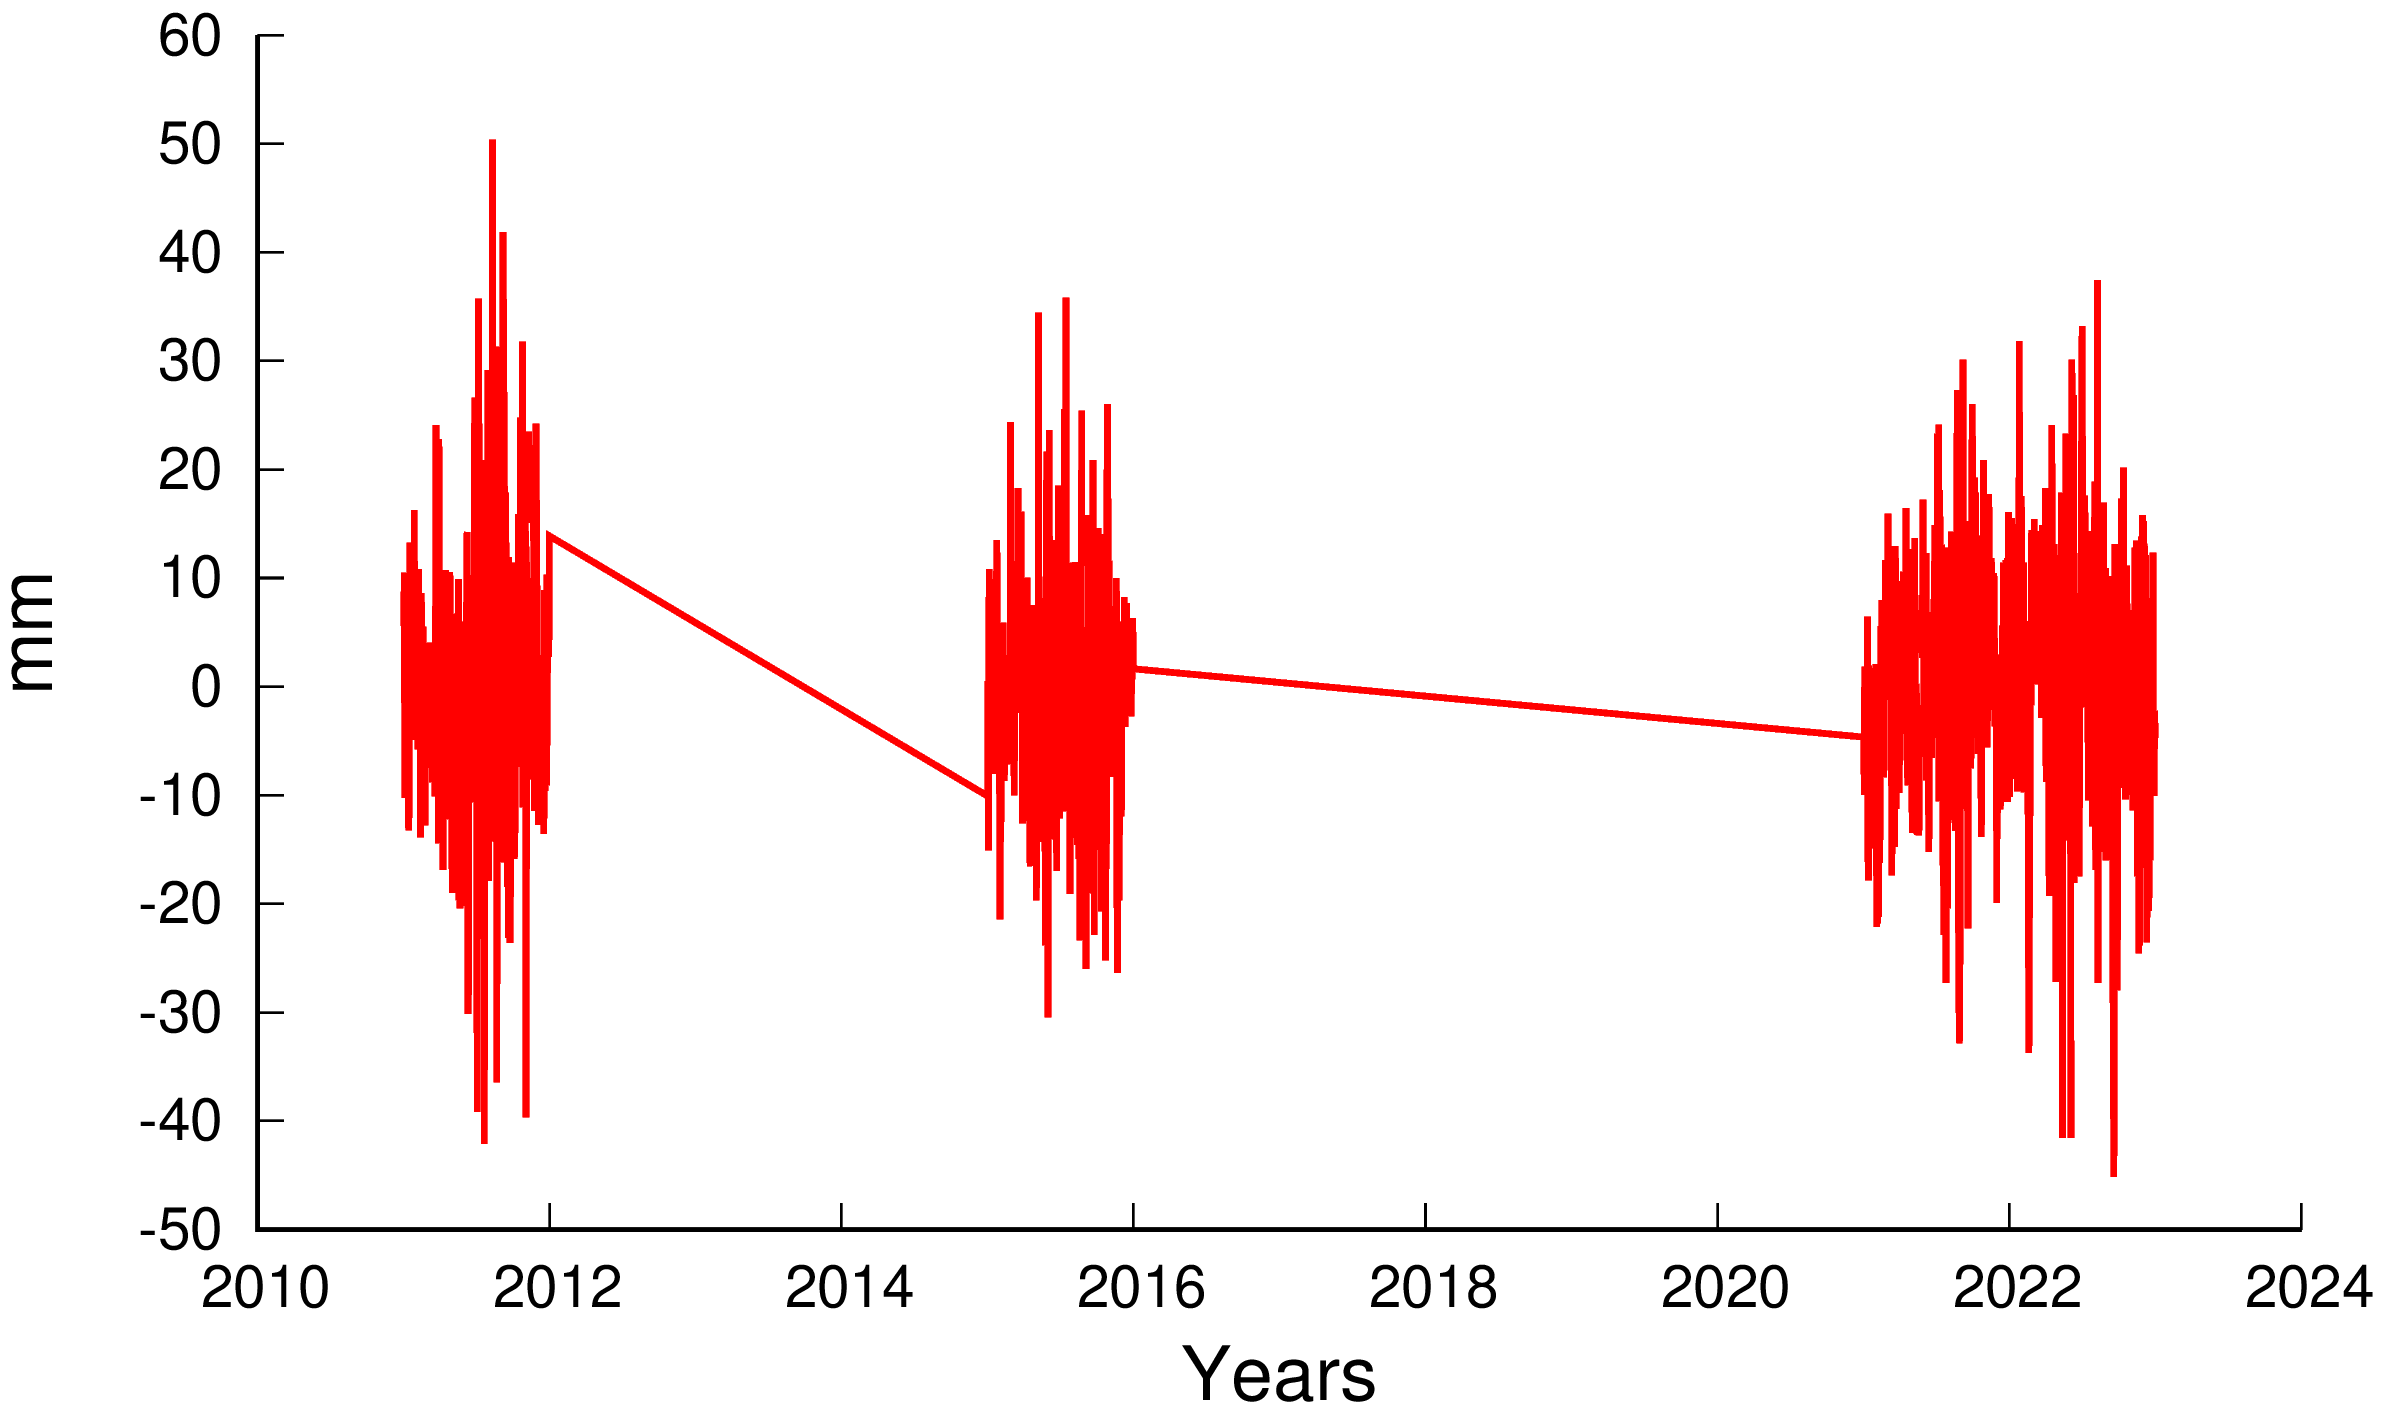
\includegraphics[width=.75\textwidth]{048a_2_res.png}
       \end{center} 
      
    \end{column}
  \end{columns}
\end{frame}
\note{}


 % ------------------------------------------------------------------------------
\begin{frame}
  \frametitle{Προσδιορισμός πεδίου ταχυτήτων - IGb14}
  \framesubtitle{}
  \label{}
  \vskip-1cm
  \begin{columns}[T]
    \begin{column}{.5\textwidth}
    Η ταχύτητες κυμαίνονται ανά συνιστώσα:
    \begin{table}[H]{\small
    \begin{center}
    \begin{tabular*}{.8\linewidth}{@{\extracolsep{\fill}} l c c}
      \toprule
        comp & min & max \\
             & \multicolumn{2}{c}{(mm/yr)}\\
      \midrule
        north & -17.9 & 15.5 \\
        east & 2.4 & 26.0\\
        up & -5.5 & 4.7 \\
      \bottomrule
    \end{tabular*}
    \end{center}}
    \end{table}
    \end{column}
    \begin{column}{.5\textwidth}
      \begin{center}
             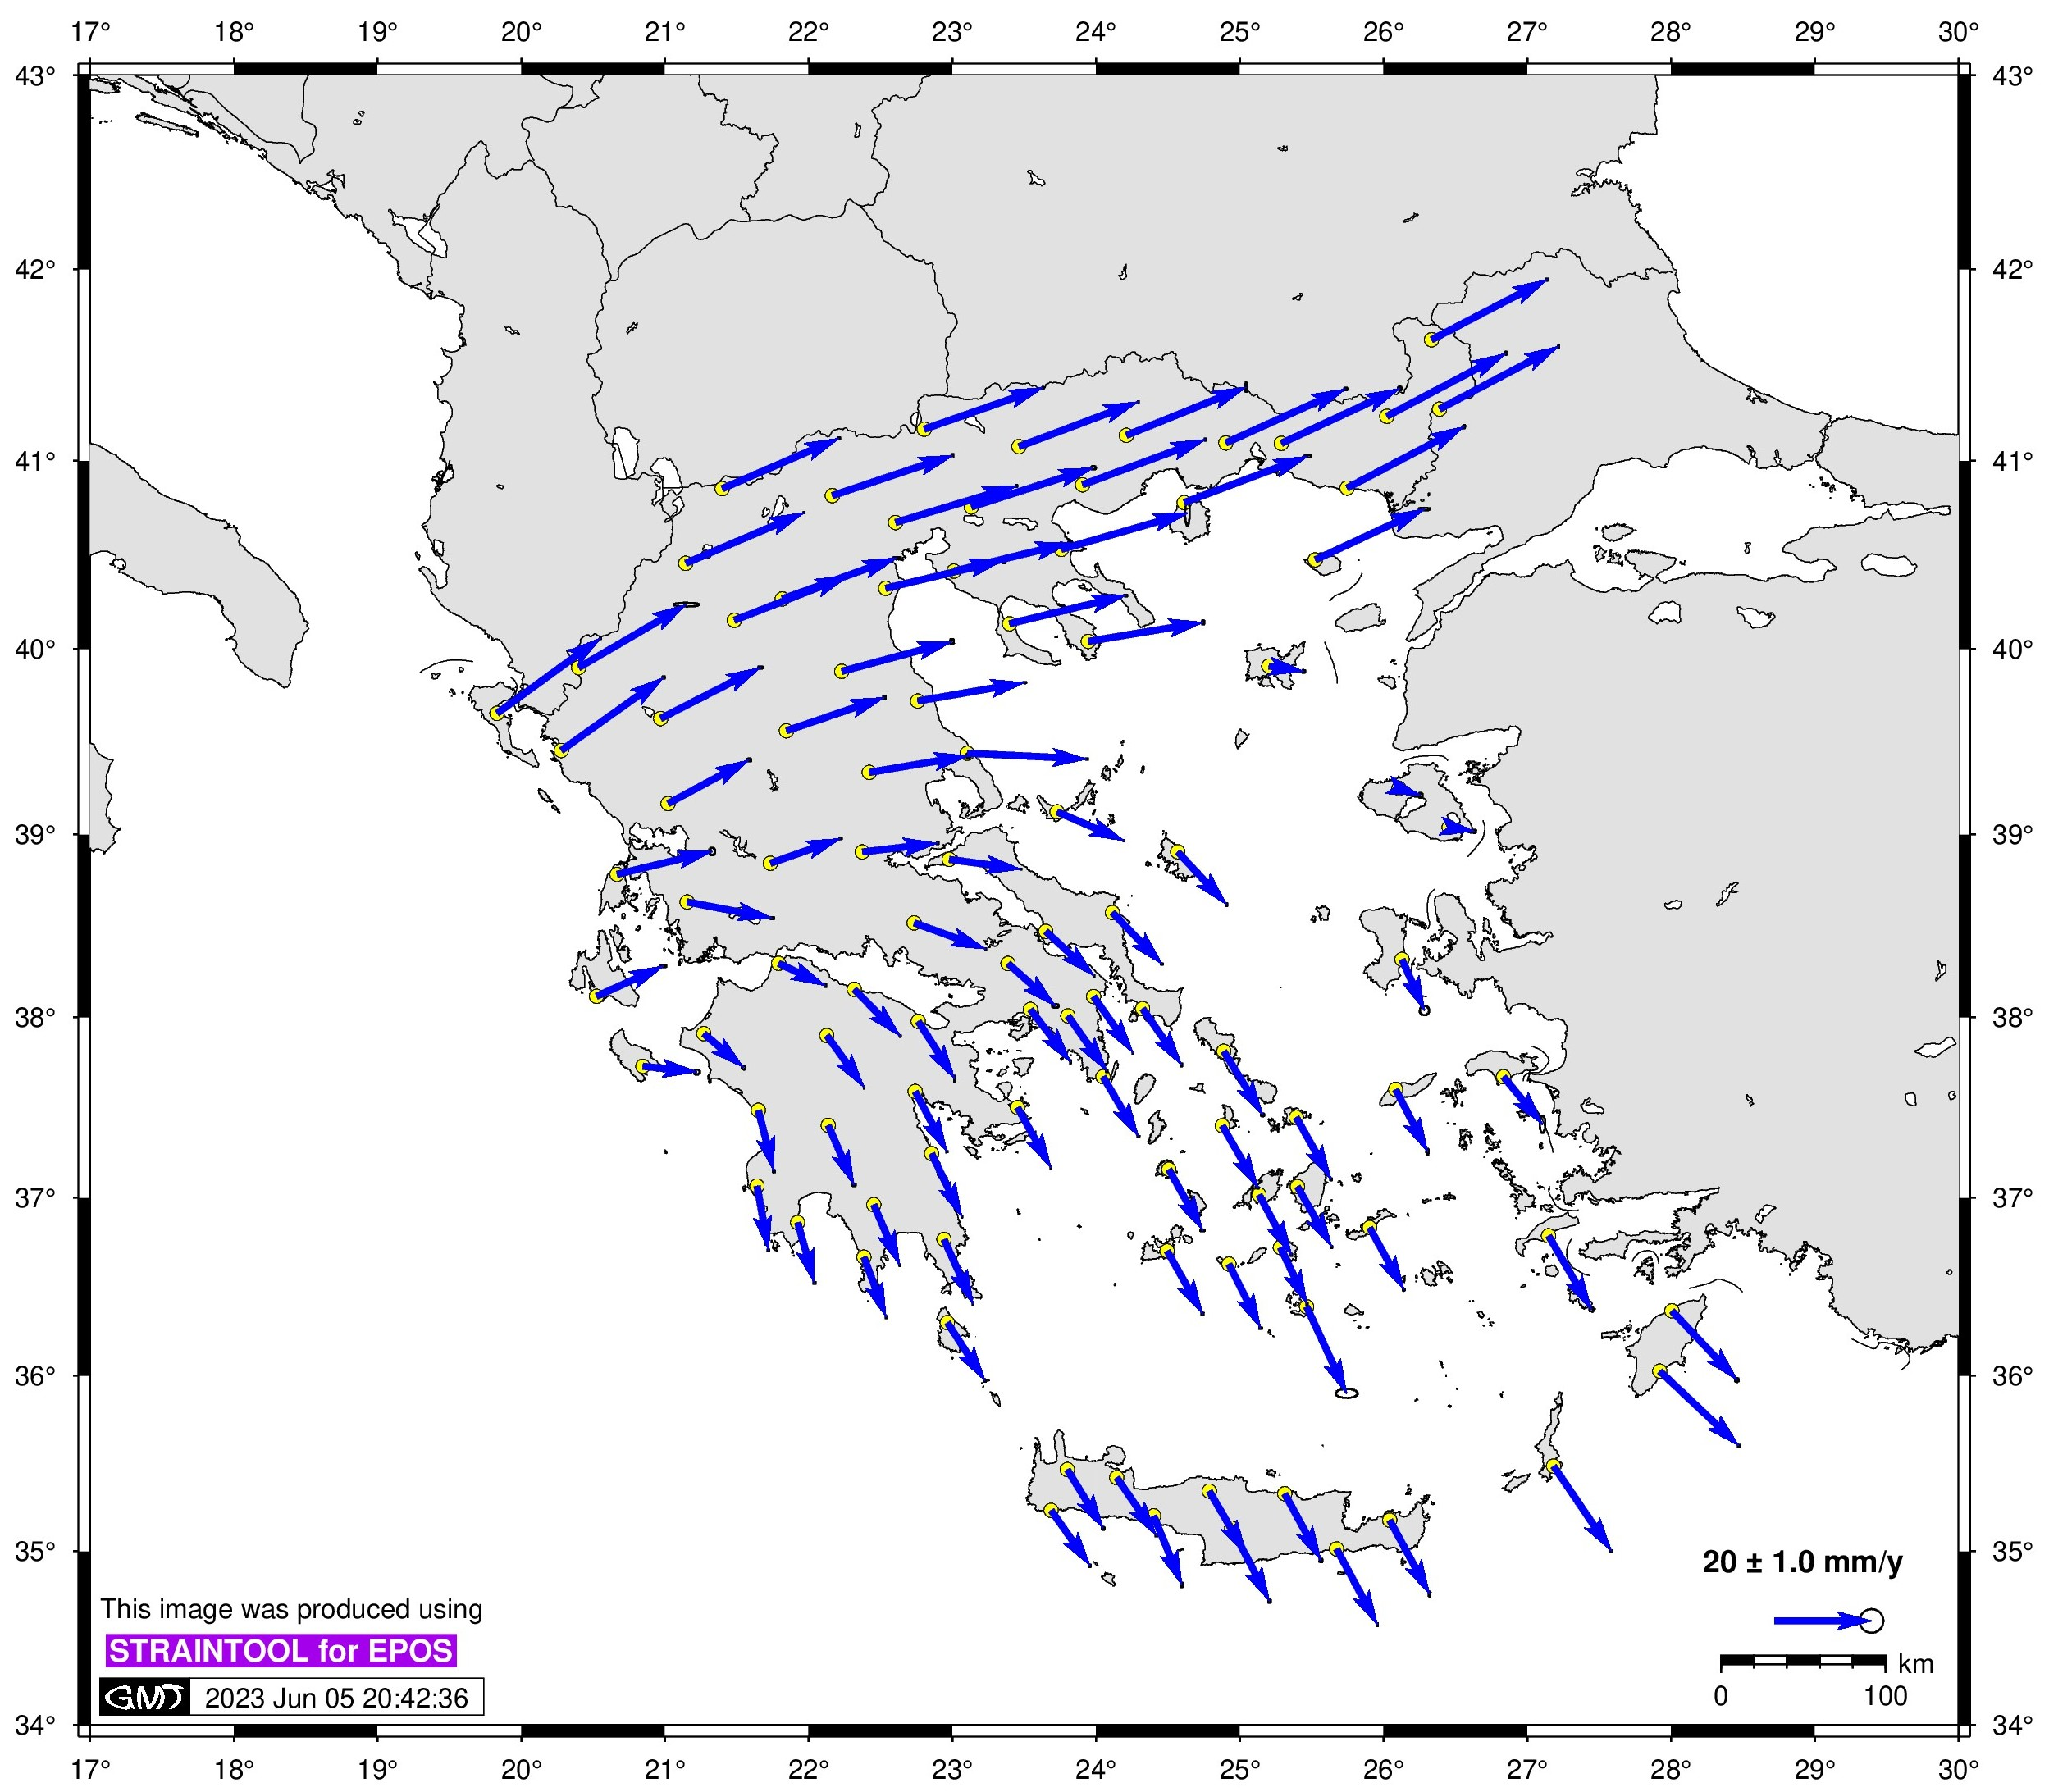
\includegraphics[width=.97\textwidth]{hepos3-output_vel.jpg}
           \end{center}     
    \end{column}
  \end{columns}
\end{frame}
\note{}

 % ------------------------------------------------------------------------------
\begin{frame}
  \frametitle{Σύγκριση πεδίου ταχυτήτων}
  \framesubtitle{}
  \label{}
  \vskip-1cm
  \begin{columns}[T]
    \begin{column}{.5\textwidth}
    \begin{center}
      \texttt{DSO\_GRC\_2021}\\
      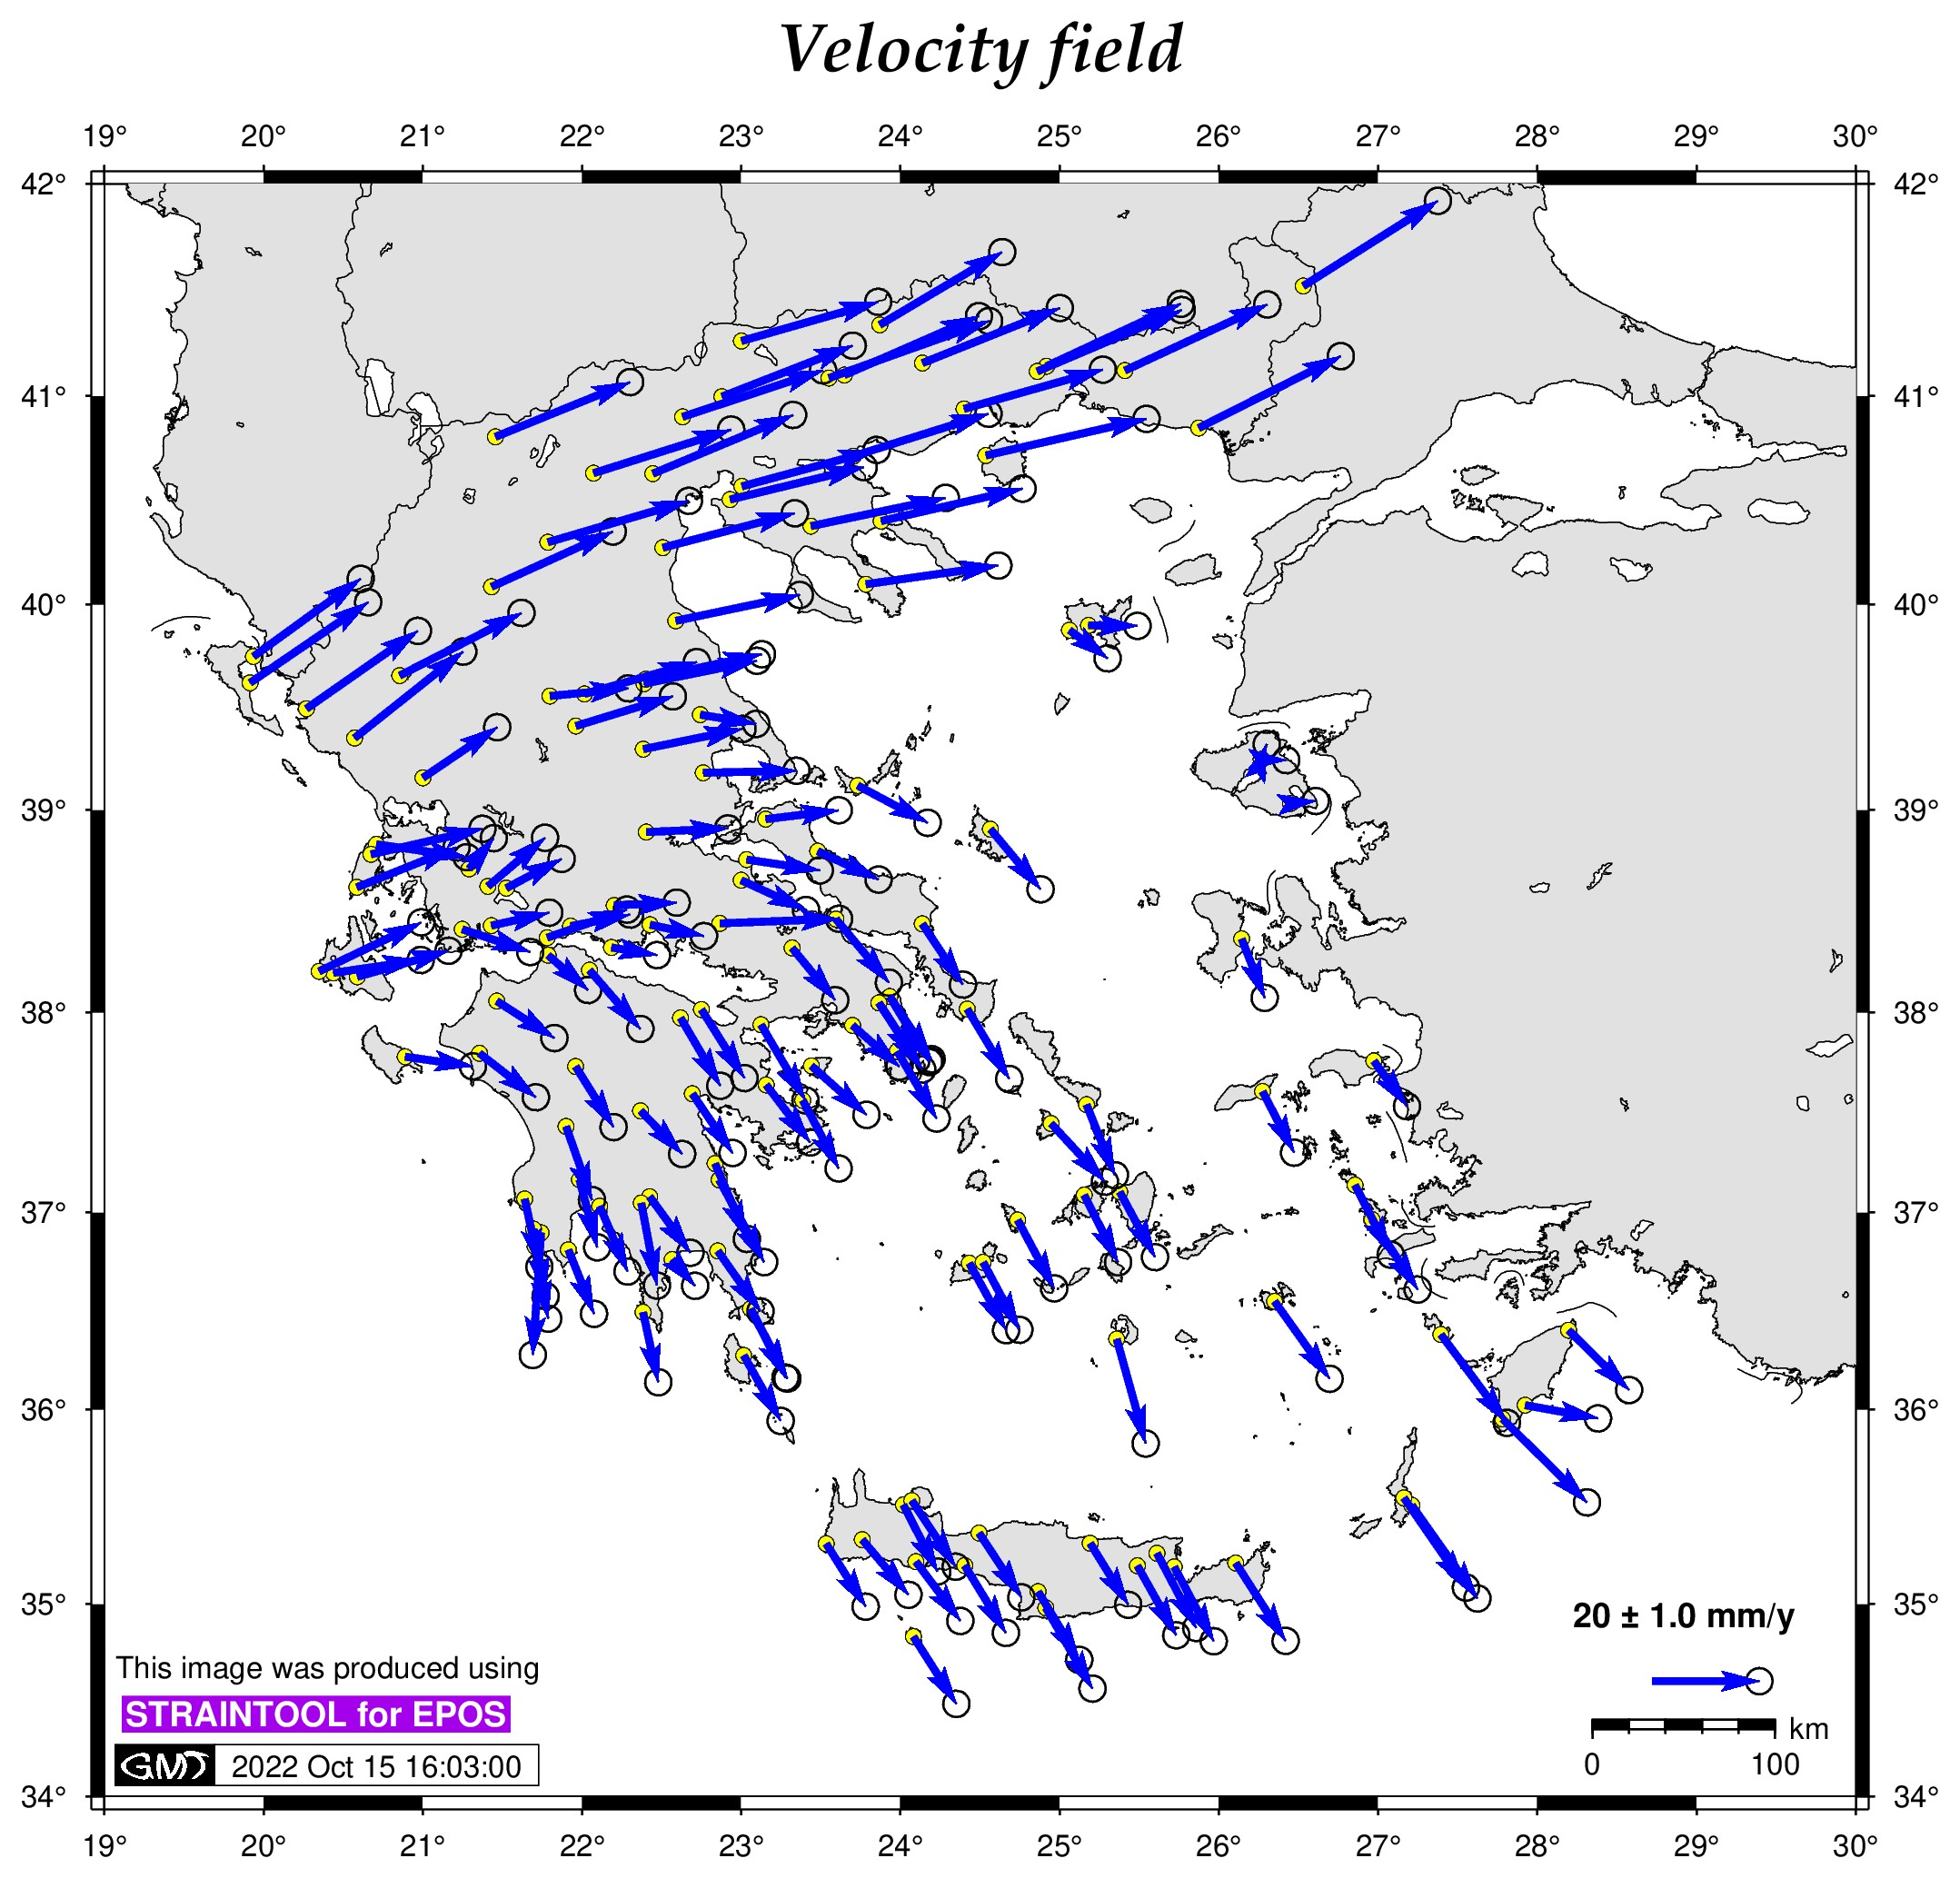
\includegraphics[width=.97\textwidth]{gr-output_vel.jpg}
    \end{center}
    \end{column}
    \begin{column}{.5\textwidth}
      \begin{center}
        \texttt{DSO\_HPS\_2022}\\
        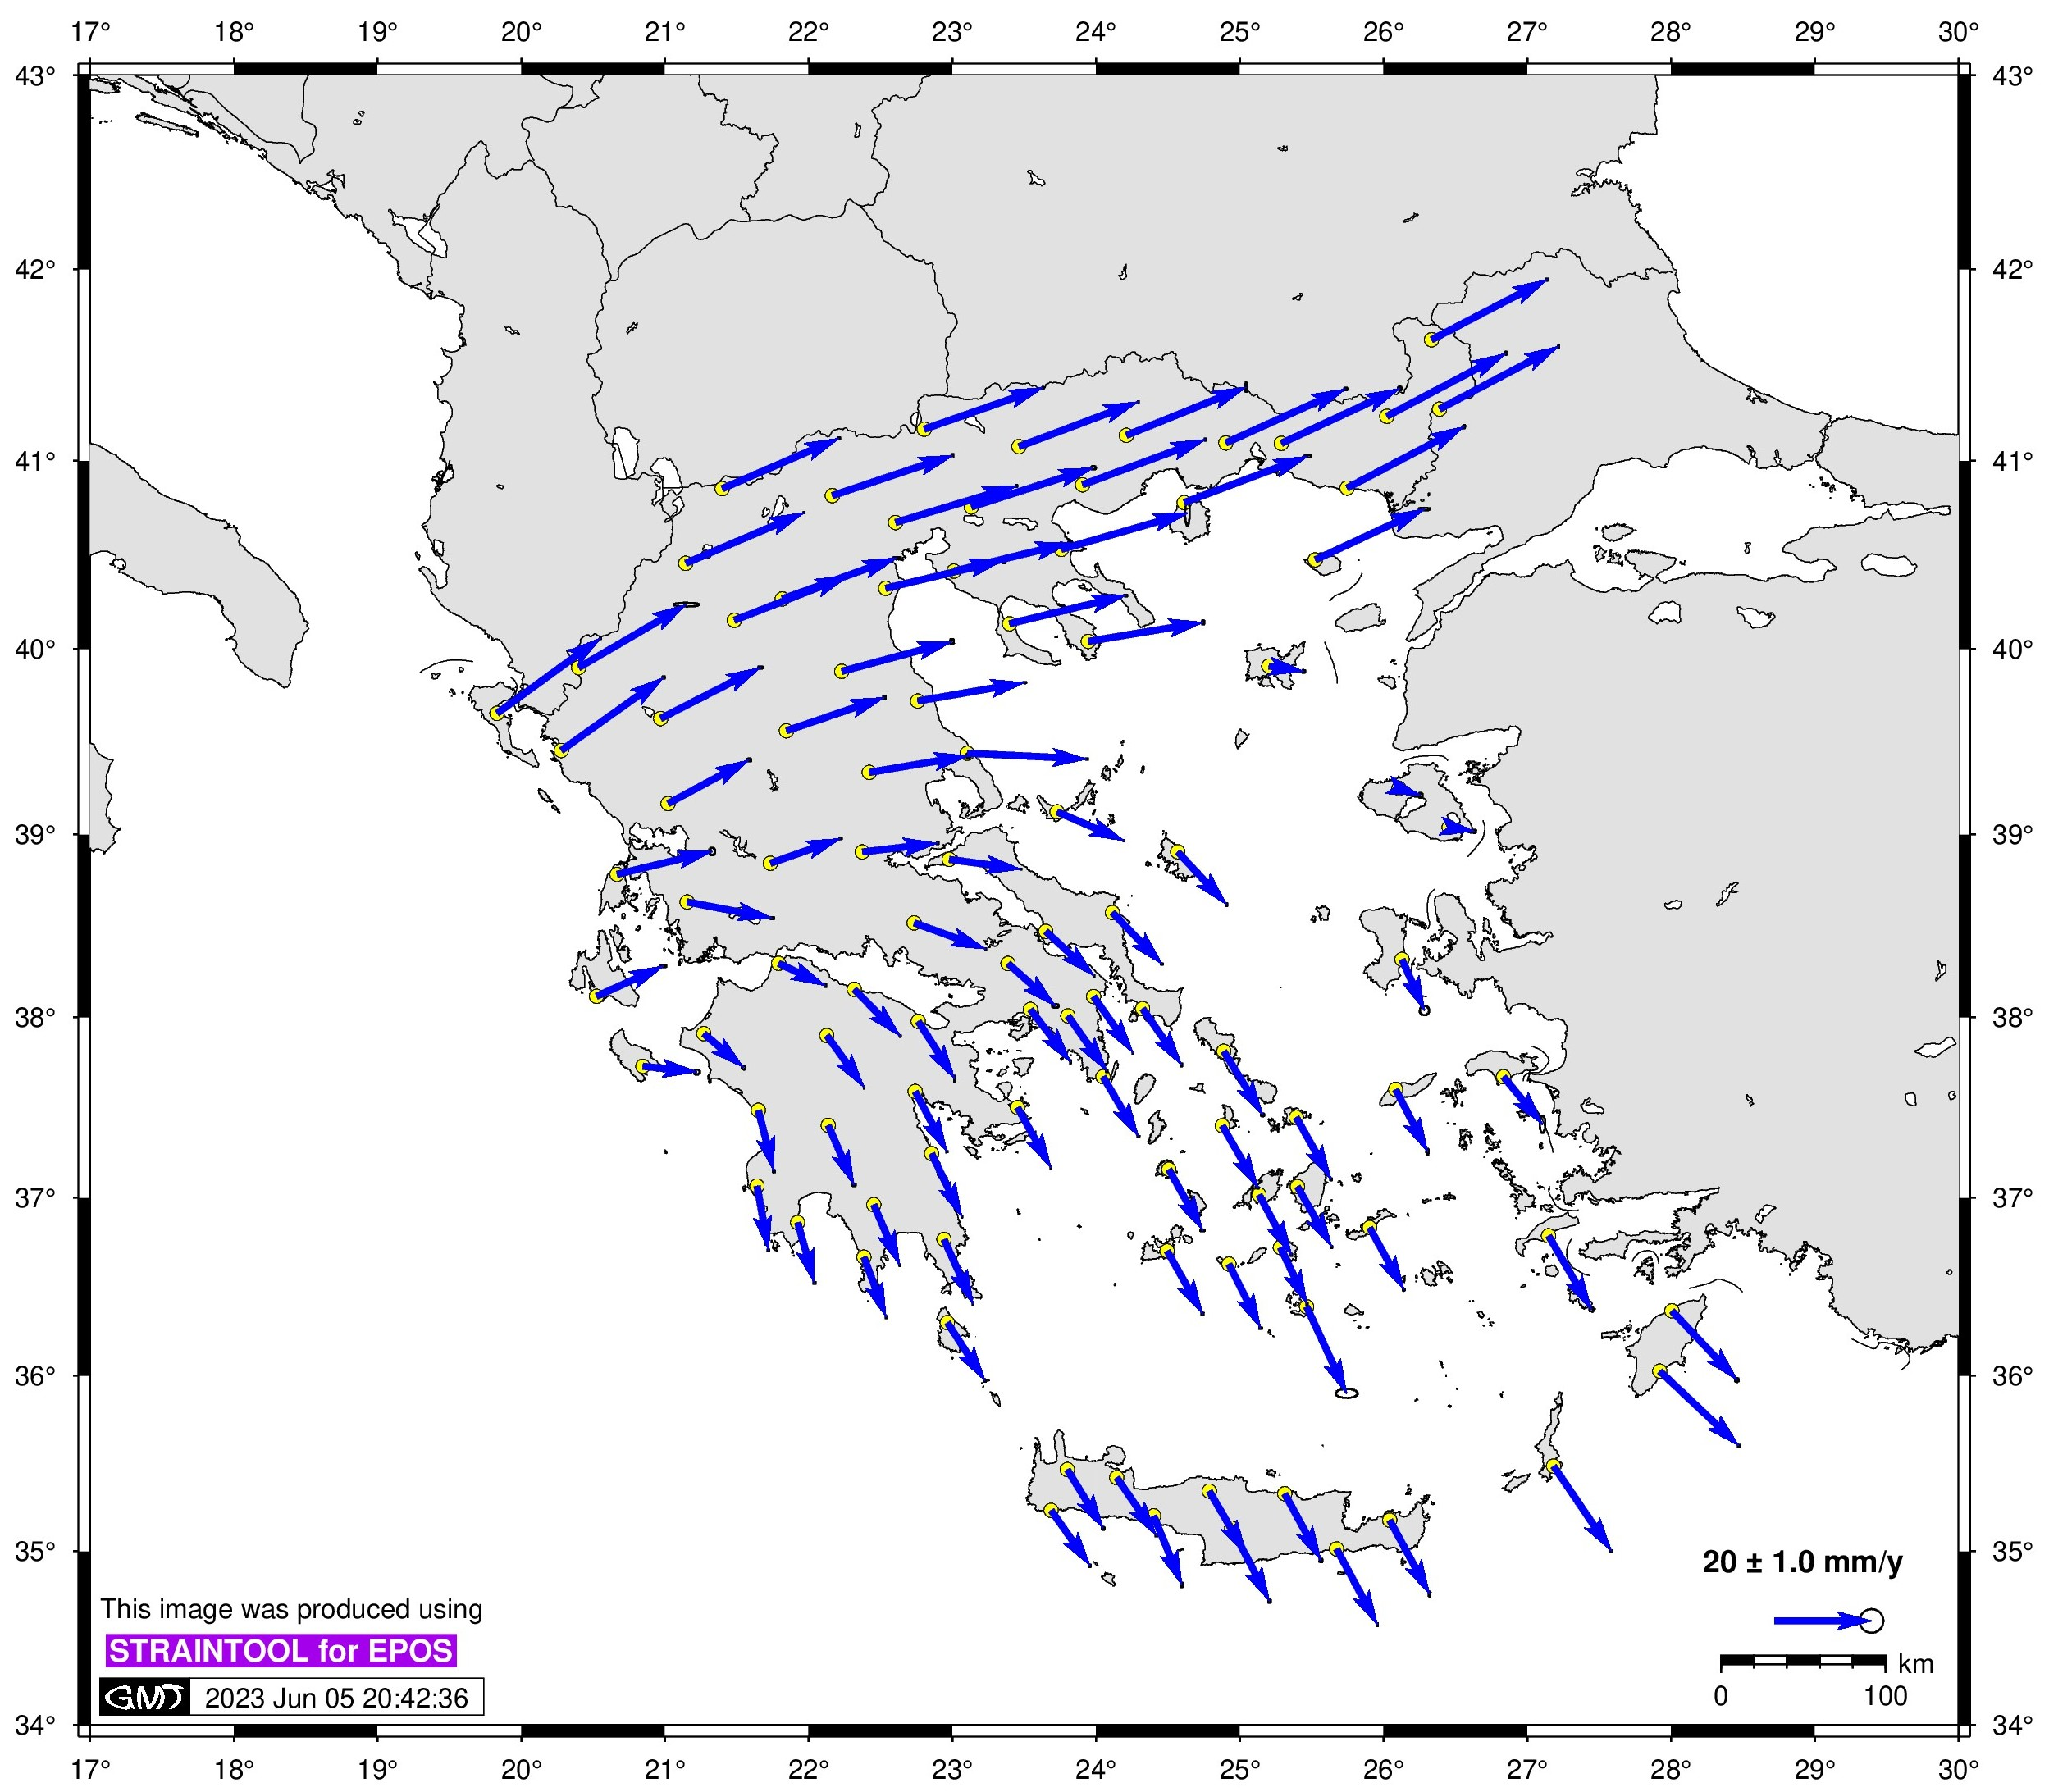
\includegraphics[width=.97\textwidth]{hepos3-output_vel.jpg}
      \end{center}    
    \end{column}
  \end{columns}
\end{frame}
\note{}

 % ------------------------------------------------------------------------------
\begin{frame}
  \frametitle{Αντί επιλόγου ...}
  \framesubtitle{}
  \label{}
  \begin{itemize}\setlength\itemsep{1em}
    \item
    \item
  \end{itemize}
\end{frame}
\note{}